% Options for packages loaded elsewhere
\PassOptionsToPackage{unicode}{hyperref}
\PassOptionsToPackage{hyphens}{url}
\PassOptionsToPackage{dvipsnames,svgnames,x11names}{xcolor}
%
\documentclass[
  letterpaper,
  DIV=11,
  numbers=noendperiod]{scrartcl}

\usepackage{amsmath,amssymb}
\usepackage{iftex}
\ifPDFTeX
  \usepackage[T1]{fontenc}
  \usepackage[utf8]{inputenc}
  \usepackage{textcomp} % provide euro and other symbols
\else % if luatex or xetex
  \usepackage{unicode-math}
  \defaultfontfeatures{Scale=MatchLowercase}
  \defaultfontfeatures[\rmfamily]{Ligatures=TeX,Scale=1}
\fi
\usepackage{lmodern}
\ifPDFTeX\else  
    % xetex/luatex font selection
\fi
% Use upquote if available, for straight quotes in verbatim environments
\IfFileExists{upquote.sty}{\usepackage{upquote}}{}
\IfFileExists{microtype.sty}{% use microtype if available
  \usepackage[]{microtype}
  \UseMicrotypeSet[protrusion]{basicmath} % disable protrusion for tt fonts
}{}
\makeatletter
\@ifundefined{KOMAClassName}{% if non-KOMA class
  \IfFileExists{parskip.sty}{%
    \usepackage{parskip}
  }{% else
    \setlength{\parindent}{0pt}
    \setlength{\parskip}{6pt plus 2pt minus 1pt}}
}{% if KOMA class
  \KOMAoptions{parskip=half}}
\makeatother
\usepackage{xcolor}
\setlength{\emergencystretch}{3em} % prevent overfull lines
\setcounter{secnumdepth}{5}
% Make \paragraph and \subparagraph free-standing
\ifx\paragraph\undefined\else
  \let\oldparagraph\paragraph
  \renewcommand{\paragraph}[1]{\oldparagraph{#1}\mbox{}}
\fi
\ifx\subparagraph\undefined\else
  \let\oldsubparagraph\subparagraph
  \renewcommand{\subparagraph}[1]{\oldsubparagraph{#1}\mbox{}}
\fi

\usepackage{color}
\usepackage{fancyvrb}
\newcommand{\VerbBar}{|}
\newcommand{\VERB}{\Verb[commandchars=\\\{\}]}
\DefineVerbatimEnvironment{Highlighting}{Verbatim}{commandchars=\\\{\}}
% Add ',fontsize=\small' for more characters per line
\usepackage{framed}
\definecolor{shadecolor}{RGB}{241,243,245}
\newenvironment{Shaded}{\begin{snugshade}}{\end{snugshade}}
\newcommand{\AlertTok}[1]{\textcolor[rgb]{0.68,0.00,0.00}{#1}}
\newcommand{\AnnotationTok}[1]{\textcolor[rgb]{0.37,0.37,0.37}{#1}}
\newcommand{\AttributeTok}[1]{\textcolor[rgb]{0.40,0.45,0.13}{#1}}
\newcommand{\BaseNTok}[1]{\textcolor[rgb]{0.68,0.00,0.00}{#1}}
\newcommand{\BuiltInTok}[1]{\textcolor[rgb]{0.00,0.23,0.31}{#1}}
\newcommand{\CharTok}[1]{\textcolor[rgb]{0.13,0.47,0.30}{#1}}
\newcommand{\CommentTok}[1]{\textcolor[rgb]{0.37,0.37,0.37}{#1}}
\newcommand{\CommentVarTok}[1]{\textcolor[rgb]{0.37,0.37,0.37}{\textit{#1}}}
\newcommand{\ConstantTok}[1]{\textcolor[rgb]{0.56,0.35,0.01}{#1}}
\newcommand{\ControlFlowTok}[1]{\textcolor[rgb]{0.00,0.23,0.31}{#1}}
\newcommand{\DataTypeTok}[1]{\textcolor[rgb]{0.68,0.00,0.00}{#1}}
\newcommand{\DecValTok}[1]{\textcolor[rgb]{0.68,0.00,0.00}{#1}}
\newcommand{\DocumentationTok}[1]{\textcolor[rgb]{0.37,0.37,0.37}{\textit{#1}}}
\newcommand{\ErrorTok}[1]{\textcolor[rgb]{0.68,0.00,0.00}{#1}}
\newcommand{\ExtensionTok}[1]{\textcolor[rgb]{0.00,0.23,0.31}{#1}}
\newcommand{\FloatTok}[1]{\textcolor[rgb]{0.68,0.00,0.00}{#1}}
\newcommand{\FunctionTok}[1]{\textcolor[rgb]{0.28,0.35,0.67}{#1}}
\newcommand{\ImportTok}[1]{\textcolor[rgb]{0.00,0.46,0.62}{#1}}
\newcommand{\InformationTok}[1]{\textcolor[rgb]{0.37,0.37,0.37}{#1}}
\newcommand{\KeywordTok}[1]{\textcolor[rgb]{0.00,0.23,0.31}{#1}}
\newcommand{\NormalTok}[1]{\textcolor[rgb]{0.00,0.23,0.31}{#1}}
\newcommand{\OperatorTok}[1]{\textcolor[rgb]{0.37,0.37,0.37}{#1}}
\newcommand{\OtherTok}[1]{\textcolor[rgb]{0.00,0.23,0.31}{#1}}
\newcommand{\PreprocessorTok}[1]{\textcolor[rgb]{0.68,0.00,0.00}{#1}}
\newcommand{\RegionMarkerTok}[1]{\textcolor[rgb]{0.00,0.23,0.31}{#1}}
\newcommand{\SpecialCharTok}[1]{\textcolor[rgb]{0.37,0.37,0.37}{#1}}
\newcommand{\SpecialStringTok}[1]{\textcolor[rgb]{0.13,0.47,0.30}{#1}}
\newcommand{\StringTok}[1]{\textcolor[rgb]{0.13,0.47,0.30}{#1}}
\newcommand{\VariableTok}[1]{\textcolor[rgb]{0.07,0.07,0.07}{#1}}
\newcommand{\VerbatimStringTok}[1]{\textcolor[rgb]{0.13,0.47,0.30}{#1}}
\newcommand{\WarningTok}[1]{\textcolor[rgb]{0.37,0.37,0.37}{\textit{#1}}}

\providecommand{\tightlist}{%
  \setlength{\itemsep}{0pt}\setlength{\parskip}{0pt}}\usepackage{longtable,booktabs,array}
\usepackage{calc} % for calculating minipage widths
% Correct order of tables after \paragraph or \subparagraph
\usepackage{etoolbox}
\makeatletter
\patchcmd\longtable{\par}{\if@noskipsec\mbox{}\fi\par}{}{}
\makeatother
% Allow footnotes in longtable head/foot
\IfFileExists{footnotehyper.sty}{\usepackage{footnotehyper}}{\usepackage{footnote}}
\makesavenoteenv{longtable}
\usepackage{graphicx}
\makeatletter
\def\maxwidth{\ifdim\Gin@nat@width>\linewidth\linewidth\else\Gin@nat@width\fi}
\def\maxheight{\ifdim\Gin@nat@height>\textheight\textheight\else\Gin@nat@height\fi}
\makeatother
% Scale images if necessary, so that they will not overflow the page
% margins by default, and it is still possible to overwrite the defaults
% using explicit options in \includegraphics[width, height, ...]{}
\setkeys{Gin}{width=\maxwidth,height=\maxheight,keepaspectratio}
% Set default figure placement to htbp
\makeatletter
\def\fps@figure{htbp}
\makeatother

\KOMAoption{captions}{tableheading}
\makeatletter
\@ifpackageloaded{caption}{}{\usepackage{caption}}
\AtBeginDocument{%
\ifdefined\contentsname
  \renewcommand*\contentsname{Table of contents}
\else
  \newcommand\contentsname{Table of contents}
\fi
\ifdefined\listfigurename
  \renewcommand*\listfigurename{List of Figures}
\else
  \newcommand\listfigurename{List of Figures}
\fi
\ifdefined\listtablename
  \renewcommand*\listtablename{List of Tables}
\else
  \newcommand\listtablename{List of Tables}
\fi
\ifdefined\figurename
  \renewcommand*\figurename{Figure}
\else
  \newcommand\figurename{Figure}
\fi
\ifdefined\tablename
  \renewcommand*\tablename{Table}
\else
  \newcommand\tablename{Table}
\fi
}
\@ifpackageloaded{float}{}{\usepackage{float}}
\floatstyle{ruled}
\@ifundefined{c@chapter}{\newfloat{codelisting}{h}{lop}}{\newfloat{codelisting}{h}{lop}[chapter]}
\floatname{codelisting}{Stan

Program}
\newcommand*\listoflistings{\listof{codelisting}{List of Listings}}
\makeatother
\makeatletter
\makeatother
\makeatletter
\@ifpackageloaded{caption}{}{\usepackage{caption}}
\@ifpackageloaded{subcaption}{}{\usepackage{subcaption}}
\makeatother
\ifLuaTeX
  \usepackage{selnolig}  % disable illegal ligatures
\fi
\usepackage{bookmark}

\IfFileExists{xurl.sty}{\usepackage{xurl}}{} % add URL line breaks if available
\urlstyle{same} % disable monospaced font for URLs
\hypersetup{
  pdftitle={Ordinal Modeling},
  pdfauthor={Michael Betancourt},
  colorlinks=true,
  linkcolor={blue},
  filecolor={Maroon},
  citecolor={Blue},
  urlcolor={Blue},
  pdfcreator={LaTeX via pandoc}}

\title{Ordinal Modeling}
\author{Michael Betancourt}
\date{February 2025}

\begin{document}
\maketitle

\renewcommand*\contentsname{Table of contents}
{
\hypersetup{linkcolor=}
\setcounter{tocdepth}{3}
\tableofcontents
}
Many of the spaces we encounter in applications are ordered, such as the
integers and real lines. Productive probabilistic models on these spaces
need to be compatible with the ordering structures, although the nature
of that compatibility is not always obvious. The influence of an
ordering on probabilistic models can be even more subtle in more generic
spaces.

In this chapter we'll consider techniques for modeling ordinal data that
take values in finite spaces that are ordered. The discussion will
emphasize potential inferential degeneracies as well as effective
moderation strategies.

\section{Ordinal Data}\label{ordinal-data}

Ordinal spaces are formally defined as a finite set, \[
y_{1}, \ldots, y_{k}, \ldots, y_{K},
\] whose elements are strictly ordered, \[
y_{1} < \ldots < y_{k} < \ldots < y_{K}.
\]

While the integer indices conveniently communicate the ordering of the
ordinal values they do \emph{not} imply that the elements are themselves
integers. Unlike the integers ordinal spaces are not generally equipped
with metric or algebraic structures. Although an ordering defines
neighboring elements we have no way to quantify how far apart two
neighbors are, let alone how uniform those distances might be across the
space.

Instead an ordering defines only a qualitative notion of ``locality'',
with an element being more local to its immediate neighbors than the
neighbors of its neighbors and so on. This in turn implies a vague
notion of ``continuity'', with behaviors associated with more local
elements tending to be more similar than those associated with less
local elements.

That said these qualitative similarities are often much weaker than what
we would expect on more rigid spaces such as the integers. Because
neighboring elements can be arbitrarily far apart the coupling between
neighboring behaviors can be arbitrarily weak. Moreover the coupling
will not, in general, be uniform across different neighbors.

A common application of ordinal spaces is modeling data that are
collected by soliciting from individuals judgements or preferences that
are limited to discrete but ordered values. For example the possible
responses in a survey might be \[
\text{Disagree}, \text{Undecided}, \text{Agree}
\] or \[
\text{Strongly Disagree}, \text{Disagree},
\text{Neutral},
\text{Agree}, \text{Strongly Agree}.
\] These discrete values can require less precise elicitation than a
more informative continuous response, potentially resulting in more
reliable responses.

In these applications the ordinal values are often referred to as
\textbf{Likert scales}, pronounced ``Lick-urt'', after the social
psychologist Rensis Likert. To remain as general as possible, and avoid
the heritage of twentieth century racial psychology to which Likert
scales were first applied, I will maintain the ``ordinal'' terminology
in this chapter.

\section{Modeling Ordinal Data}\label{modeling-ordinal-data}

The immediate challenge in building probabilistic models on ordinal
spaces is respecting the ordering without relying on additional
structure. In particular models that rely on additional structure, such
as an assumed metric, tend to be too rigid to adequately model ordinal
data. For example models defined over integer intervals, such as
binomial models, are not generally useful. Nor are models given by
truncating probabilistic models defined over the integers, such as
truncated Poisson models.

If we ignore ordering altogether then an ordinal space becomes a simple
finite space. In this case every probability distribution can be
specified with atomic probability allocations, \[
p_{k} = \pi( \{ x_{k} \} ),
\] that define a \((K - 1)\)-simplex configuration, \begin{align*}
0 \le p_{1}, \ldots, \, p_{k}&, \ldots, p_{K} \le 1
\\
\sum_{k = 1}^{K} p_{k}& = 1.
\end{align*} Specifying a probability distribution over a finite space
with atomic probabilities is sometimes referred to as a
\textbf{categorical model} with the individual elements referred to as
\textbf{categories}.

We can also define every probability distribution over an ordinal space
with atomic probability allocations. The ordering, however, allows us to
consider notions of continuity across these allocations. In particular a
more continuous ordinal model would couple neighboring probability
allocations together, with \(p_{k}\) tending to be more similar to
\(p_{k - 1}\) and \(p_{k + 1}\) than it is \(p_{k - 2}\) and
\(p_{k + 2}\) (Figure~\ref{fig-continuity}).

\begin{figure}

\centering{

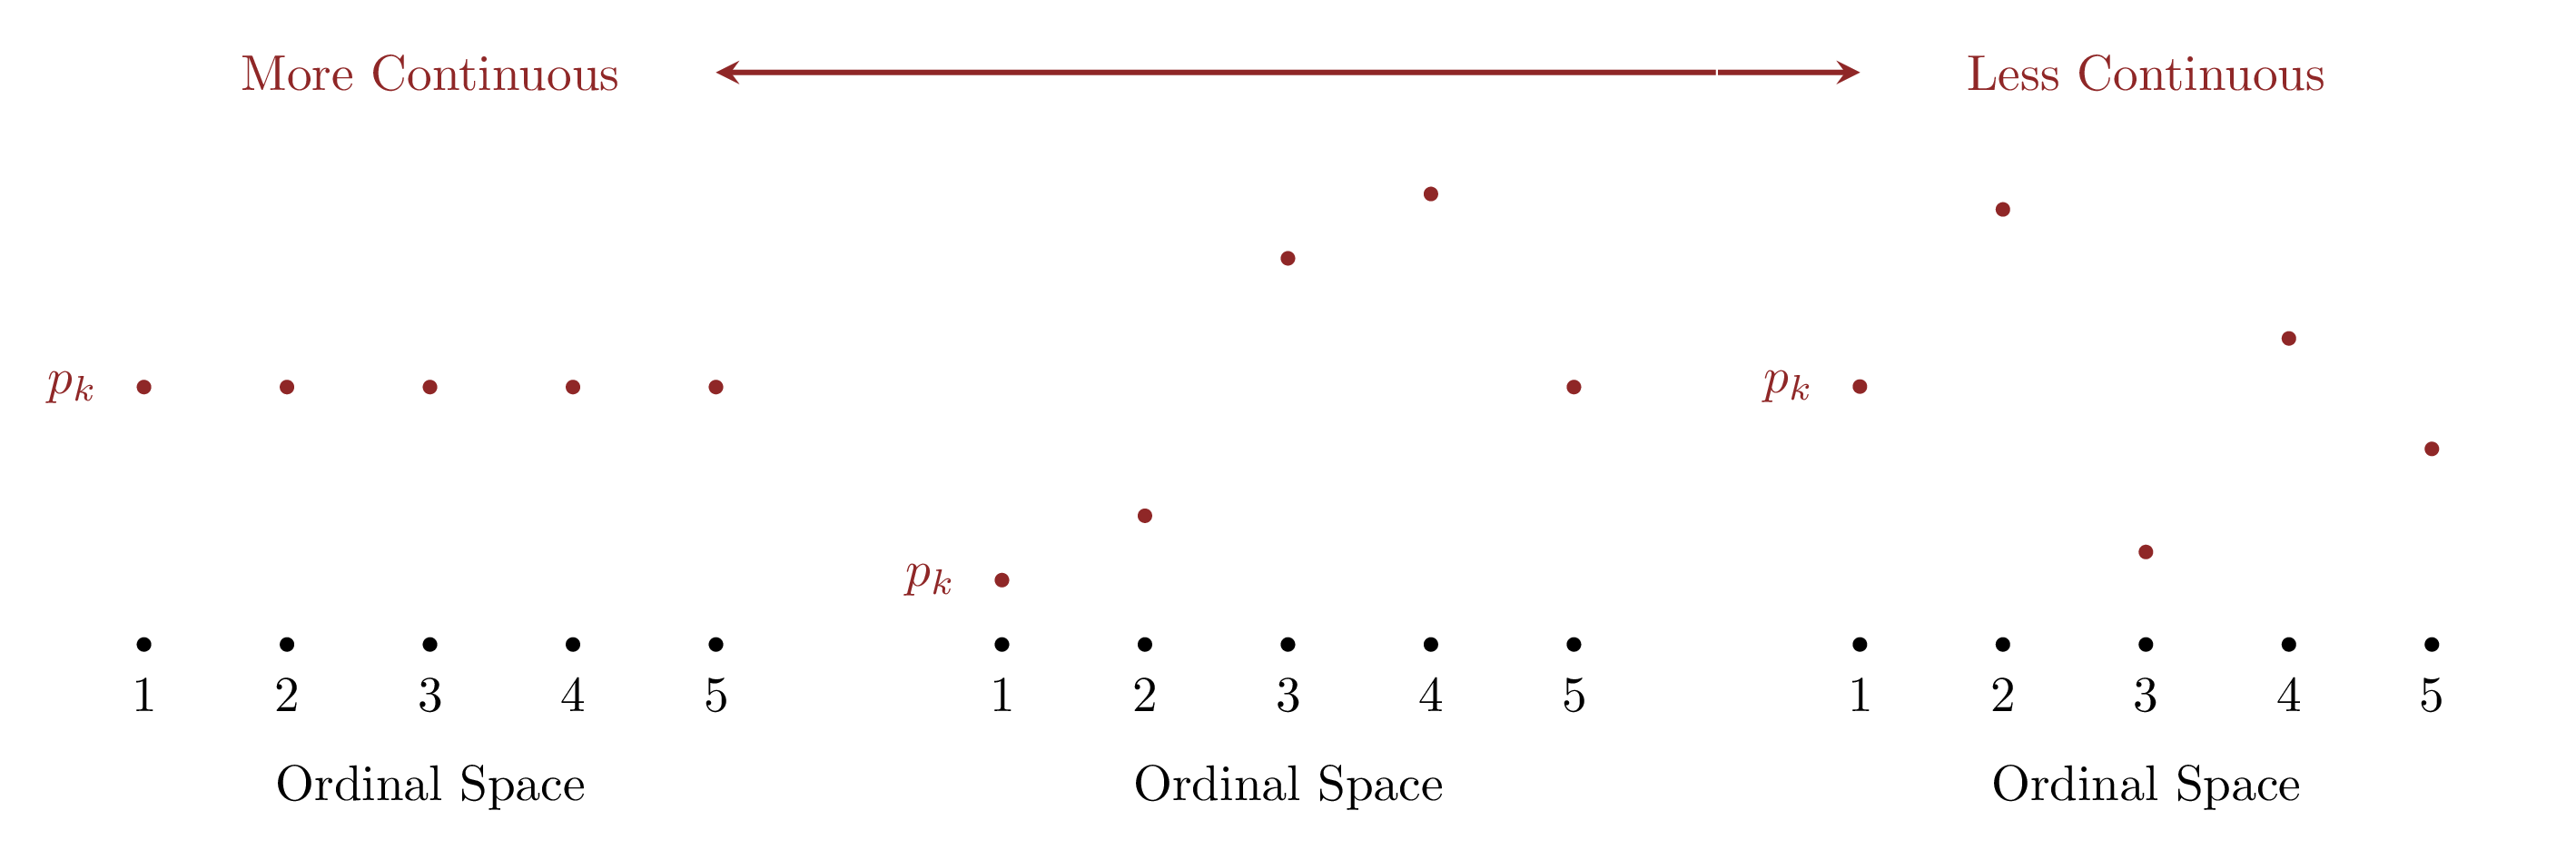
\includegraphics[width=1\textwidth,height=\textheight]{figures/continuity/continuity.png}

}

\caption{\label{fig-continuity}In a categorical model any ordering of
the elements is arbitrary and we consequently cannot define even a
qualitative notion of continuous probability allocations. Ordinal
spaces, however, are equipped with a distinguished ordering that defines
neighboring elements and a vague notion of continuity where neighboring
probabilities are more similar than non-neighboring probabilities.}

\end{figure}%

Because notions of continuity on ordinal spaces are only qualitative,
however, it can be difficult to elicit appropriate domain expertise in a
given application. When we are not able to elicit precise constraints
then there's no real loss from ignoring the ordering and using a
categorical model.

Moreover in circumstances where we do have quantified domain expertise
it can often be implemented with a simple categorical model complemented
by an informative prior model. In particular if our domain expertise
manifests as a preference for probabilities that vary around a baseline
simplex configuration \(\boldsymbol{\rho}\) then we could use a
Dirichlet prior model with the configuration
(Figure~\ref{fig-dirichlet}) \[
\alpha_{k} = \rho_{k} / \tau + 1.
\]

\begin{figure}

\centering{

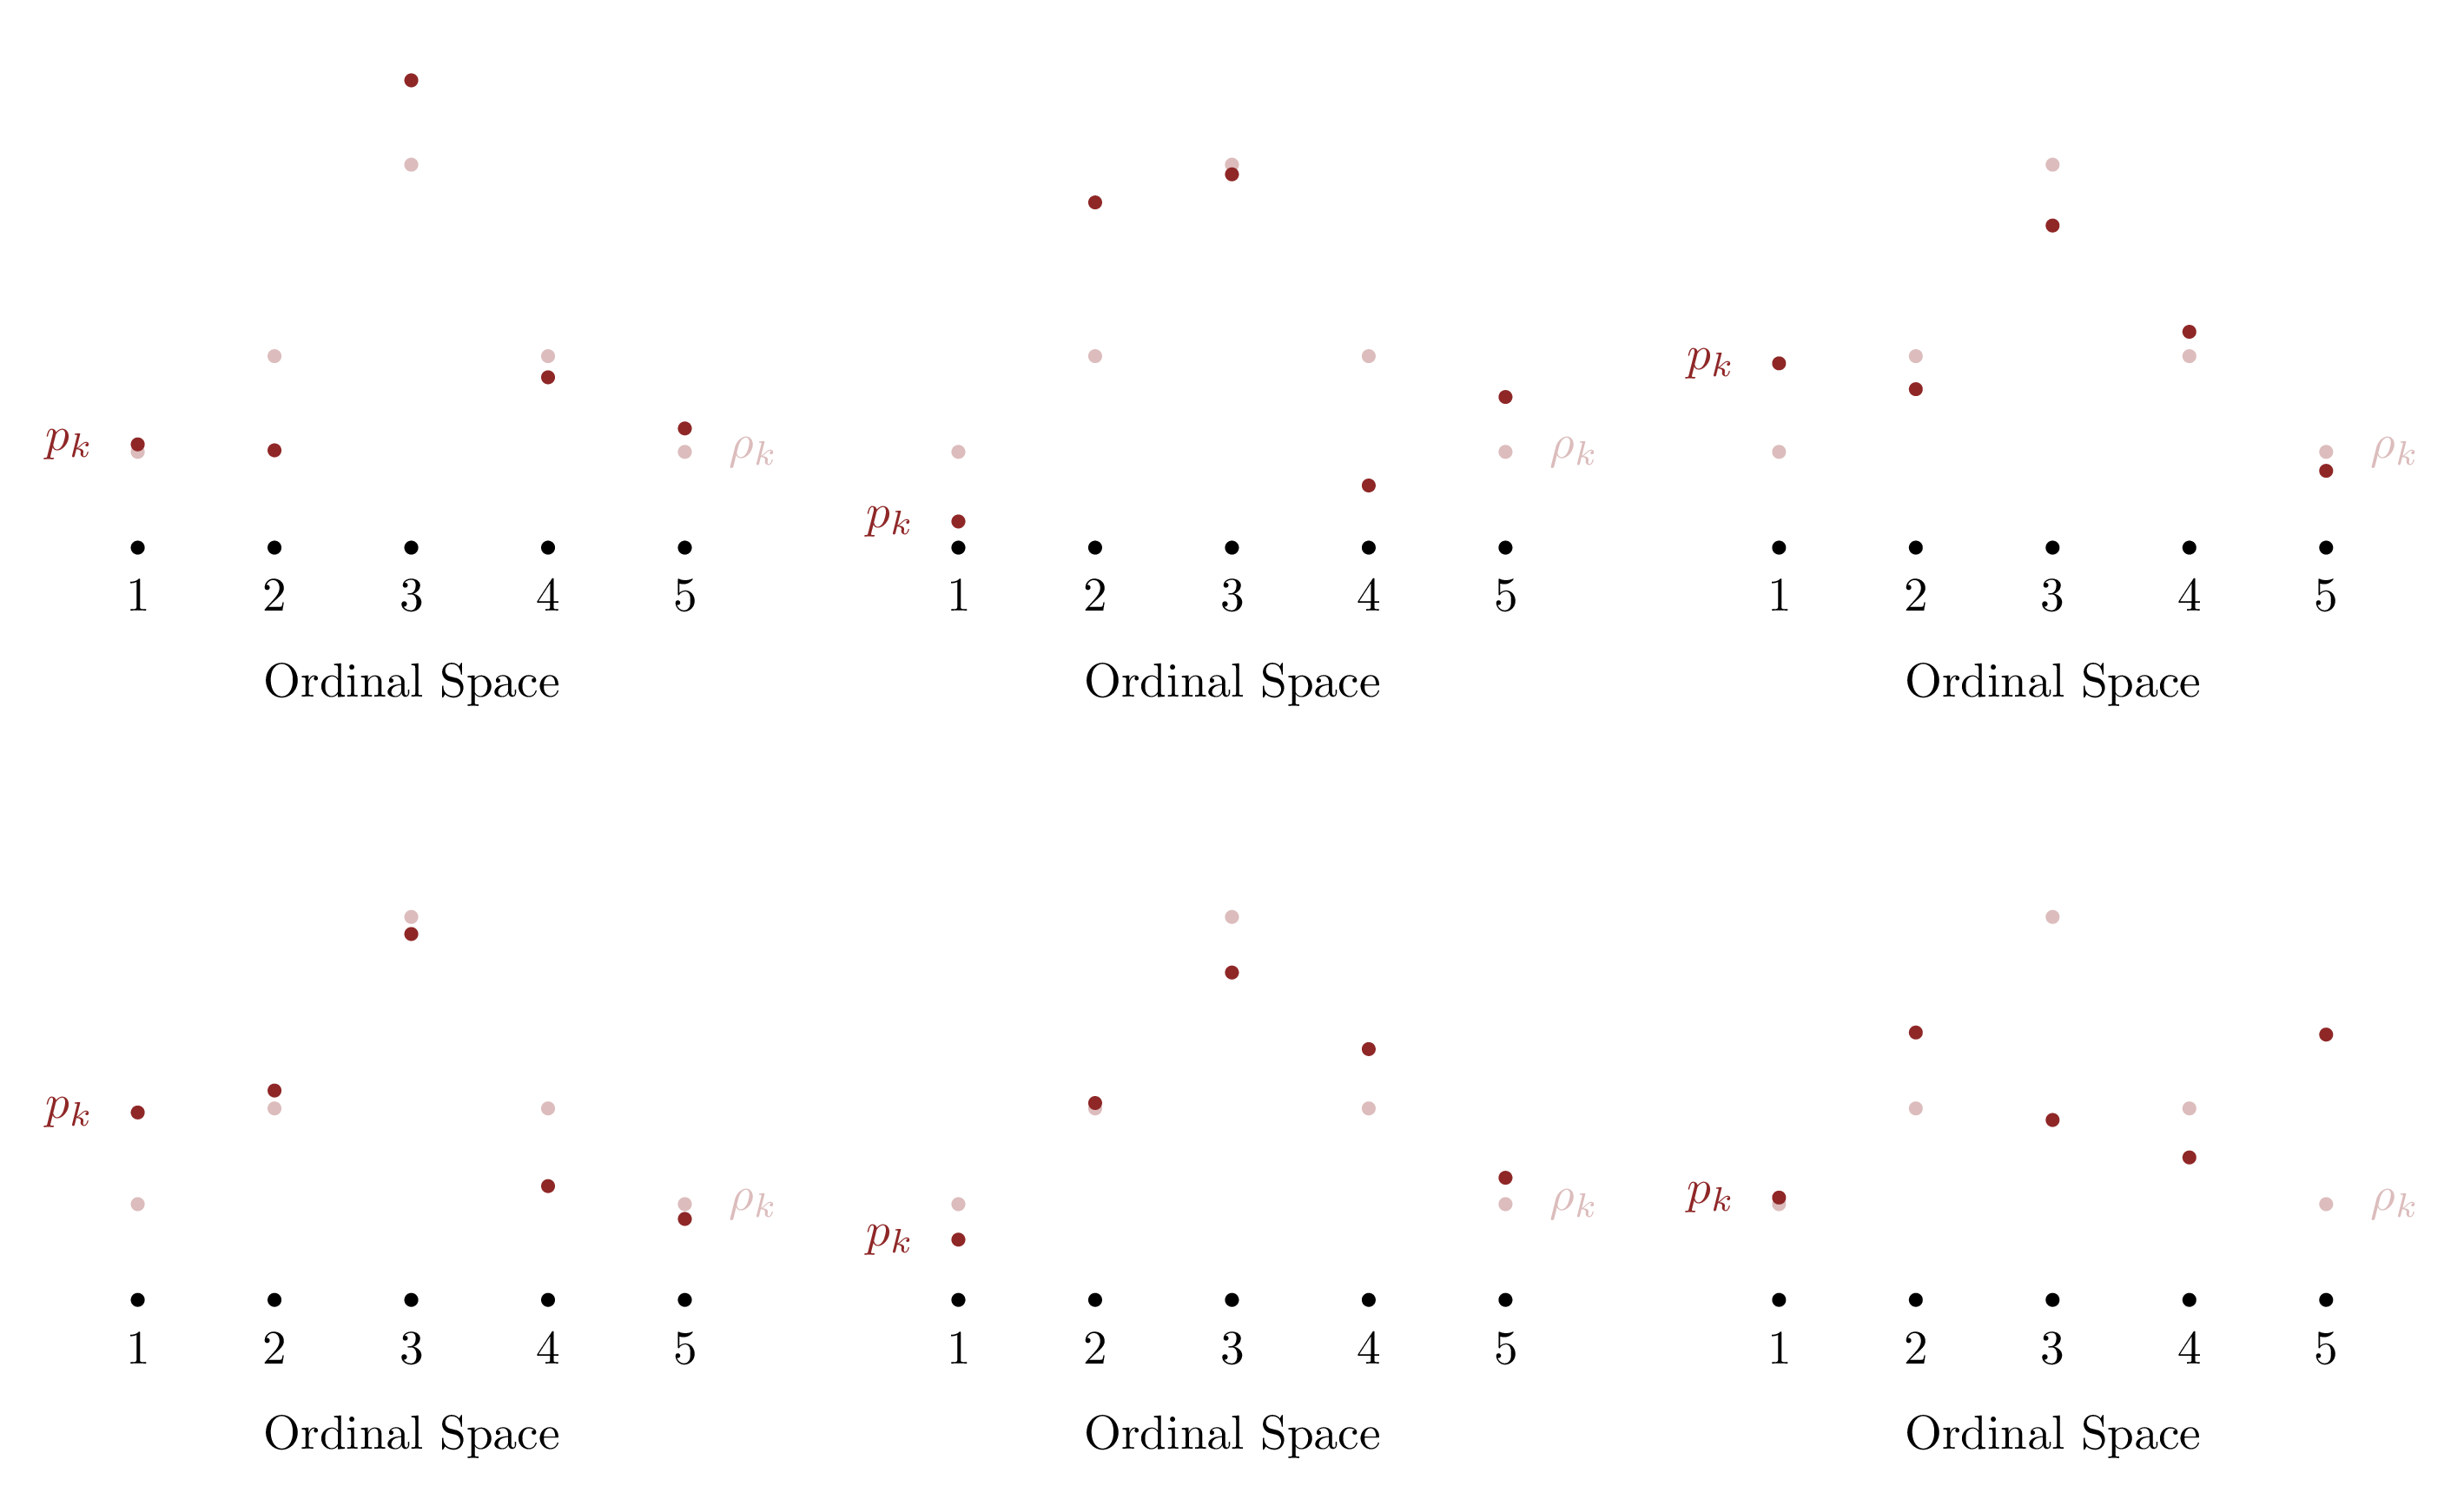
\includegraphics[width=1\textwidth,height=\textheight]{figures/dirichlet/dirichlet.png}

}

\caption{\label{fig-dirichlet}A Dirichlet prior model with the
configuration parameters \(\alpha_{k} = \rho_{k} / \tau + 1\)
concentrates around the baseline simplex configuration
\((\rho_{1}, \ldots, \rho_{K})\), here shown in light red. Samples from
this prior model, here shown in dark red, cluster around this baseline
and preserve its basic shape.}

\end{figure}%

Even vague notions of continuity can become a much more relevant
consideration when we are modeling \emph{heterogeneity} in ordinal
probabilities. Specifically we often want whatever shape that happens to
manifest in the ordinal probabilities of some \emph{baseline}
circumstance to be somewhat preserved in the other circumstances. In
other words the problem of interest is often not modeling independent
ordinal probabilities but rather modeling \emph{systematic
perturbations} of the baseline ordinal probabilities
(Figure~\ref{fig-perturbed-probs}).

\begin{figure}

\centering{

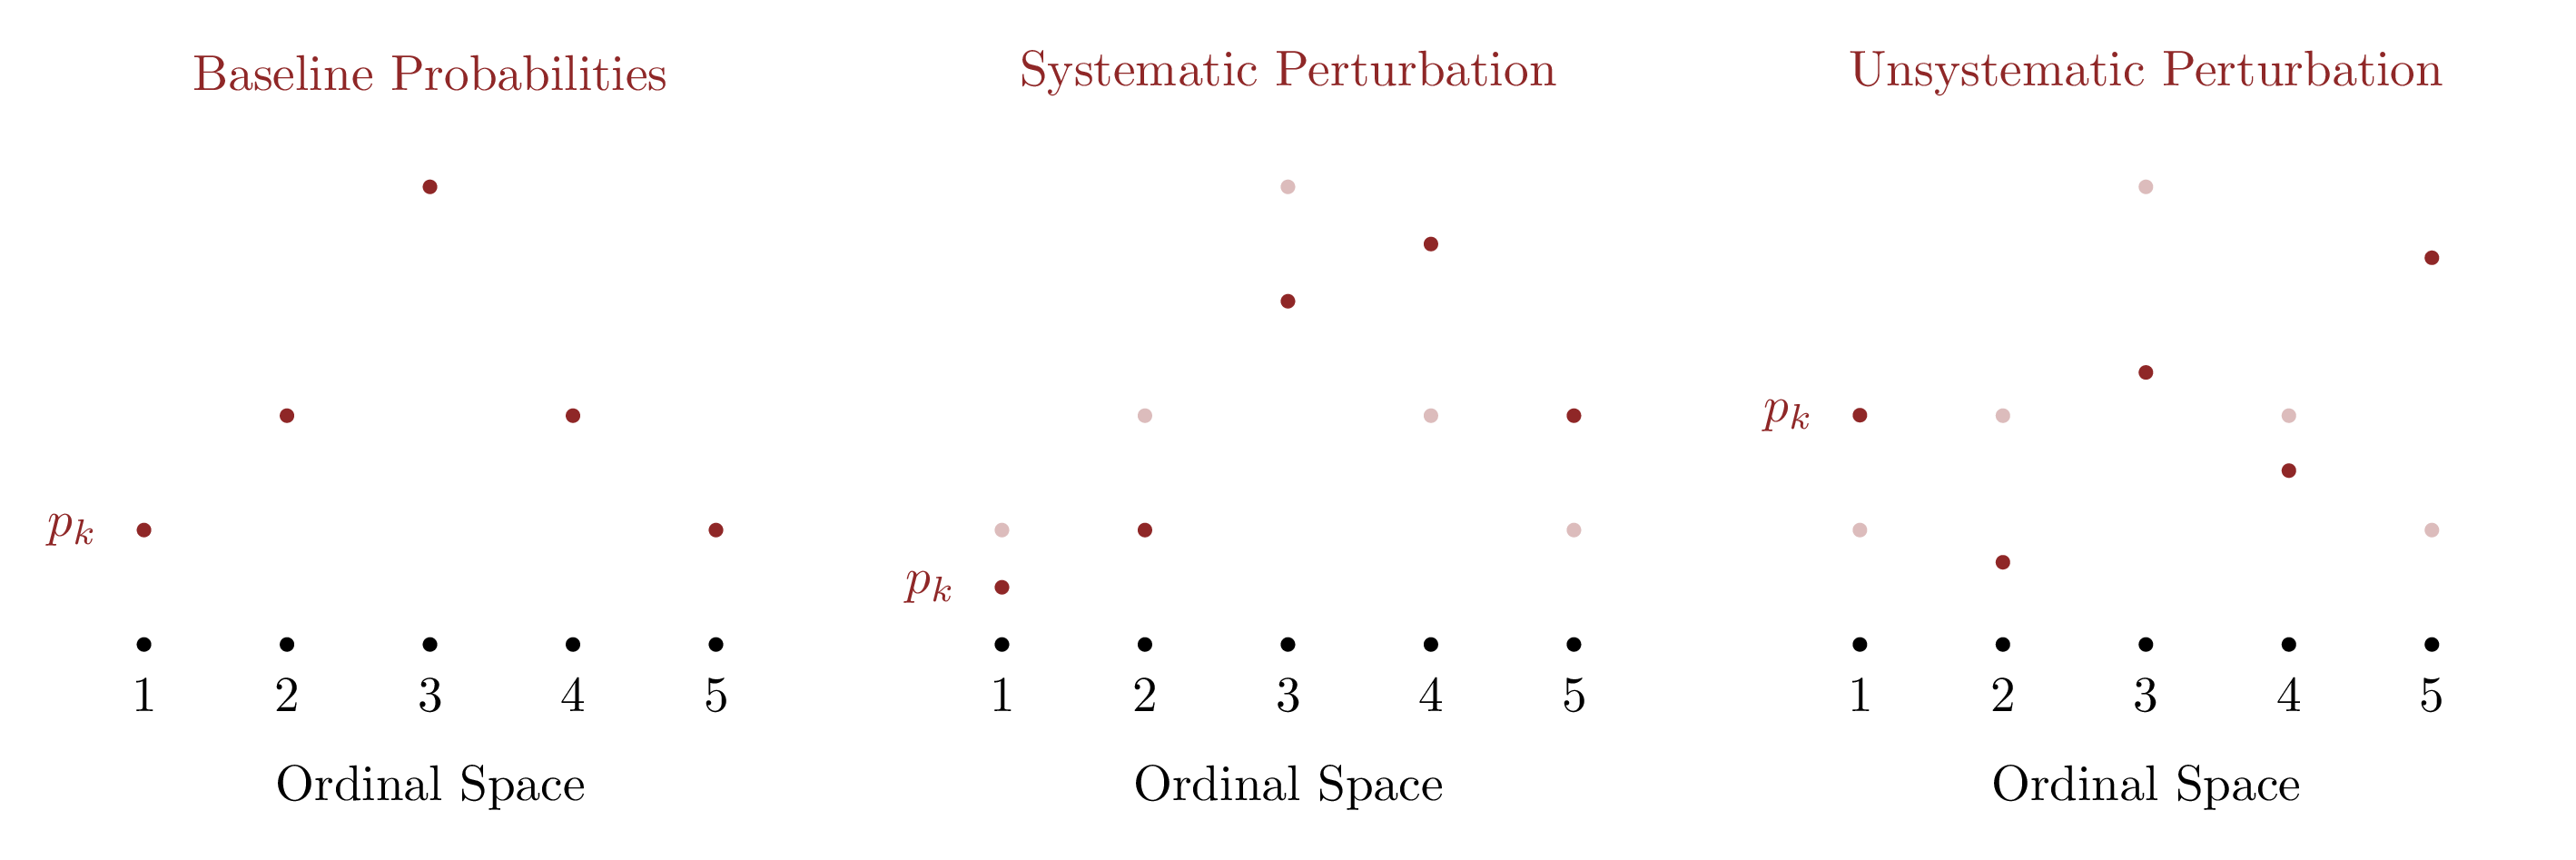
\includegraphics[width=1\textwidth,height=\textheight]{figures/perturbed_probs/perturbed_probs.png}

}

\caption{\label{fig-perturbed-probs}Heterogeneous ordinal probabilities
can always be modeled independently of each other. In many applications,
however, our domain expertise is consistent with more systematic
variations around some baseline behavior. This raises the question of
how we can build ordinal models that isolate the relevant variations.}

\end{figure}%

\section{Coupling Ordinal
Probabilities}\label{coupling-ordinal-probabilities}

One of the most effective ways to limit the behavior of ordinal
probabilities is not to model them directly but rather to \emph{derive}
them from a latent probability space that is already equipped with a
more manageable form of continuity.

\subsection{Discretizing A Continuous Probability
Space}\label{derived-probs}

Continuity of behaviors is much easier to quantify on continuous spaces.
In particular let's consider a real line \(X = \mathbb{R}\) equipped
with a probability distribution \(\pi\) specified by the probability
density function \(p : X \rightarrow \mathbb{R}^{+}\).

Any partition of \(X\) is defined by a sequence of disjoint but
connected intervals, \begin{align*}
I_{1} &= (-\infty, c_{1} ]
\\
&= \ldots
\\
I_{k} &= ( c_{k - 1}, c_{k} ]
\\
&= \ldots
\\
I_{K} &= ( c_{K - 1}, +\infty ).
\end{align*} Together these intervals define a finite space \[
( I_{1}, \ldots, I_{k}, \ldots, I_{K} ).
\] Moreover because all points in one interval are strictly less than or
larger than all of the points in any other interval, \[
x < x'
\] for all \(x \in I_{k}\) and \(x' \in I_{k' > k}\), these elements are
naturally ordered, \[
I_{k} < I_{k' > k}.
\] Consequently the set of intervals is an ordinal space.

The boundaries between these intervals \[
c_{0} = -\infty
< c_{1}
< \ldots
< c_{k}
< \ldots
< c_{K - 1}
< c_{K} = +\infty
\] are known as \textbf{cut points} as they, well, cut the real line
into pieces. I will refer to the \(K - 1\) points \[
-\infty < c_{1} < \ldots < c_{k} < \ldots < c_{K - 1} < +\infty
\] as \textbf{interior cut points}.

Now that we can map a real line to a \(K\) element ordinal space we can
push the latent probability distribution forward to ordinal
probabilities. In particular the probability allocated to each ordinal
element is the probability allocated to the defining interval
(Figure~\ref{fig-interval-probs}), \[
p_{k}
= \pi( \, ( c_{k - 1}, c_{k} ] \, )
= \int_{c_{k - 1}}^{c_{k}} \mathrm{d} x' \, p(x').
\]

\begin{figure}

\centering{

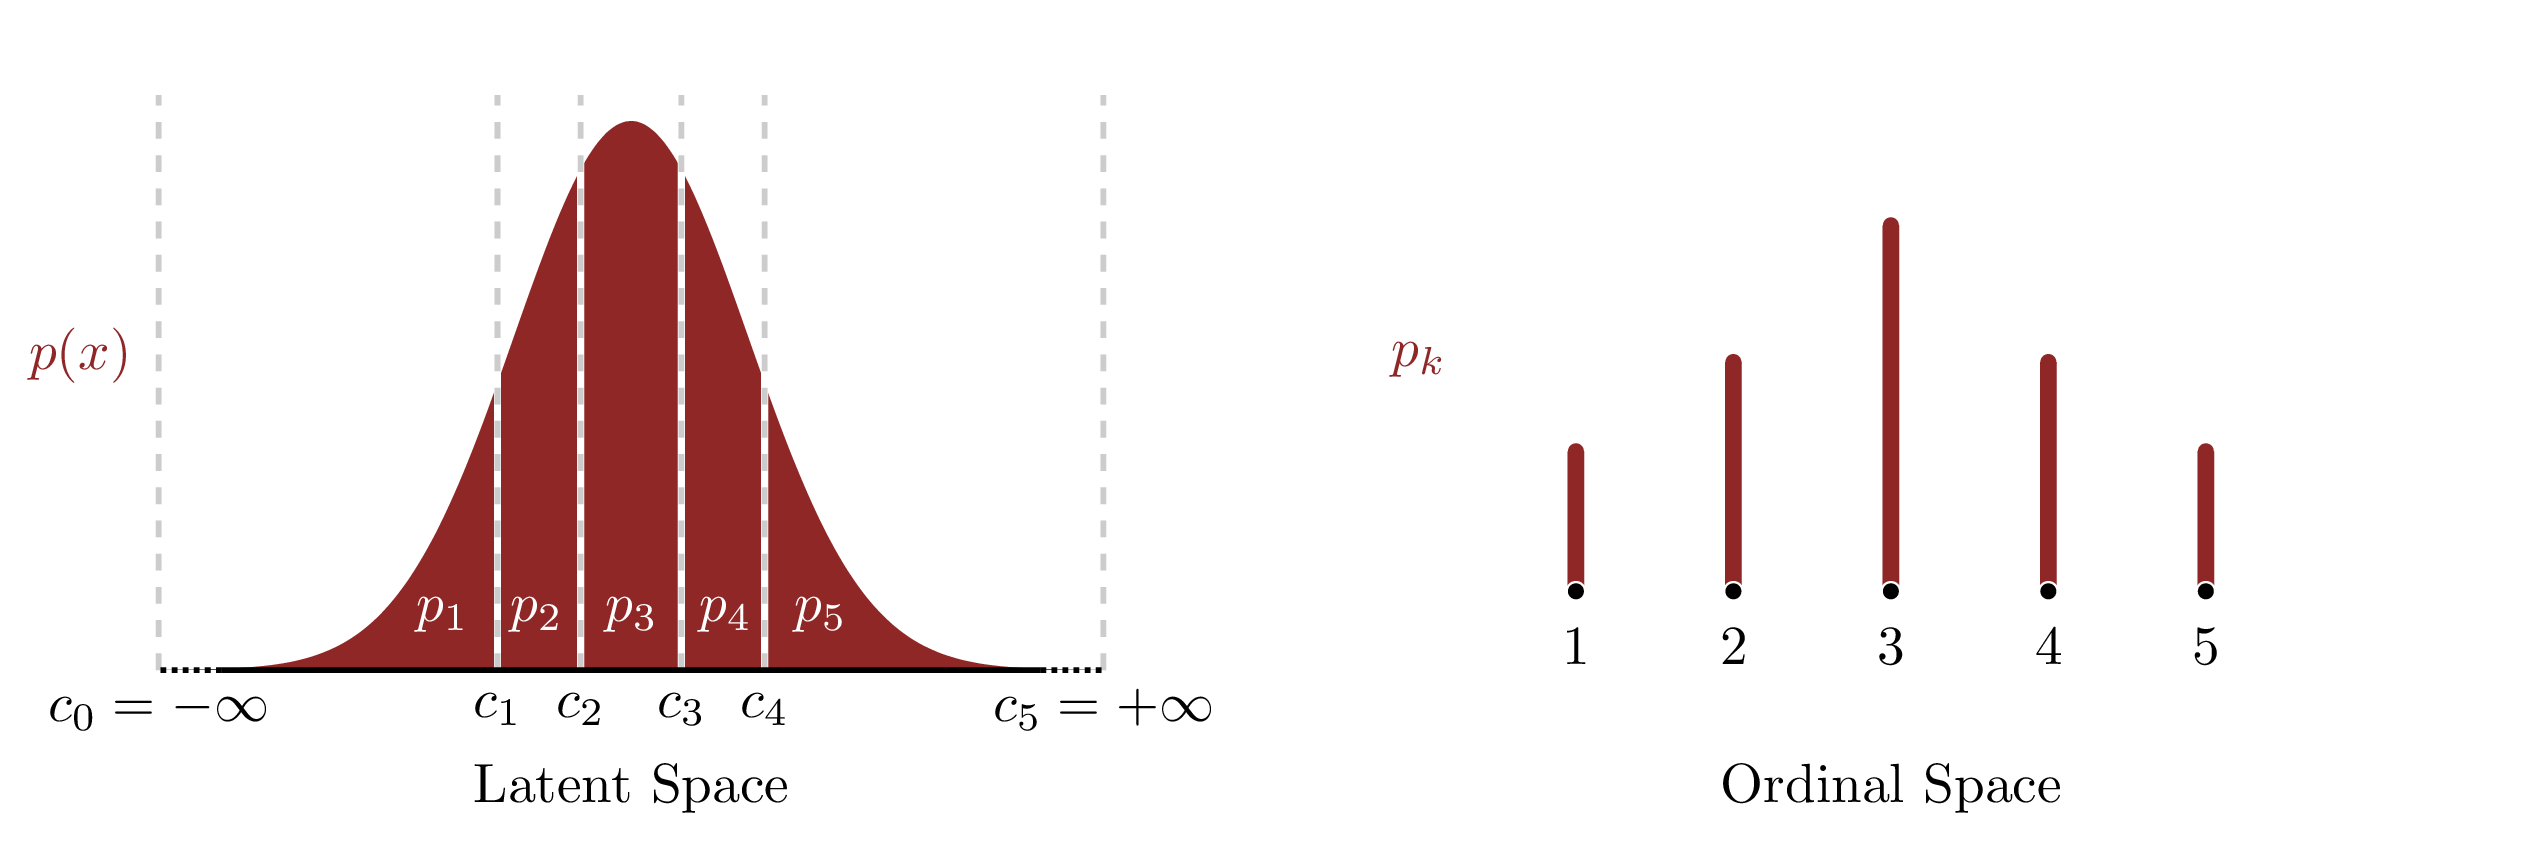
\includegraphics[width=0.9\textwidth,height=\textheight]{figures/interval_probs/interval_probs.png}

}

\caption{\label{fig-interval-probs}Cut points partition a latent real
line into ordered intervals which defines an ordinal space. They also
partition a latent probability density function into interval
probabilities which defines a probability distribution over that ordinal
space.}

\end{figure}%

Given a cumulative distribution function \[
\Pi(x) = \int_{-\infty}^{x} \mathrm{d} x' \, p(x')
\] we can equivalently calculate the derived ordinal probabilities as
(Figure~\ref{fig-cdf-calcs}) \[
p_{k} = \Pi(c_{k}) - \Pi(c_{k - 1}).
\] If the cumulative distribution function is available in closed form
then this form allows us to quickly compute the ordinal probabilities
with just a few subtractions.

\begin{figure}

\centering{

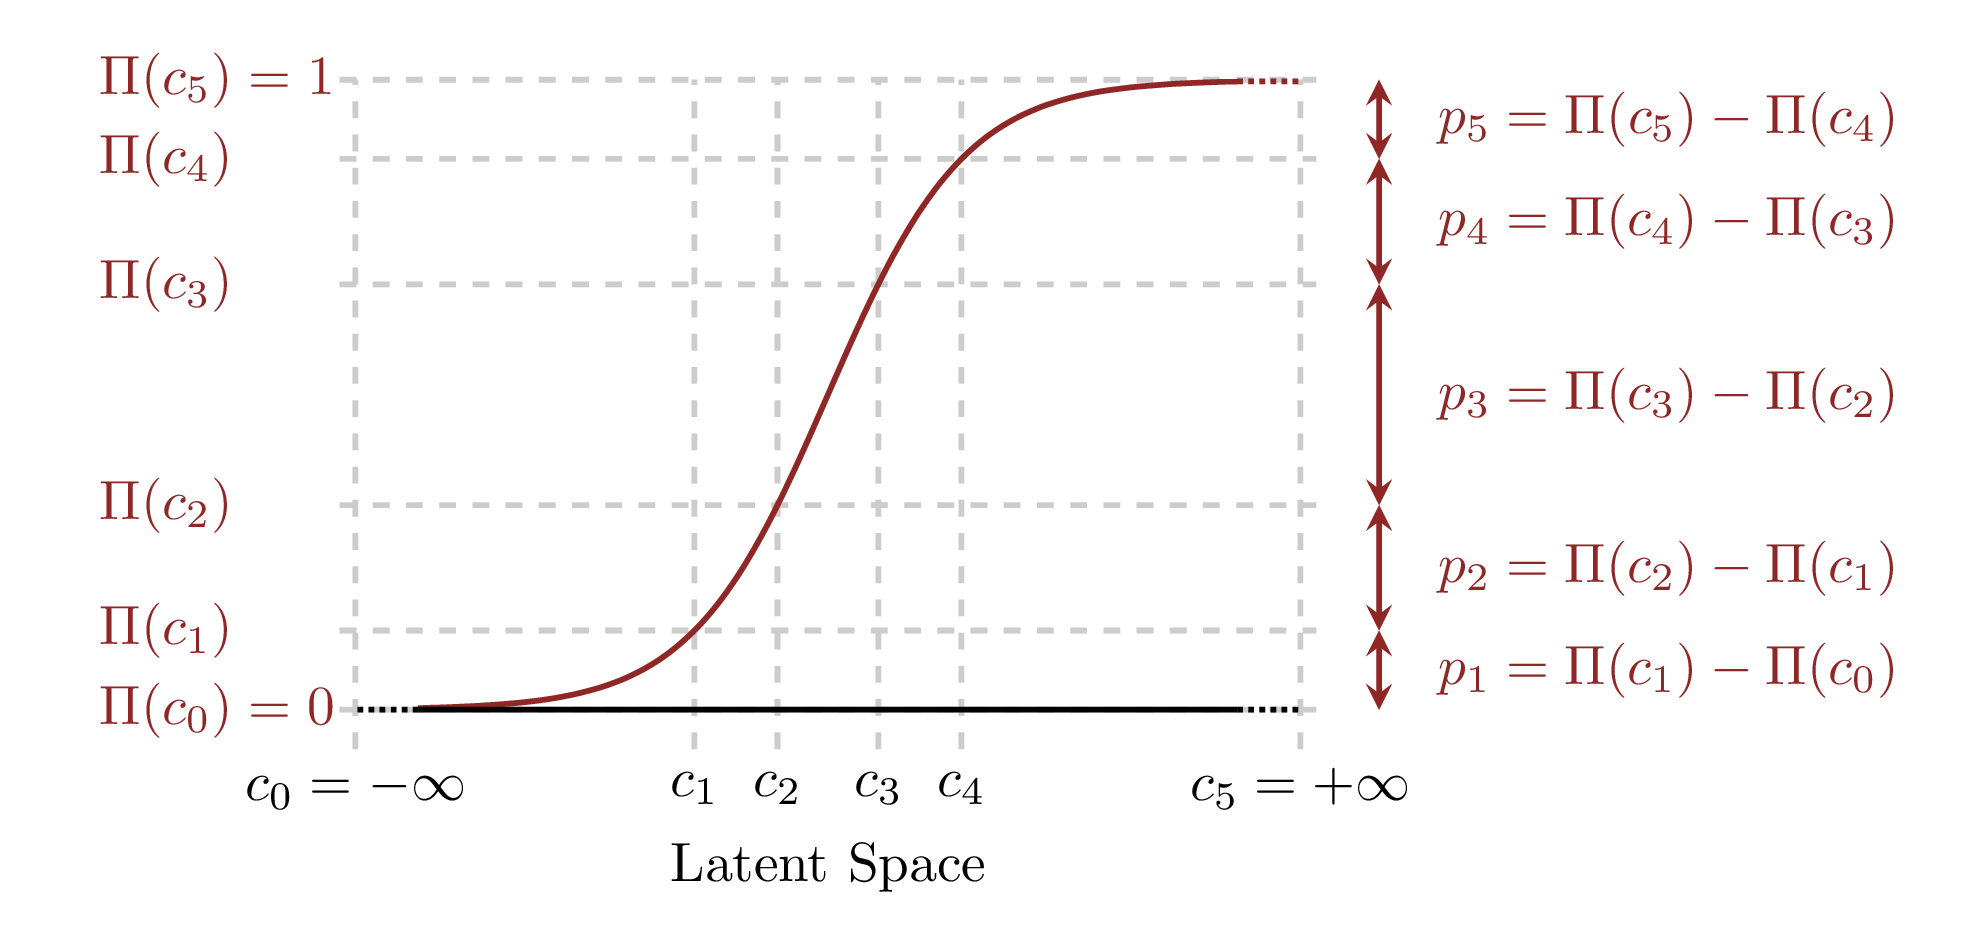
\includegraphics[width=0.75\textwidth,height=\textheight]{figures/cdf_calcs/cdf_calcs.png}

}

\caption{\label{fig-cdf-calcs}We can quickly compute interval
probabilities, and hence induced ordinal probabilities, by subtracting
cumulative distribution functions.}

\end{figure}%

For any probability distribution on a real line we have \begin{align*}
\Pi(-x)
&=
\int_{-\infty}^{-x} \mathrm{d} x' \, p(x')
\\
&=
-\int_{+\infty}^{x} \mathrm{d} x'' \, p(x'')
\\
&=
\int_{x}^{\infty} \mathrm{d} x'' \, p(x'')
\\
&=
1 - \int_{-\infty}^{x} \mathrm{d} x'' \, p(x'')
\\
&=
1 - \Pi(x).
\end{align*} Consequently we can also write the ordinal probabilities as
(Figure~\ref{fig-ccdf-calcs}) \begin{align*}
p_{k}
&=
\Pi(c_{k}) - \Pi(c_{k - 1})
\\
&=
\big( \Pi(c_{k}) - 1 \big) - \big( \Pi(c_{k - 1}) - 1 \big)
\\
&=
- \big( 1 - \Pi(c_{k}) \big) + \big( 1 - \Pi(c_{k - 1}) \big)
\\
&=
- \Pi(-c_{k}) + \Pi(-c_{k - 1})
\\
&=
\Pi(-c_{k - 1}) - \Pi(-c_{k}).
\end{align*} This equivalent form is more common in some references.

\begin{figure}

\centering{

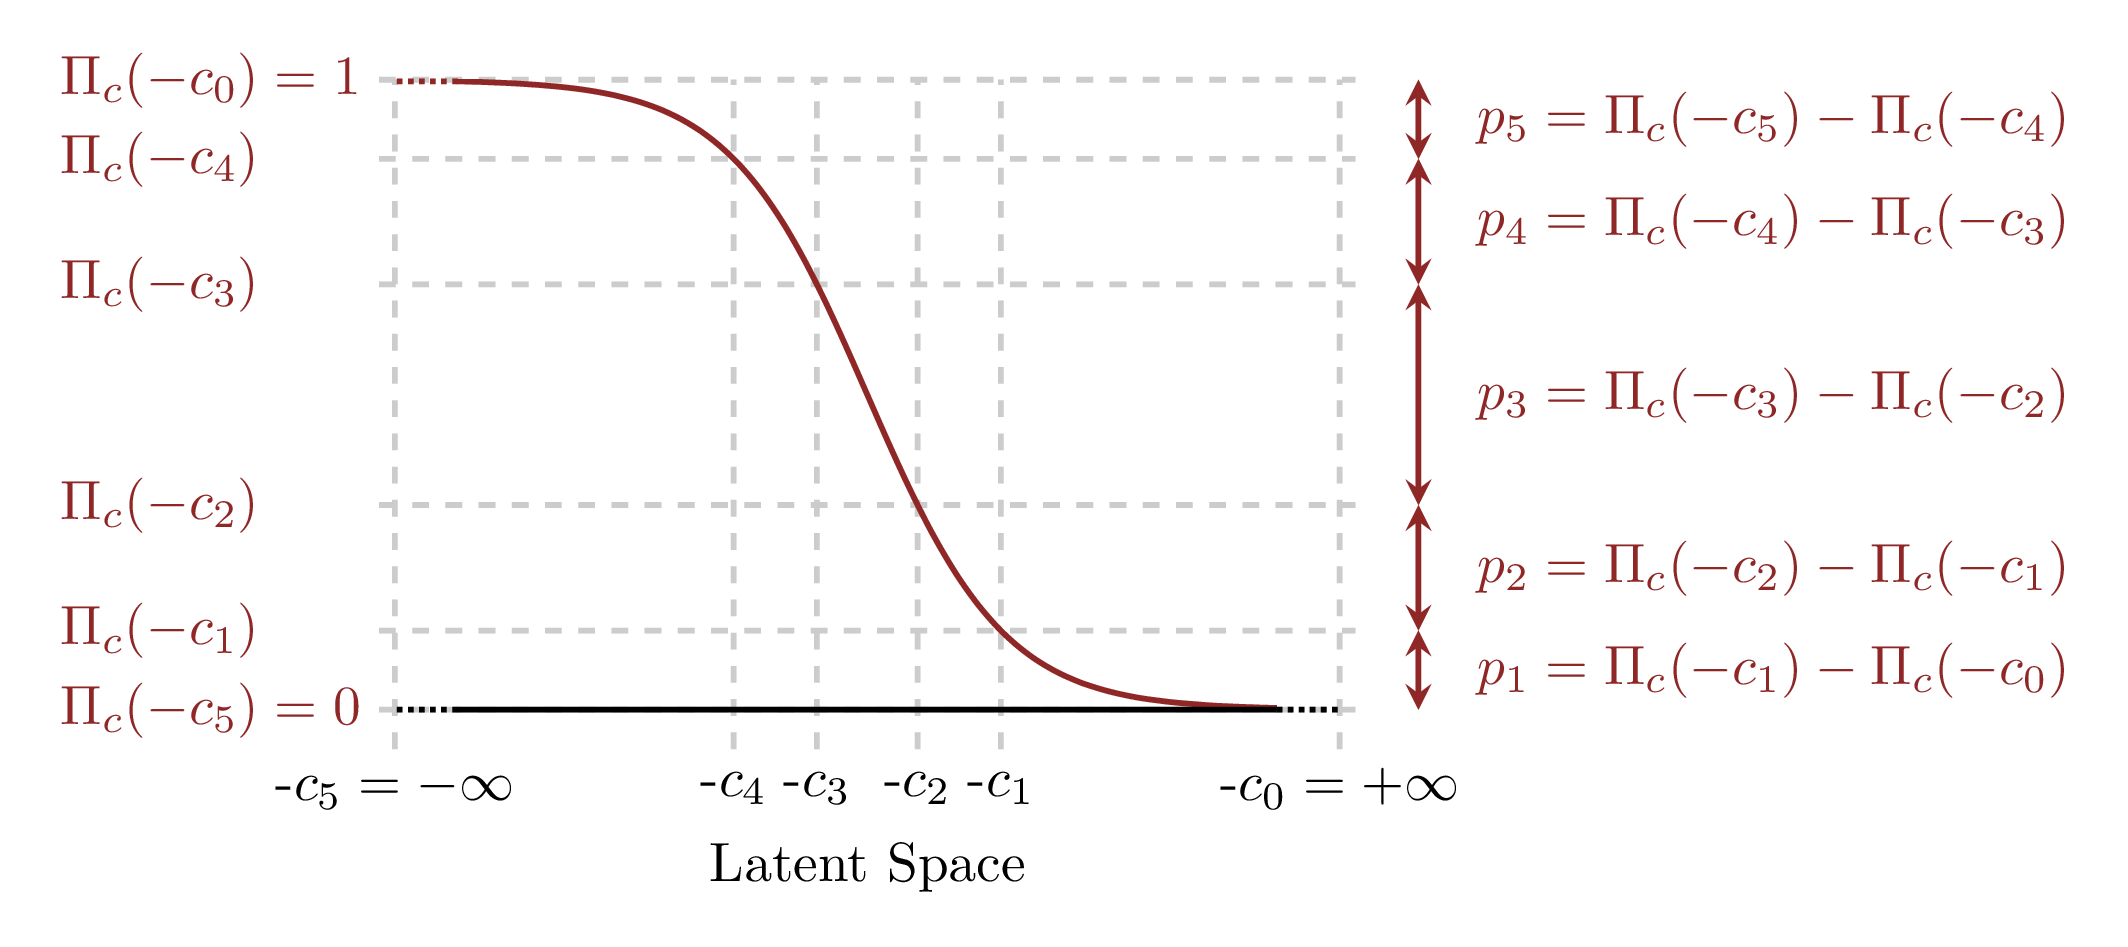
\includegraphics[width=0.75\textwidth,height=\textheight]{figures/ccdf_calcs/ccdf_calcs.png}

}

\caption{\label{fig-ccdf-calcs}Interval probabilities can also be
written as differences of complementary cumulative distribution
functions \(\Pi_{c}(x) = 1 - \Pi(x)\) provided we also negate the cut
points.}

\end{figure}%

\subsection{The Duality Between Cut Points and Ordinal
Probabilities}\label{sec:duality}

If the distances between the interior cut points are similar then the
resulting ordinal probabilities will manifest the basic shape of the
latent probability density function. In particular the more rigid the
latent probability density function is the more similar probabilities
allocated to neighboring intervals will tend to be relative to the
allocations to non-neighboring intervals.

That said if the configuration of the interior cut points, and the
lengths of the intervals between them, is arbitrary then the resulting
ordinal probabilities will also be arbitrary \emph{regardless of the
shape of the latent probability density function}. More formally for
\emph{any} fixed latent probability density function we have a bijection
between the interior cut points and the first \(K - 1\) ordinal
probabilities, with the last ordinal probability then given by the
simplex constraint, \[
p_{K} = 1 - \sum_{k' = 1}^{K - 1} p_{k'}.
\]

We've already constructed the map from interior cut points to the first
\(K - 1\) ordinal probabilities, \[
p_{k}
=
\left\{
\begin{array}{rr}
\Pi(c_{k}), & k = 1 \\
\Pi(c_{k}) - \Pi(c_{k - 1}), & 1 \le k \le K - 1
\end{array}
\right. .
\] The inverse mapping is straightforward once we recognize that if we
sum over the first \(k' < K\) ordinal probabilities then most of the
cumulative distribution functions cancel, \[
\sum_{k' = 1}^{k} p_{k'}
=
\sum_{k' = 1}^{k} \Pi(c_{k'}) - \Pi(c_{k' - 1})
=
\Pi(c_{k}).
\] Consequently the \(k\)th interior cut point can be derived from the
first \(k\) ordinal probabilities, \[
c_{k} = \Pi^{-1} \left( \sum_{k' = 1}^{k} p_{k'} \right).
\]

\begin{figure}

\centering{

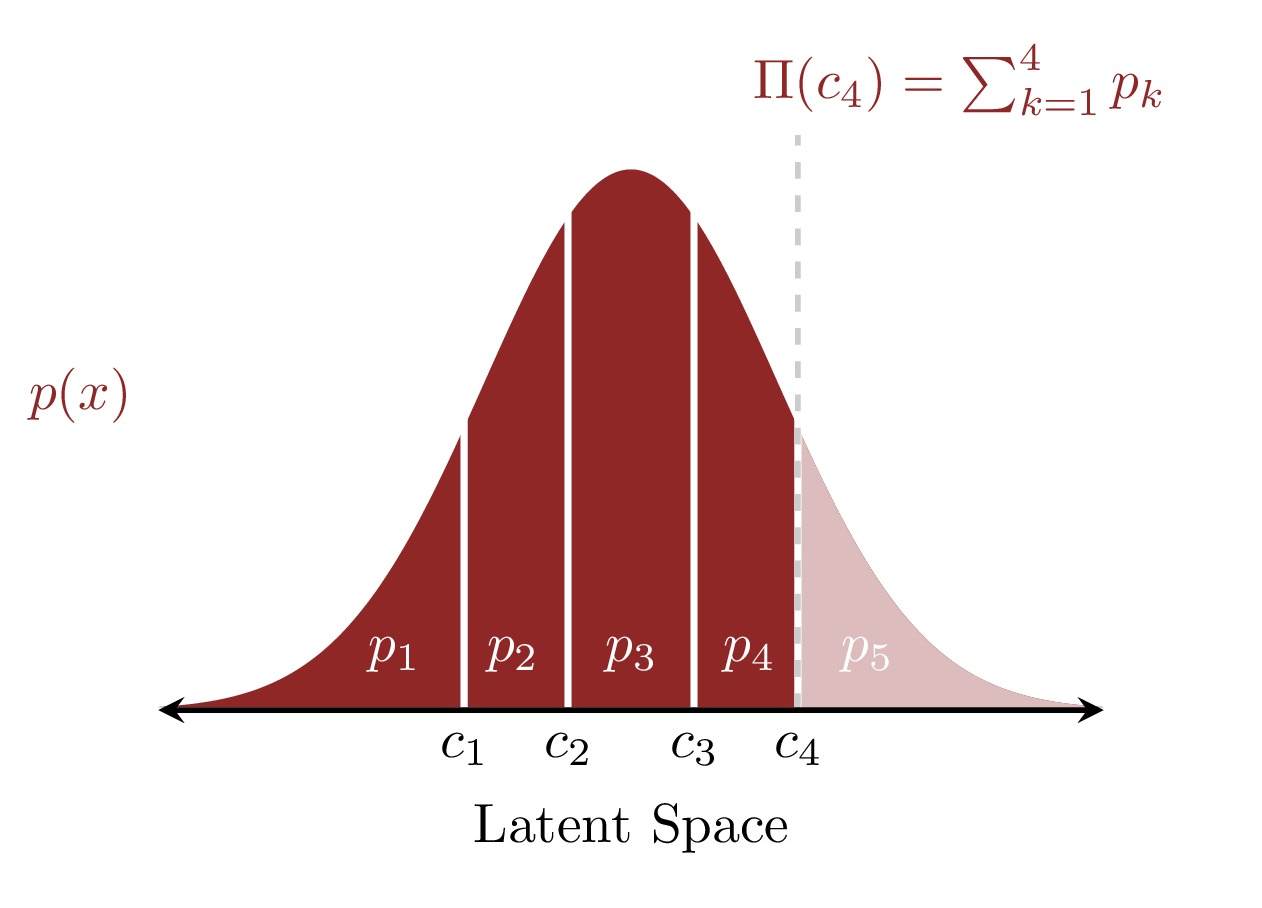
\includegraphics[width=0.6\textwidth,height=\textheight]{figures/inverse/inverse.png}

}

\caption{\label{fig-inverse}The cumulative distribution function
evaluated at the \(k\)th cut point \(c_{k}\) is always the sum of the
first \(k\) ordinal probabilities. Consequently we can compute any cut
point by summing the appropriate ordinal probabilities and then
inverting the cumulative distribution function.}

\end{figure}%

In fact this is really nothing more than the \textbf{stick-breaking} map
that is often used to unconstrained simplices in probabilistic
programming tools like Stan. Configuring the first interior cut point \[
c_{1} \in (-\infty, +\infty)
\] is equivalent to configuring the first break of the stick, \[
p_{1} \in [0, 1].
\] Similarly configuring the second interior cut point \[
c_{2} \in (c_{1}, +\infty)
\] is equivalent to the breaking the remaining stick, \[
p_{2} \in [ p_{1}, 1 ],
\] and so on, \[
c_{k} \in (c_{k - 1}, +\infty)
\Longleftrightarrow
p_{k} \in [p_{k - 1}, 1].
\]

Intuitively the interior cut points can \emph{always} reconfigure
themselves to compensate for any change in the latent probability
density function and recover any configuration of the ordinal
probabilities (Figure~\ref{fig-cut-point-flex}). Mechanically all we
have to do is swap out the cumulative distribution function and its
inverse. Consequently the ordinal probabilities will not, in general,
inherit the shape of the latent probability density function.

\begin{figure}

\centering{

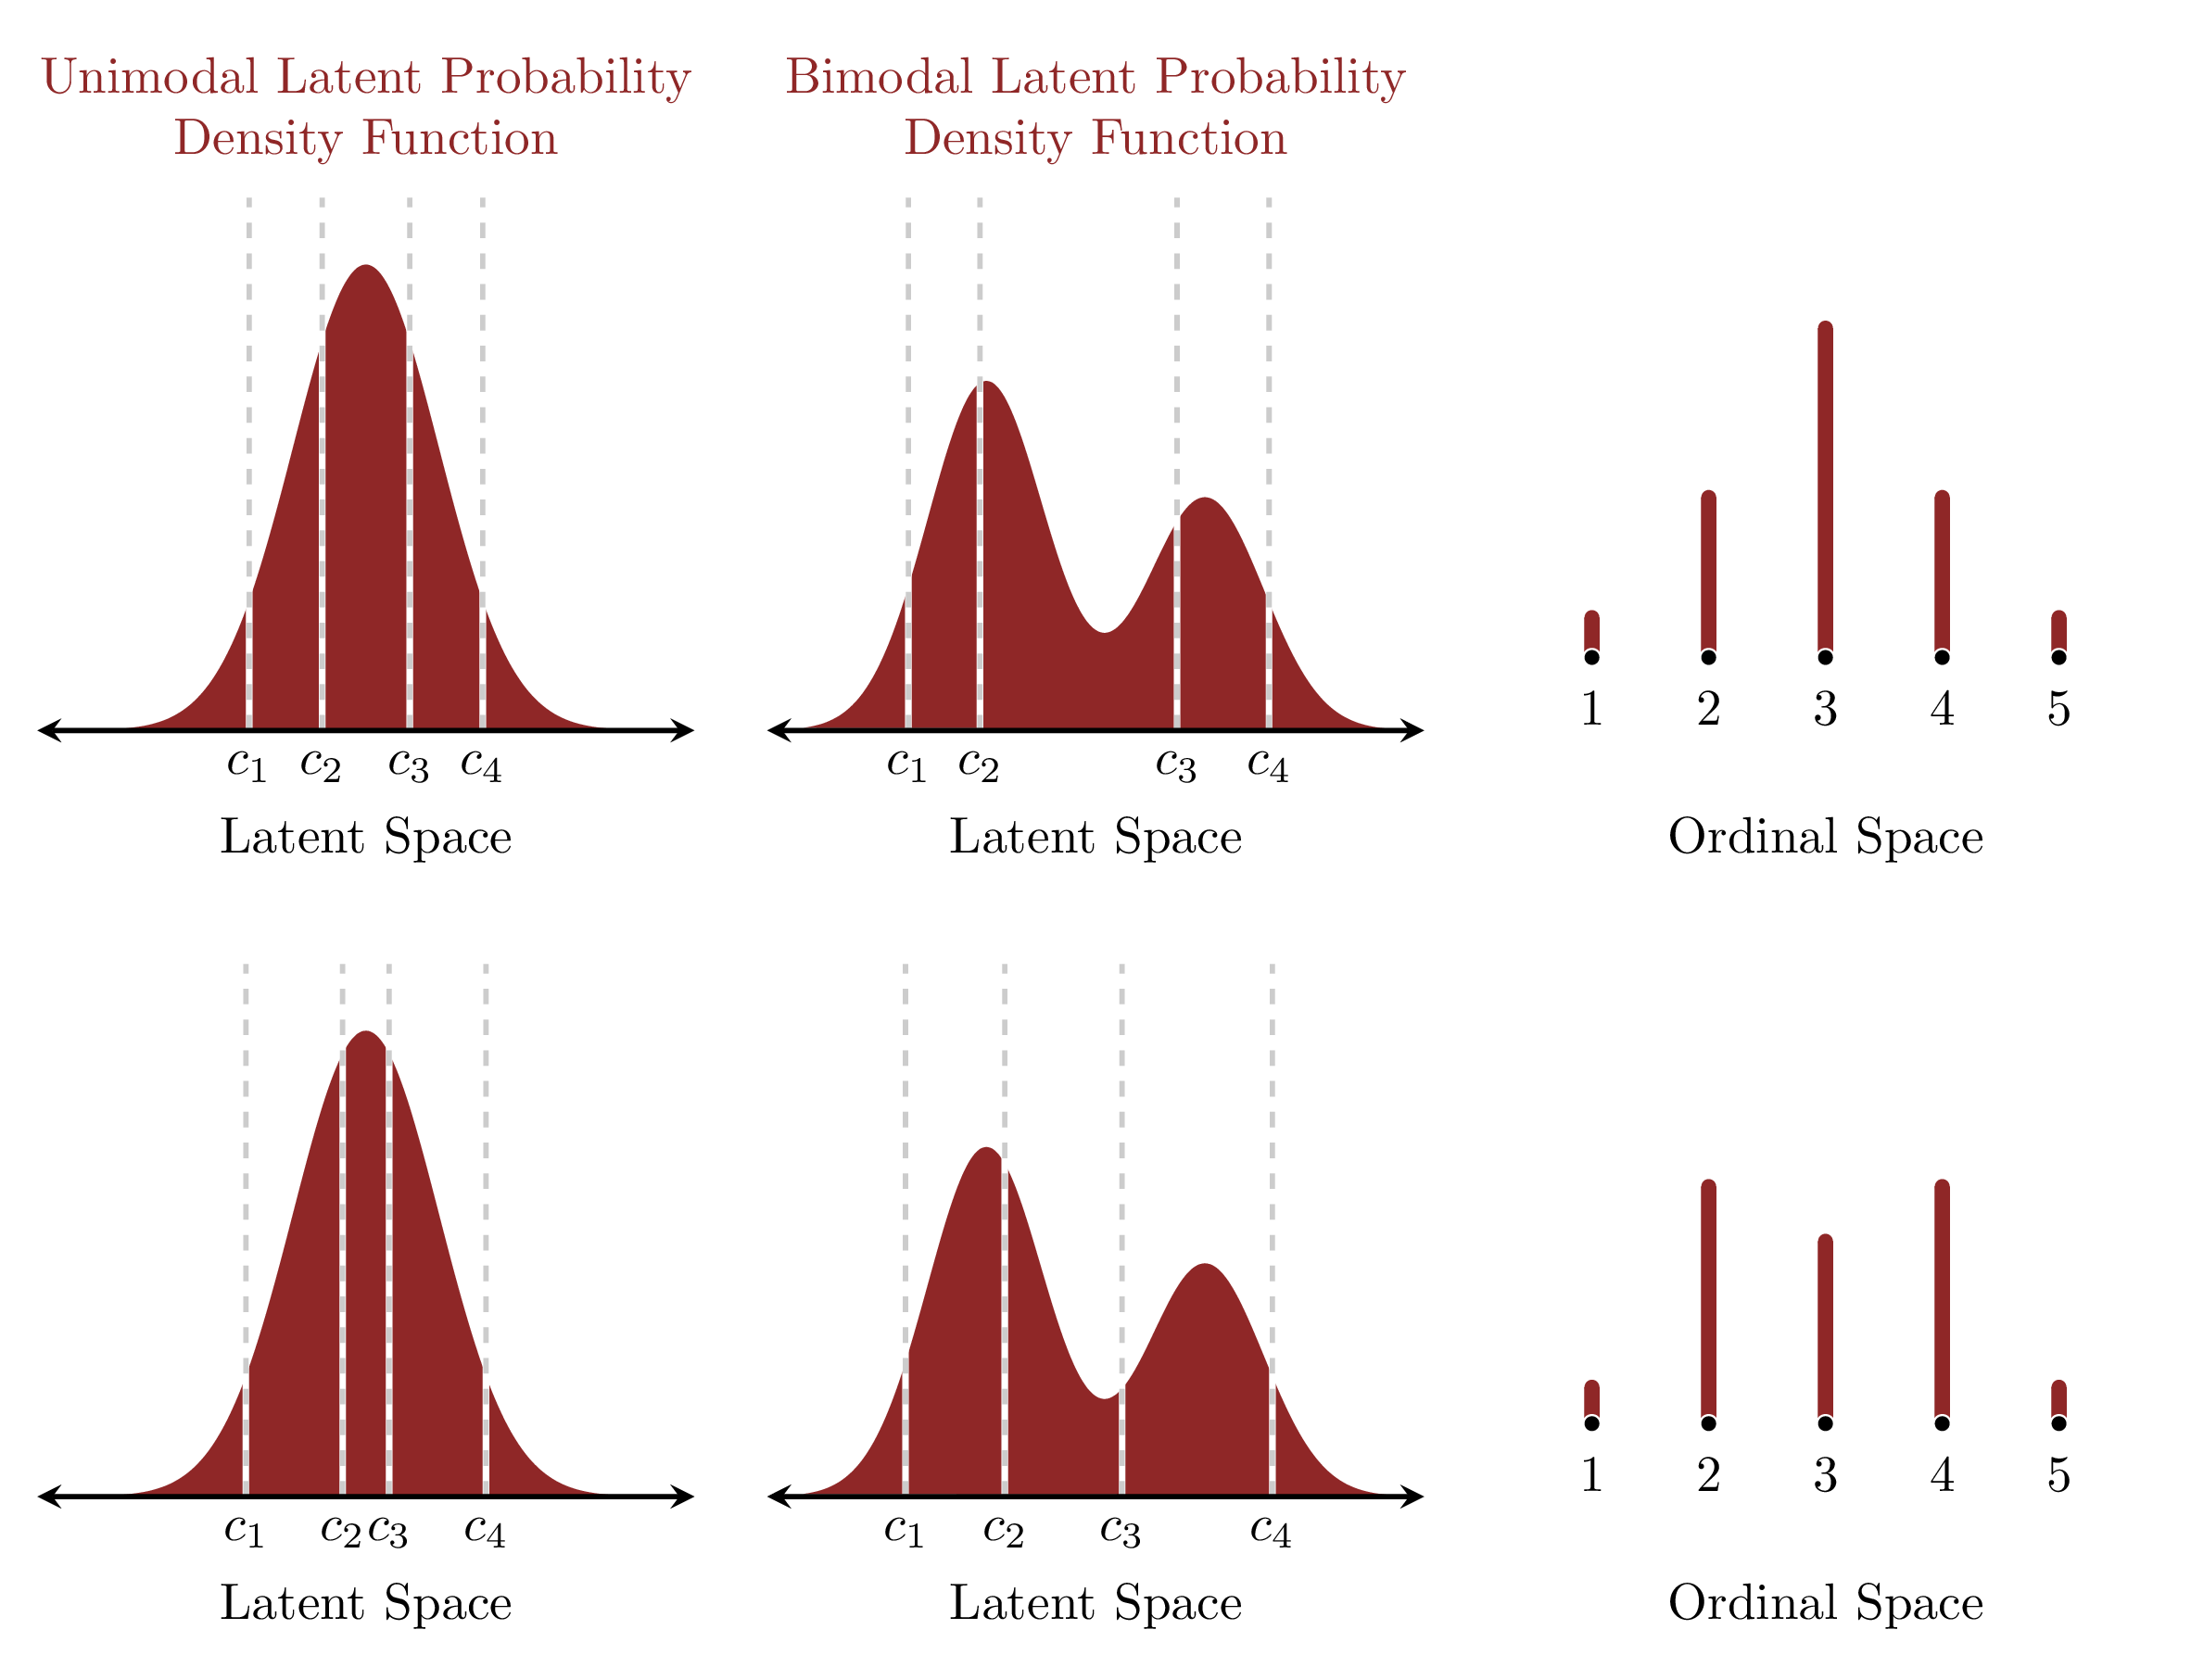
\includegraphics[width=1\textwidth,height=\textheight]{figures/cut_point_flex/cut_point_flex.png}

}

\caption{\label{fig-cut-point-flex}So long as the interior cut points
are unconstrained the cut point construction can recover any ordinal
probability configuration regardless of the shape of the latent
probability density function. For example both a unimodal and bimodal
latent probability density function can recover both unimodal and
bimodal ordinal probabilities.}

\end{figure}%

One immediate consequence of this duality is that so long as the
interior cut points are unconstrained we are free to choose a latent
probability density function that simplifies the implementation. For
example we can limit consideration to latent probability density
functions with both analytic cumulative distribution functions and
inverse cumulative distribution functions. Similarly we might make our
choice based on computational cost considerations.

Taking a logistic probability density function \[
\pi(x; \mu, \sigma)
=
\frac{1}{\sigma}
\frac{ \exp \left( - \frac{ x - \mu }{ \sigma } \right) }
{ \left( 1 + \exp \left( - \frac{ x - \mu }{ \sigma } \right) \right)^{2} }
\] with the cumulative distribution function \[
\pi(x; \mu, \sigma)
=
\frac{ 1 }{ 1 + \exp \left( - \frac{ x - \mu }{ \sigma } \right) }
\] gives what is known as an \textbf{ordered logit} model, or sometimes
an \textbf{ordered logistic} model. The analytic form of the logistic
cumulative distribution function and its inverse makes the ordered logit
model particularly convenient to implement.

Similarly taking a normal probability density function gives what is
known as an \textbf{ordered probit} model. The inverse normal cumulative
distribution function is available in many statistical programming
environments but it is not quite as convenient as the inverse logistic
function.

\subsection{Perturbing Ordinal
Probabilities}\label{perturbing-ordinal-probabilities}

If the cut point construction is mathematically equivalent to directly
modeling the ordinal probabilities then what, if any, benefit does this
approach offer? The advantage appears only once we consider
heterogeneous ordinal probabilities.

Given a fixed latent probability density function any constraint on
baseline ordinal probabilities informs the interior cut points
(Figure~\ref{fig-flow-baseline}). If we then fix the interior cut points
but perturb this baseline probability distribution then the ordinal
probabilities will vary in a systematic way
(Figure~\ref{fig-flow-perturb}).

\begin{figure}

\begin{minipage}{0.50\linewidth}

\centering{

\captionsetup{labelsep=none}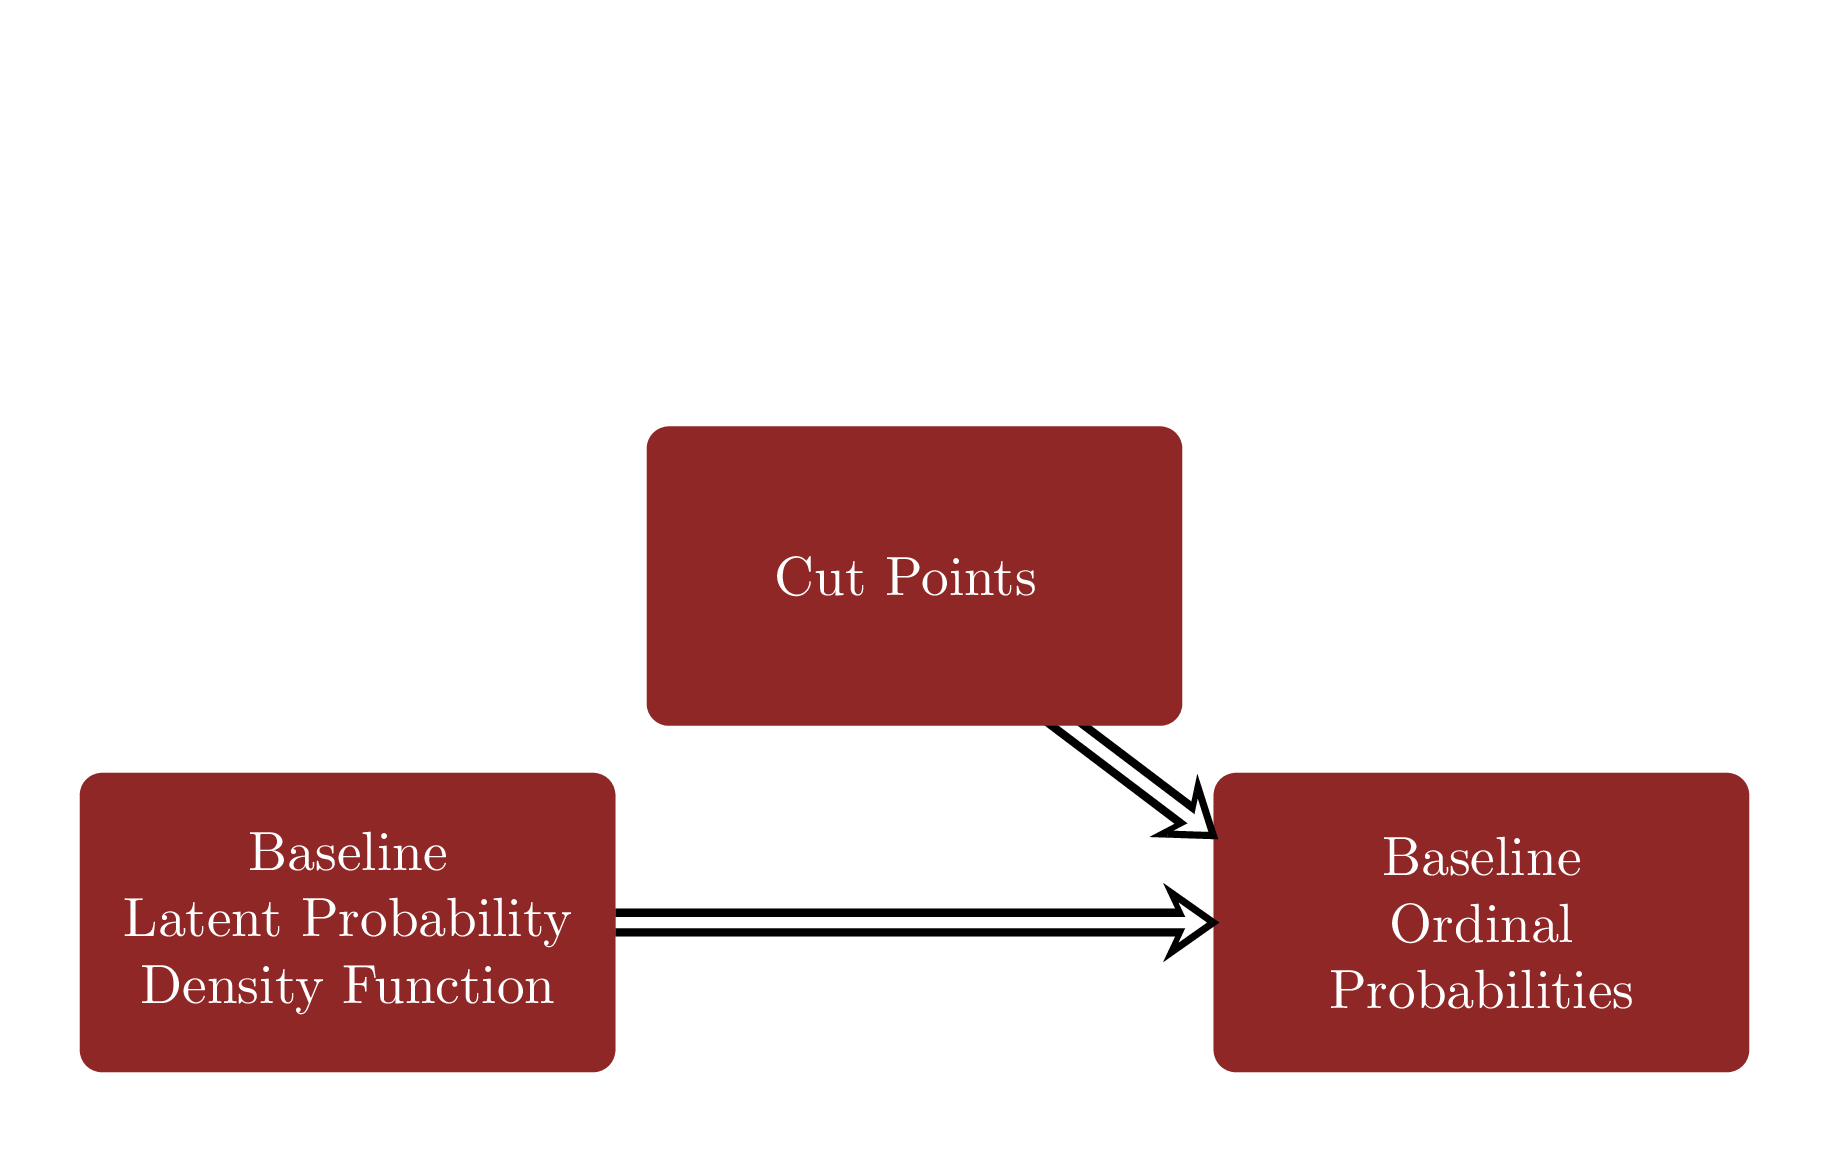
\includegraphics{figures/flow_baseline/flow_baseline.png}

}

\subcaption{\label{fig-flow-baseline}}

\end{minipage}%
%
\begin{minipage}{0.50\linewidth}

\centering{

\captionsetup{labelsep=none}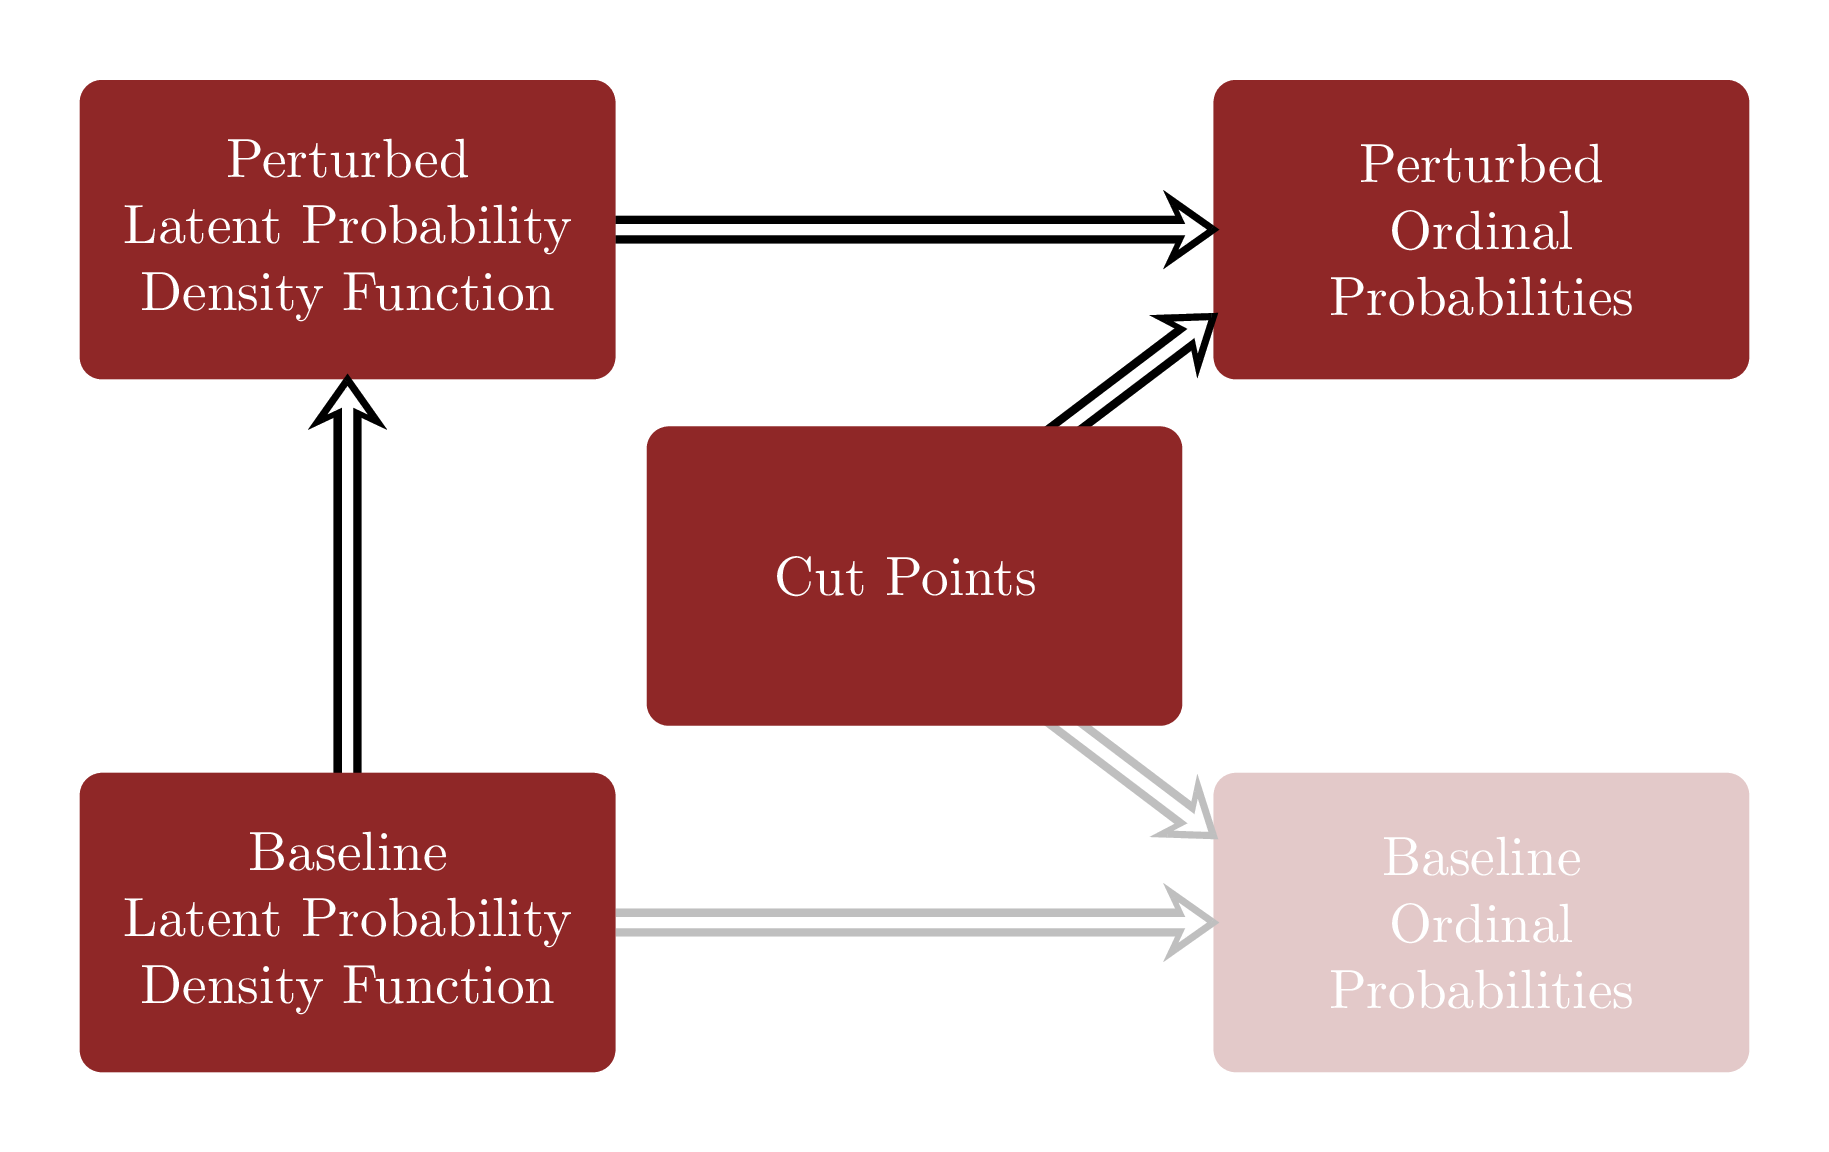
\includegraphics{figures/flow_perturb/flow_perturb.png}

}

\subcaption{\label{fig-flow-perturb}}

\end{minipage}%

\caption{\label{fig-flow}The main utility of the cut point construction
is to model systematic variations in ordinal probabilities. (a) Given a
fixed baseline latent probability density function the cut points will
inform the baseline ordinal probabilities. Consequently any inferences
for the baseline ordinal probabilities will inform consistent cut point
configurations. (b) Once the cut points have been informed we can
perturb the latent probability density function around the baseline
configuration to perturb the ordinal probabilities in a similar way.}

\end{figure}%

In order to increase \(p_{k}\) we have to increase latent probability
density function \(p(x)\) across the interval \((c_{k - 1}, c_{k}]\)
(Figure~\ref{fig-perturb-interval-probs}). The less flexible \(p(x)\) is
the more this will require also increasing \(p(x)\) across the
neighboring intervals, and hence increasing the neighboring ordinal
probabilities \(p_{k - 1}\) and \(p_{k + 1}\). Equivalently if we
engineer \(p(x)\) to decrease \(p_{k}\) then we will likely also
decrease the neighboring probabilities \(p_{k - 1}\) and \(p_{k + 1}\).

\begin{figure}

\centering{

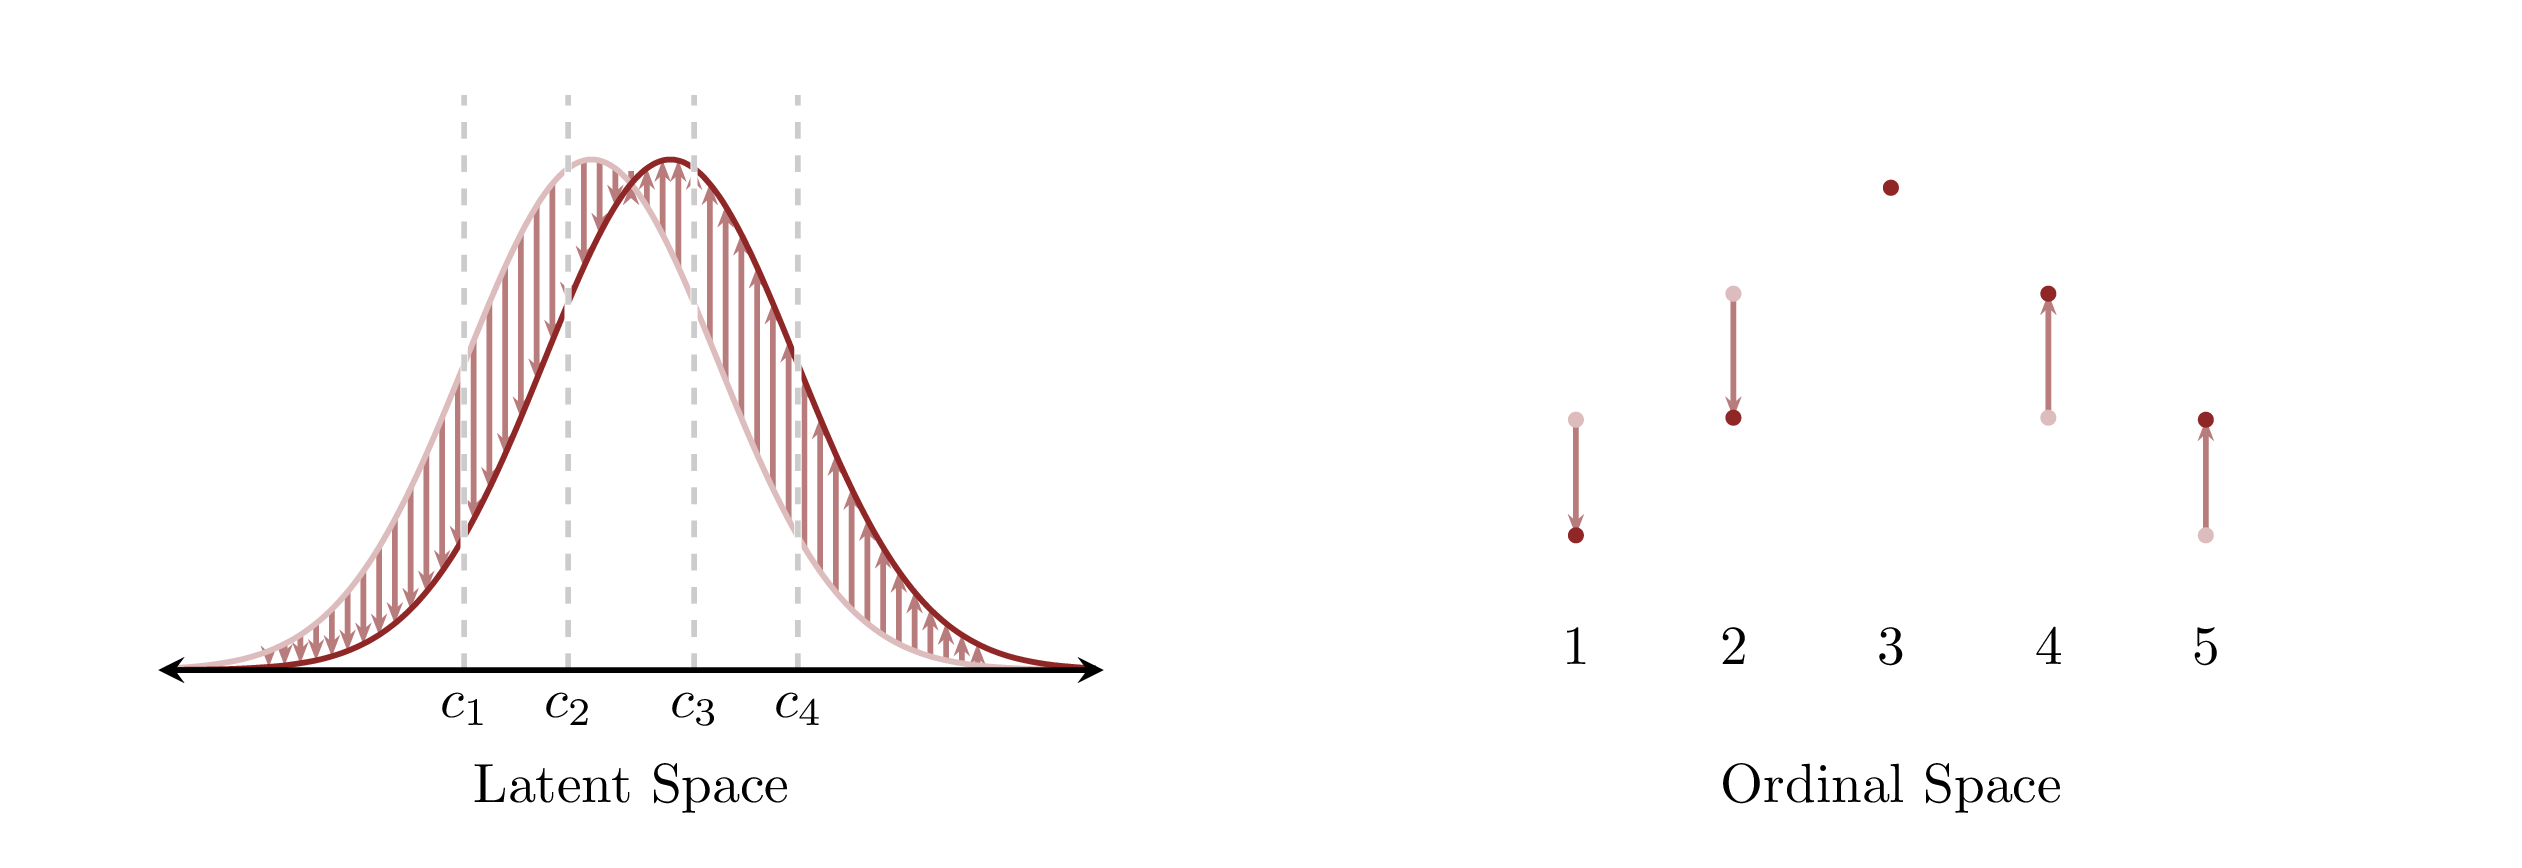
\includegraphics[width=1\textwidth,height=\textheight]{figures/perturb_interval_probs/perturb_interval_probs.png}

}

\caption{\label{fig-perturb-interval-probs}Perturbing the shape of the
latent probability density function perturbs the ordinal probabilities
in a similar way. If the latent probability density function mostly
decreases or increases between two cut points then the corresponding
ordinal probability will decrease or increases as well. The more rigid
the latent probability density function is the more strongly neighboring
ordinal probabilities will be coupled to each other.}

\end{figure}%

For example we might perturb the latent probability distribution by
translating the latent real line to the right, shifting the latent
probability density function towards smaller values. If the interior cut
points are fixed then this pushes the baseline ordinal probabilities
towards smaller ordinal values while preserving the baseline shape.
Likewise translating \(X\) to the left shifts the latent probability
density function towards larger values and pushes the ordinal
probabilities to larger ordinal values
(Figure~\ref{fig-latent-density-translate}). This can be useful when we
want to model how varying conditions might consistently increase or
decrease the sentiment of people answering a survey question.

\begin{figure}

\centering{

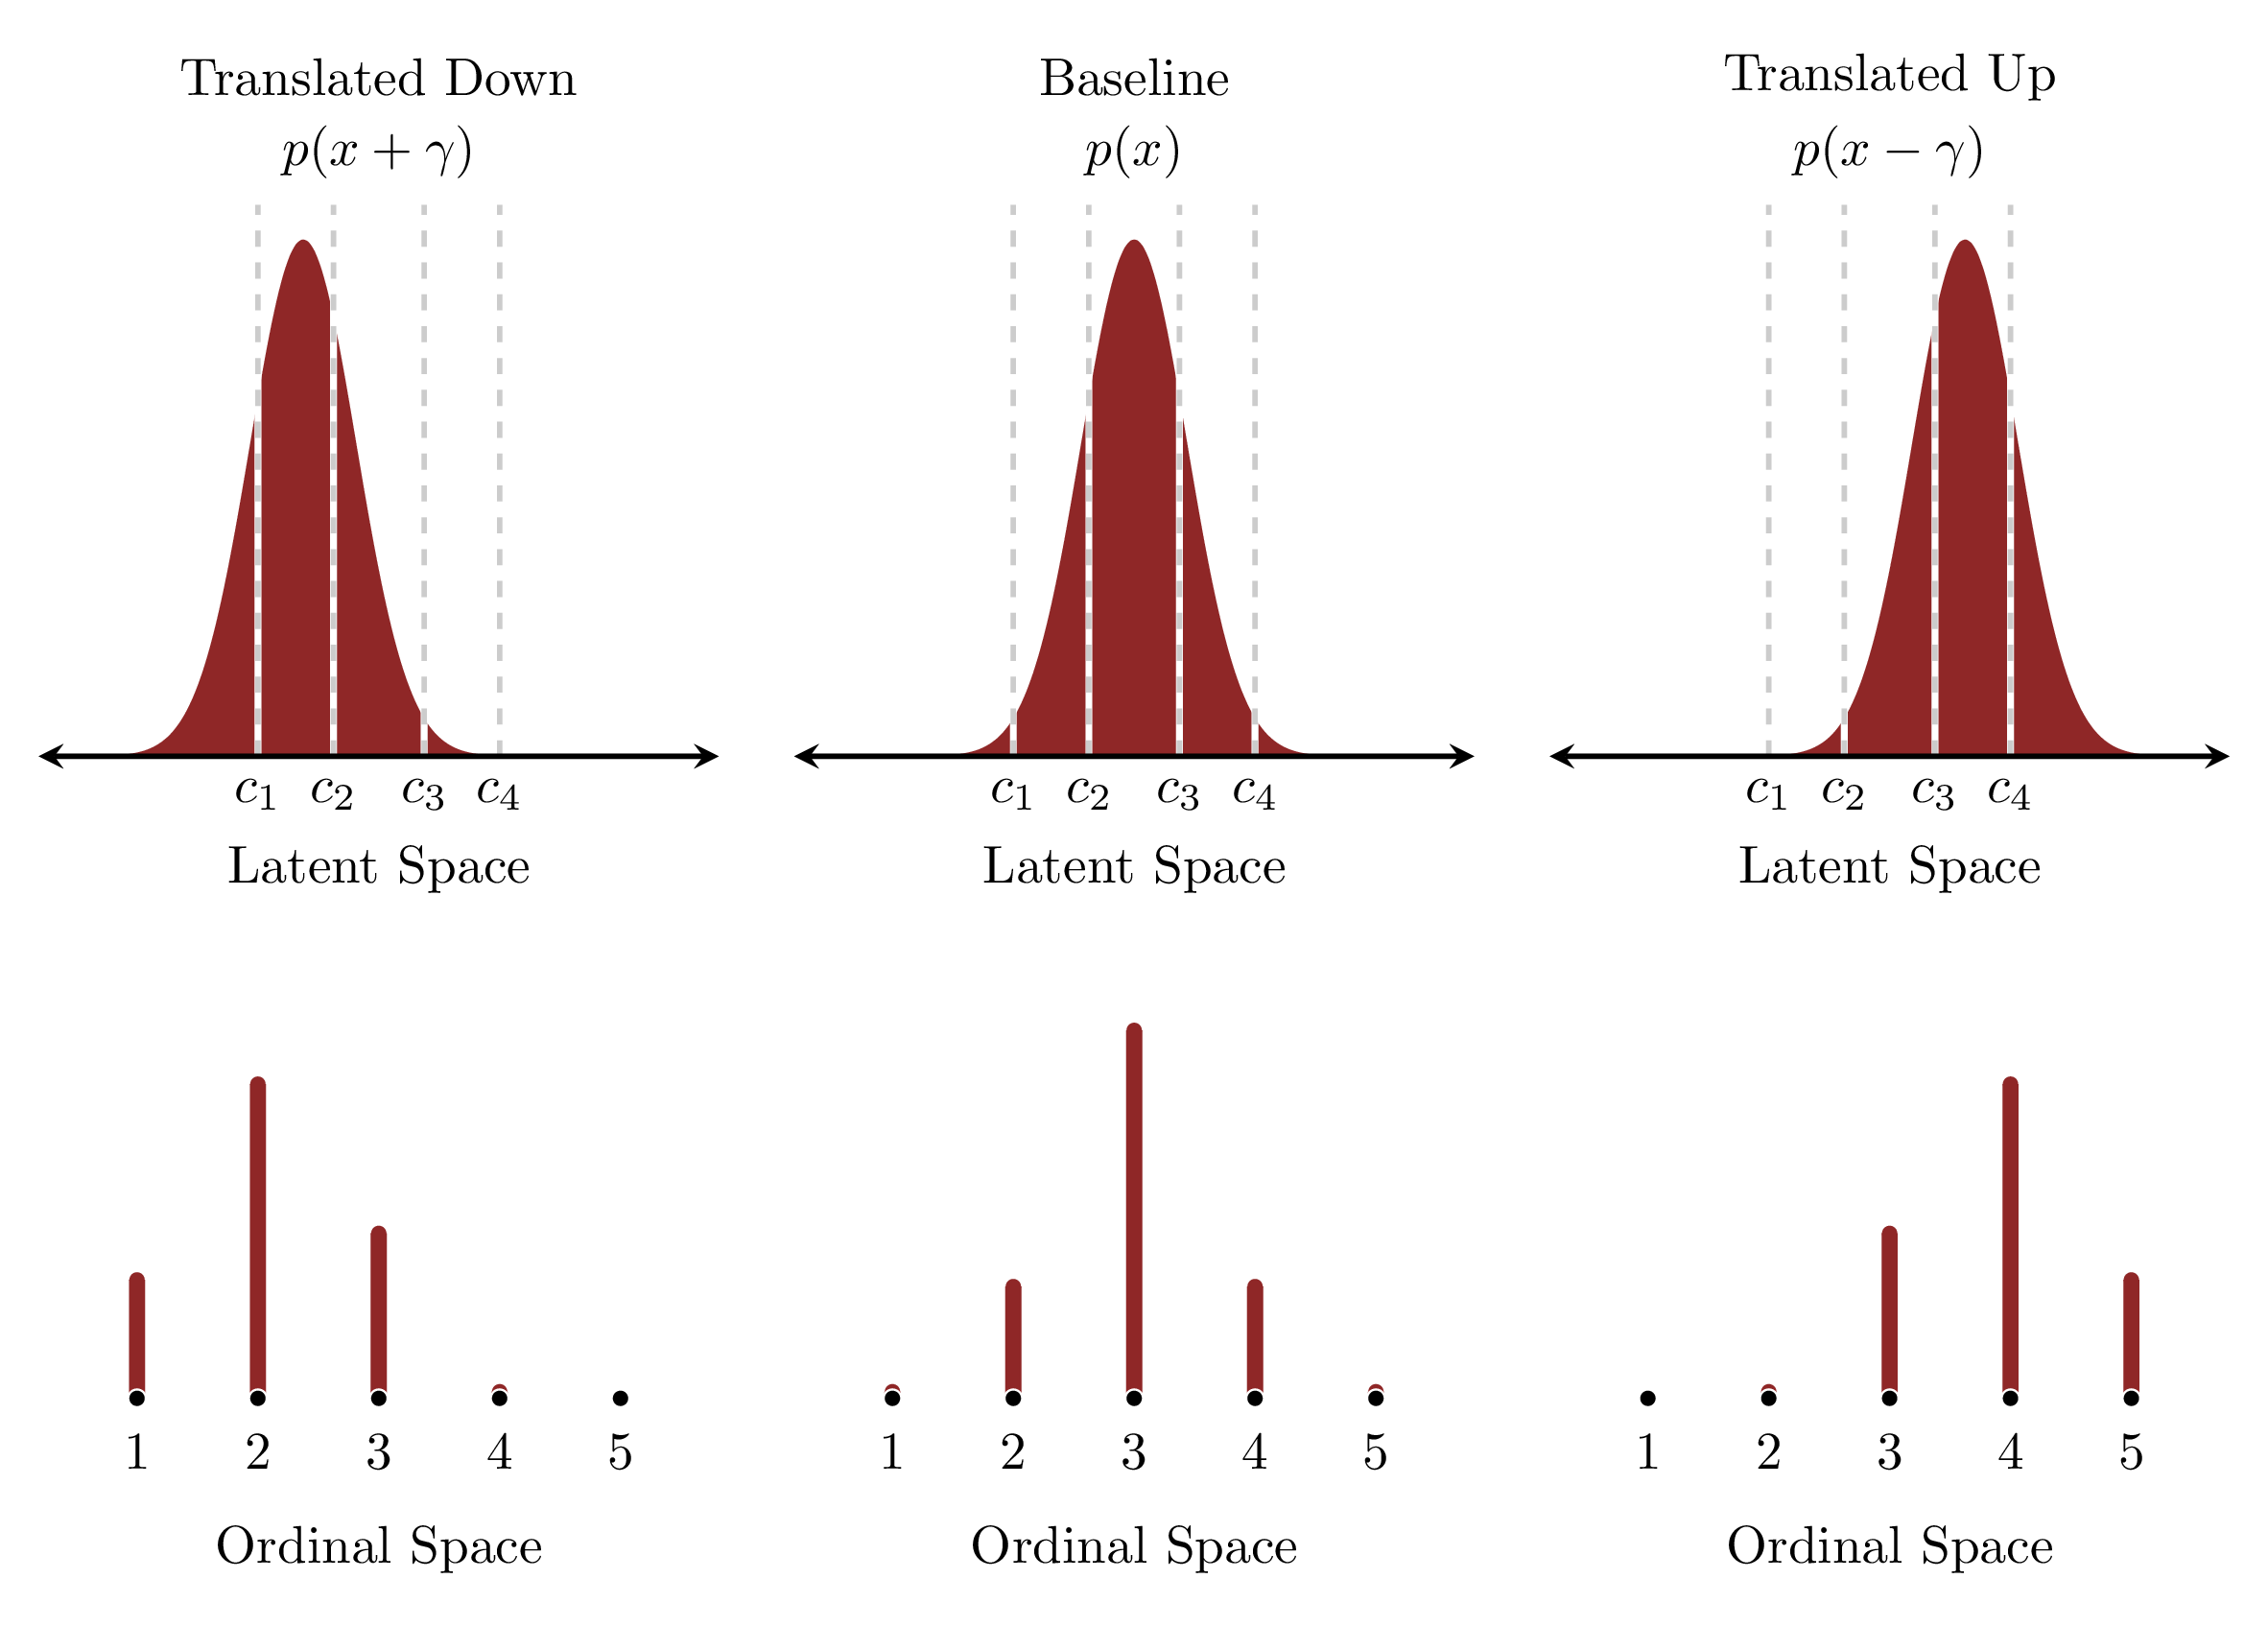
\includegraphics[width=1\textwidth,height=\textheight]{figures/latent_density_translate/latent_density_translate.png}

}

\caption{\label{fig-latent-density-translate}When the cut points are
fixed translating the latent probability density function from its
baseline configuration shifts the ordinal probabilities in the same
direction.}

\end{figure}%

Similarly we might dilate the latent real line, causing the latent
probability density function and the resulting ordinal probabilities to
narrow, or contract the latent real line to widen the latent probability
density function and the resulting ordinal probabilities
(Figure~\ref{fig-latent-density-scale}). This behavior can be useful
when varying conditions might increase or decrease the consistency of
the sentiment of survey responders.

\begin{figure}

\centering{

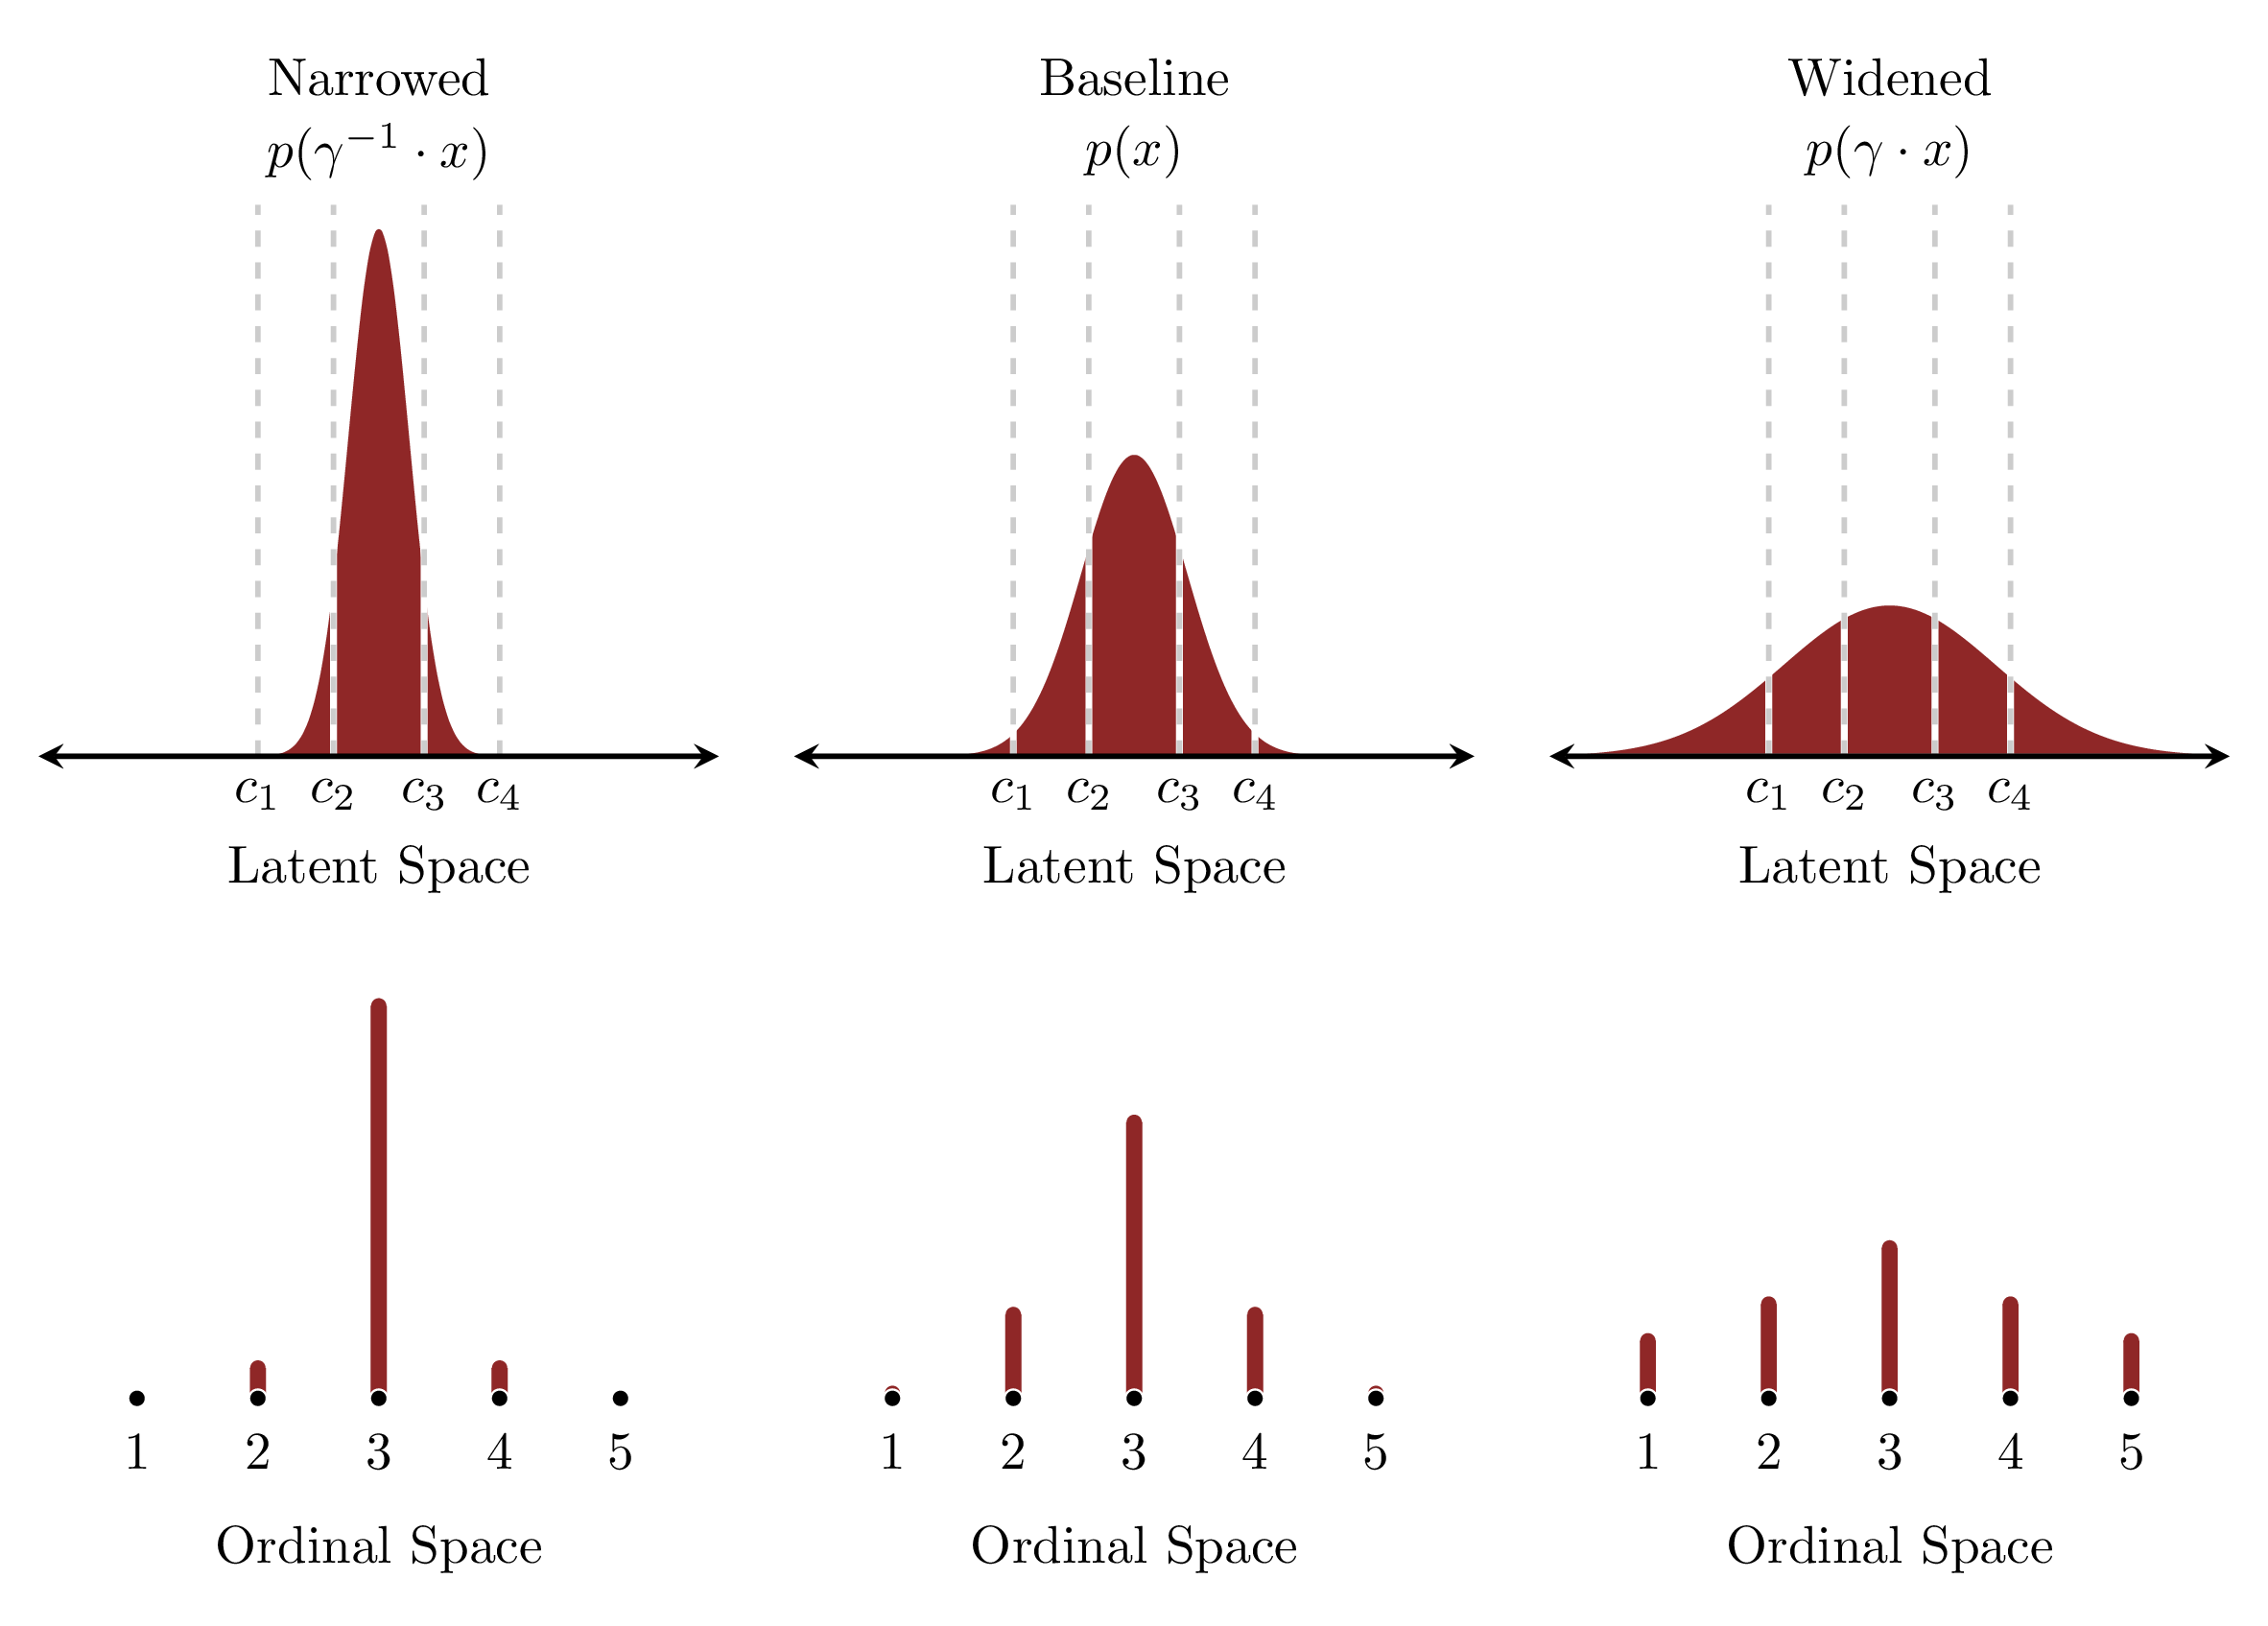
\includegraphics[width=1\textwidth,height=\textheight]{figures/latent_density_scale/latent_density_scale.png}

}

\caption{\label{fig-latent-density-scale}When the cut points are fixed
dilating or contracting the latent probability density function from its
baseline configuration narrows or widens the ordinal probabilities,
respectively.}

\end{figure}%

\subsection{Modeling Heterogeneity with Derived Cut
Points}\label{derived-cuts}

The general strategy for modeling heterogeneous ordinal probabilities is
to

\begin{itemize}
\tightlist
\item
  fix a baseline latent probability density function,
\item
  inform interior cut points from the ordinal probabilities,
\item
  fix the interior cut points,
\item
  vary the ordinal probabilities by varying the configuration of the
  latent probability density function.
\end{itemize}

The most direct way to implement this in practice is to model the
interior cut points and the configuration of the latent probability
density function, deriving the baseline and varying ordinal
probabilities as needed.

That said we can use the duality between interior cut points and ordinal
probabilities to implement this approach another way. Instead of
modeling the interior cut points directly and deriving the baseline
ordinal probabilities, \[
p_{k} = \Pi(c_{k}) - \Pi(c_{k - 1}),
\] we can equivalently model the baseline ordinal probabilities and then
derive the interior cut points, \[
c_{k}
=
\Pi^{-1} \left( \sum_{k' = 1}^{k} p_{k'} \right).
\] Given these derived interior cut points we can then derive varying
ordinal probabilities from varying latent probability density function
configurations as before.

Mathematically these two approaches are equivalent. In practice,
however, the interior cut points and baseline ordinal probabilities
could exhibit different inferential degeneracies that could be more or
less costly depending on the particular observed data and prior model.

Note that in most probabilistic programming tools simplex variables are
handled by first mapping to an unconstrained space with something like
the stick breaking map. Moreover as we saw in
\hyperref[sec:duality]{Section 3.2} the mapping from interior cut points
to ordinal probabilities is very similar to stick breaking. Consequently
any differences in the implementation of these models with either
interior cut points or baseline ordinal probabilities should be small in
practice, although there can always be exceptions.

\subsection{Interpretations of the Cut Point
Construction}\label{interpretations-of-the-cut-point-construction}

In general the cut point construction does not need to model any
particular data generating process. Rather it can be a heuristic
technique to ensure reasonable variations in the ordinal probabilities.
One nice advantage of this perspective is that, because the latent
probability distribution isn't modeling any particular phenomenon, we
can choose the possible latent probability density function
configurations based on implementation convenience or computational
performance.

That said we can use the cut point construction to model an explicit
data generating process when appropriate. For example when ordinal data
arises from the censoring of some unobserved, real-valued behavior then
we can interpret the latent probability distribution as a model of this
behavior with interior cut points modeling how that behavior is censored
in observations.

This narratively generative perspective can be especially useful when
trying to combine inconsistent data into a single analysis. Consider,
for instance, two surveys with the possible responses \[
\text{Disagree}, \text{Neutral}, \text{Agree}
\] and \[
\text{Disagree}, \text{Agree}
\] respectively. Even if the survey responders interpret ``Disagree''
and ``Agree'' consistently between the two surveys it is not obvious to
what responses in the second survey the ``Neutral'' responses in the
first survey would correspond.

If we believe that the survey questions are eliciting some unobserved,
real-valued behavior and we are comfortable modeling that behavior with
a latent probability density function then we can model both surveys
with two sets of cut points to accommodate the inconsistent survey
designs. In this case the set for the first survey would contain two
interior cut points while the set for the second survey would contain a
single interior cut point.

\section{Degeneracies of the Cut Point
Construction}\label{degeneracies-of-the-cut-point-construction}

As with most useful modeling techniques, the cut point construction is
vulnerable to some particular inferential degeneracies that can
frustrate an analysis if we are not prepared to manage them.

\subsection{Latent Non-identifiability}\label{non-ident}

As we saw in \hyperref[derived-probs]{Section 3.1} the cut point
construction defines a map from \(K - 1\) interior cut points into \(K\)
ordinal probabilities given a fixed latent probability density function.
This map is also invertible, allowing us to take \(K\) ordinal
probabilities into \(K - 1\) interior cut points, once again given a
fixed latent probability density function. In other words a latent
probability density function and interior cut points completely specify
ordinal probabilities while a latent probability density function and
ordinal probabilities completely specify interior cut points.

The cut point construction is actually a bit more general than this. Any
configuration of the interior cut points and ordinal probabilities
specify consistent latent probability density functions, although the
specification is not unique in this case. Constraining any \emph{two} of
the three objects in the cut point construction always informs the
third.

If we specify only \emph{one} of these objects, however, then there will
be infinitely many compatible configurations for the other two. Without
care this redundancy can lead to non-identified ordinal models which in
turn result in frustrating inferential degeneracies.

To demonstrate what can go wrong let's say that we do not completely fix
the latent probability density function but instead limit it to a family
of translated probability density functions, \[
p_{\delta}(x) = p_{0}(x + \delta)
\] for some initial probability density function \(p_{0}\). This
translation family then defines the cumulative distribution functions
\begin{align*}
\Pi_{\delta}(x)
&=
\int_{-\infty}^{x} \mathrm{d} x' \, p_{\delta}(x')
\\
&=
\int_{-\infty}^{x} \mathrm{d} x' \, p_{0}(x' + \delta)
\\
&=
\int_{-\infty}^{x + \delta} \mathrm{d} z' \, p_{0} \left( z' \right)
\\
&=
\Pi_{0} ( x + \delta )
\end{align*} and hence the ordinal probabilities \begin{align*}
p_{k}
&=
\Pi_{\delta}(c_{k}) - \Pi_{\delta}(c_{k - 1})
\\
&=
  \Pi_{0} ( c_{k}     + \delta )
- \Pi_{0} ( c_{k - 1} + \delta ).
\end{align*}

Notice, however, that we get the exact same ordinal probabilities if we
set the translation to zero but shift all of the interior cut points by
the same amount, \begin{align*}
p_{k}
&=
  \Pi_{\delta = 0}( c'_{k}     )
- \Pi_{\delta = 0}( c'_{k - 1} )
\\
&=
  \Pi_{\delta = 0}( c_{k}     + \delta )
- \Pi_{\delta = 0}( c_{k - 1} + \delta )
\\
&=
  \Pi_{0} ( c_{k}     + \delta )
- \Pi_{0} ( c_{k - 1} + \delta ).
\end{align*} In other words for each \(\delta\) we have two equivalent
ways of reproducing the same ordinal probabilities.

Similarly translating the latent probability density function and
interior cut points by any amount but in \emph{opposite} directions
always returns the same initial ordinal probabilities
(Figure~\ref{fig-trans-degen}), \begin{align*}
p_{k}
&=
  \Pi_{\delta}(c'_{k}     )
- \Pi_{\delta}(c'_{k - 1} )
\\
&=
  \Pi_{\delta}(c_{k}     - \delta)
- \Pi_{\delta}(c_{k - 1} - \delta)
\\
&=
  \Pi_{0} ( c_{k}     - \delta + \delta )
- \Pi_{0} ( c_{k - 1} - \delta + \delta )
\\
&=
  \Pi_{0} ( c_{k}     )
- \Pi_{0} ( c_{k - 1} ).
\end{align*}

\begin{figure}

\centering{

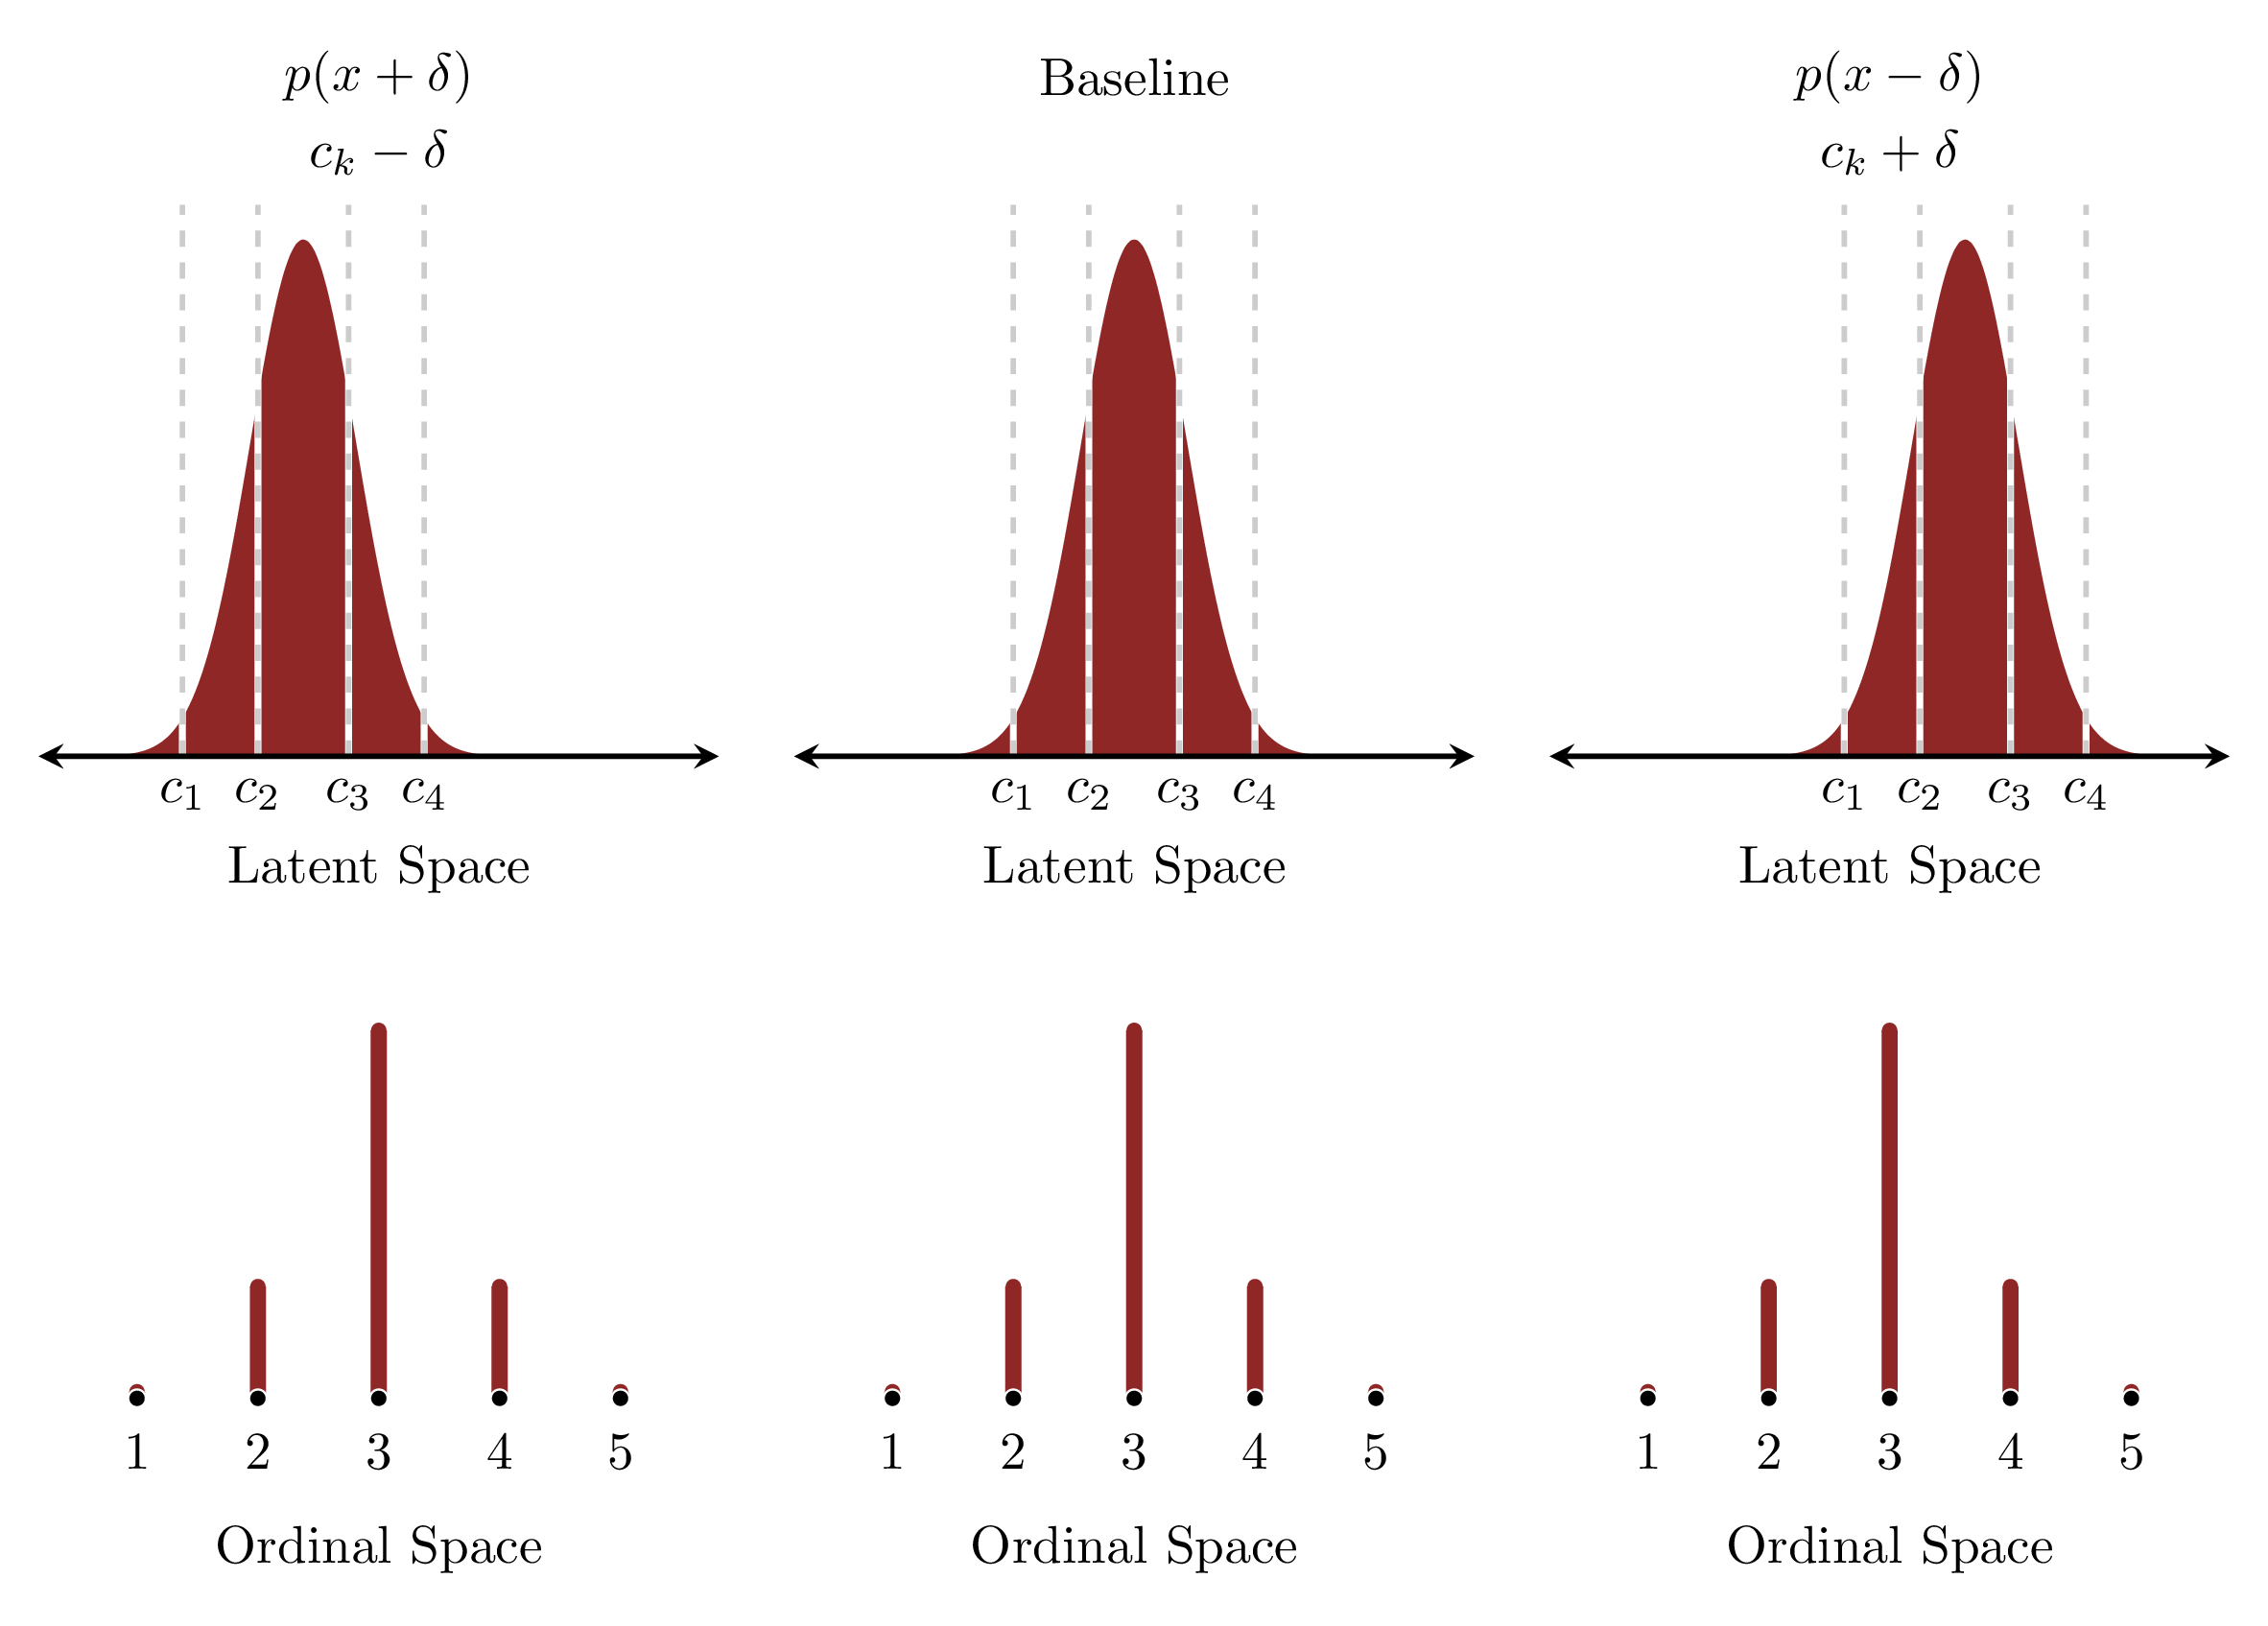
\includegraphics[width=1\textwidth,height=\textheight]{figures/trans_degen/trans_degen.png}

}

\caption{\label{fig-trans-degen}Any change to the latent probability
density function can be compensated by a complementary change to the
interior cut points so that the ordinal probabilities remain the same.
Consequently inferences for the ordinal probabilities cannot inform the
behavior of the latent probability density function and interior cut
points at the same time.}

\end{figure}%

Consequently any constraint on the ordinal probabilities alone, such as
from observed data or domain expertise encoded into a prior model,
cannot disentangle the behavior of the latent probability density
function and the interior cut points \emph{at the same time}.

This degeneracy between the behavior of the latent probability density
function and the interior cut points extends far beyond just
translations, although the math becomes a bit more involved.

Consider a family of latent probability density functions, each element
of which is generated by mapping the latent real line into itself with
an order-preserving function. We can then write each latent probability
density function in the family as \[
p_{f}(x) = p_{0} \left( f^{-1}(x) \right) \,
\left| \frac{ \mathrm{d} f }{ \mathrm{d} x}
       \left( f^{-1}(x) \right) \right|^{-1}
\] for some initial probability density function \(p_{0}\) and any
bijective, monotonically increasing function \[
f : \mathbb{R} \rightarrow \mathbb{R}.
\] The cumulative distribution function for any member of this family is
then given by \begin{align*}
\Pi_{f}(x)
&=
\int_{-\infty}^{x} \mathrm{d} x' \, p_{f}(x')
\\
&=
\int_{-\infty}^{x} \mathrm{d} x' \,
p_{0} \left( f^{-1}(x') \right) \,
\left| \frac{ \mathrm{d} f }{ \mathrm{d} x}
       \left( f^{-1}(x') \right) \right|^{-1}
\\
&=
\int_{-\infty}^{f^{-1}(x)} \mathrm{d} x'' \, p_{0} \left( x'' \right)
\\
&=
\Pi_{0} \left( f^{-1}(x) \right).
\end{align*}

Given a function \(f\) the ordinal probabilities become \begin{align*}
p_{k}
&=
\Pi_{f}(c_{k}) - \Pi_{f}(c_{k - 1})
\\
&=
  \Pi_{0} \left( f^{-1}(c_{k}    ) \right)
- \Pi_{0} \left( f^{-1}(c_{k - 1}) \right).
\end{align*} At the same time if we use the initial probability density
function \(p_{0}\) but transform the interior cuts points using the
inverse of \(f\), \[
c'_{k} = f^{-1}(c_{k}),
\] then the resulting ordinal probabilities are exactly the same as
above, \begin{align*}
p_{k}
&=
  \Pi_{0} \left( c'_{k}     \right)
- \Pi_{0} \left( c'_{k - 1} \right)
\\
&=
  \Pi_{0} \left( f^{-1}(c_{k}    ) \right)
- \Pi_{0} \left( f^{-1}(c_{k - 1}) \right).
\end{align*} For each order-preserving function \(f\) we have two
equivalent ways of reproducing the same ordinal probabilities!

We can also always transform the latent probability density function and
interior cut points in complementary ways to achieve the same initial
ordinal probabilities, \begin{align*}
p_{k}
&=
  \Pi_{f} \left( c'_{k}     \right)
- \Pi_{f} \left( c'_{k - 1} \right)
\\
&=
  \Pi_{f} \left( f(c_{k}     ) \right)
- \Pi_{f} \left( f(c_{k - 1} ) \right)
\\
&=
  \Pi_{0} \left( f^{-1}(f(c_{k}    )) \right)
- \Pi_{0} \left( f^{-1}(f(c_{k - 1})) \right)
\\
&=
  \Pi_{0} ( c_{k}     )
- \Pi_{0} ( c_{k - 1} ).
\end{align*}

In order to avoid these degeneracies we have to constrain, if not
outright fix, any two of the three objects in the cut point construction
at any given time. That said we don't have to constrain the \emph{same}
two objects across an entire analysis. Indeed activating different
objects at different times is what allows us to model heterogeneity in
the ordinal probabilities.

For example when modeling baseline behavior we have to define a fixed
baseline latent probability density function so that any constraints on
the baseline ordinal probabilities will inform the interior cut points.
Because both the latent probability density function and ordinal
probabilities are constrained there are no identifiability concerns.

When modeling behavior outside of the baseline we use these baseline
inferences to constrain the interior cut points. Any constraints on the
heterogeneous ordinal probabilities then inform variations from the
baseline latent probability density function. In this case the interior
cut points and ordinal probabilities are constrained, eliminating any
identifiability concern for the variation of the latent probability
density function.

For a specific example let's say that we want to allow the latent
probability density function to be able to shift in different conditions
so that the resulting ordinal probabilities coherently move towards
smaller and larger ordinal values. We can achieve this with the
translation family that we introduced above, \[
p_{\delta}(x) = p_{0}(x + \delta).
\]

To avoid any identifiability issues we have to fix \(\delta\) to a
particular value when modeling the baseline probabilities. This value is
arbitrary, but often it's convenient to take \(\delta = 0\). Once we
have fixed \(\delta\) we can then use any baseline data and available
domain expertise to inform the consistent behaviors of interior cut
points. Those inferred interior cut point behaviors then allow us to
model observations beyond the baseline context by letting \(\delta\)
vary to accommodate any systematic variations in the ordinal
probabilities.

Altogether we end up with well-behaved joint inferences for the common
interior cut points and a \(\delta_{i}\) for each individual context.

\subsection{Tail Degeneracies}\label{tail-degeneracies}

Even when the latent probability density function is fixed interior cut
points can suffer from another, although much more circumstantial,
degeneracy.

The \(k\)th ordinal probability depends on the \((k - 1)\)st and \(k\)th
cut points. We can quantify the strength of these dependencies with the
corresponding partial derivatives, \begin{align*}
\frac{ \partial p_{k} }{ \partial c_{k} } (c_{1}, \ldots, c_{K})
&=
\frac{ \partial }{ \partial c_{k} }
\left( \Pi( c_{k} ) - \Pi( c_{k - 1} ) \right)
\\
&=
\frac{ \mathrm{d} \Pi }{ \partial x } (c_{k})
\\
&=
p( c_{k} )
\end{align*} and \begin{align*}
\frac{ \partial p_{k} }{ \partial c_{k - 1} } (c_{1}, \ldots, c_{K})
&=
\frac{ \partial }{ \partial c_{k - 1} }
\left( \Pi( c_{k} ) - \Pi( c_{k - 1} ) \right)
\\
&=
- \frac{ \mathrm{d} \Pi }{ \partial x } (c_{k - 1})
\\
&=
-p( c_{k - 1} ).
\end{align*}

In words \(p_{k}\) is least sensitive to changes in \(c_{k - 1}\) when
\(p( c_{k - 1} )\) is small, and it is least sensitive to changes in
\(c_{k}\) when \(p(c_{k})\) is small. An immediate consequence of this
is that if \(p(c_{k})\) is small then any constraints on \(p_{k}\) and
\(p_{k + 1}\) will only poorly inform \(c_{k}\).

When the latent probability density function is unimodal, for example in
the ordered logit and ordered probit models, then \(p(x)\) is smallest
in the tails as \(x\) approaches \(-\infty\) or \(+\infty\).
Unfortunately it's also in the tails that these degeneracies can become
particularly problematic.

Consider, for example, the first ordinal \(k = 1\). If there are no
observations of this particular value then are inferences will be able
to suppress only larger values of the ordinal probability \(p_{1}\),
\begin{align*}
0 &\le \hphantom{\Pi} p_{1} \hphantom{()} \lessapprox \epsilon
\\
0 &\le \Pi(c_{1}) \lessapprox \epsilon.
\end{align*} In theory \(c_{1}\) should also be informed by \(p_{2}\),
but if \(p(c_{1})\) is small then inferences for \(c_{1}\) will be
limited to the consequences of this upper bound, \begin{align*}
0 &\le \Pi(c_{1}) \lessapprox \epsilon
\\
\Pi^{-1}(0) &\le
\hphantom{\Pi(} c_{1} \hphantom{)} \lessapprox
\Pi^{-1}(\epsilon)
\\
-\infty &<
\hphantom{\Pi(} c_{1} \hphantom{)}
\lessapprox \Pi^{-1}(\epsilon).
\end{align*}

In this case arbitrary negative values of \(c_{1}\) will be consistent
with the observed data, with the likelihood function remaining non-zero
even as \(c_{1}\) approaches minus infinity
(Figure~\ref{fig-tail-degen}). Without any compensating prior
information this degeneracy will then manifest in the posterior
distribution, tempting Markov chains into burning endless computation in
an attempt to chase that infinity.

\begin{figure}

\centering{

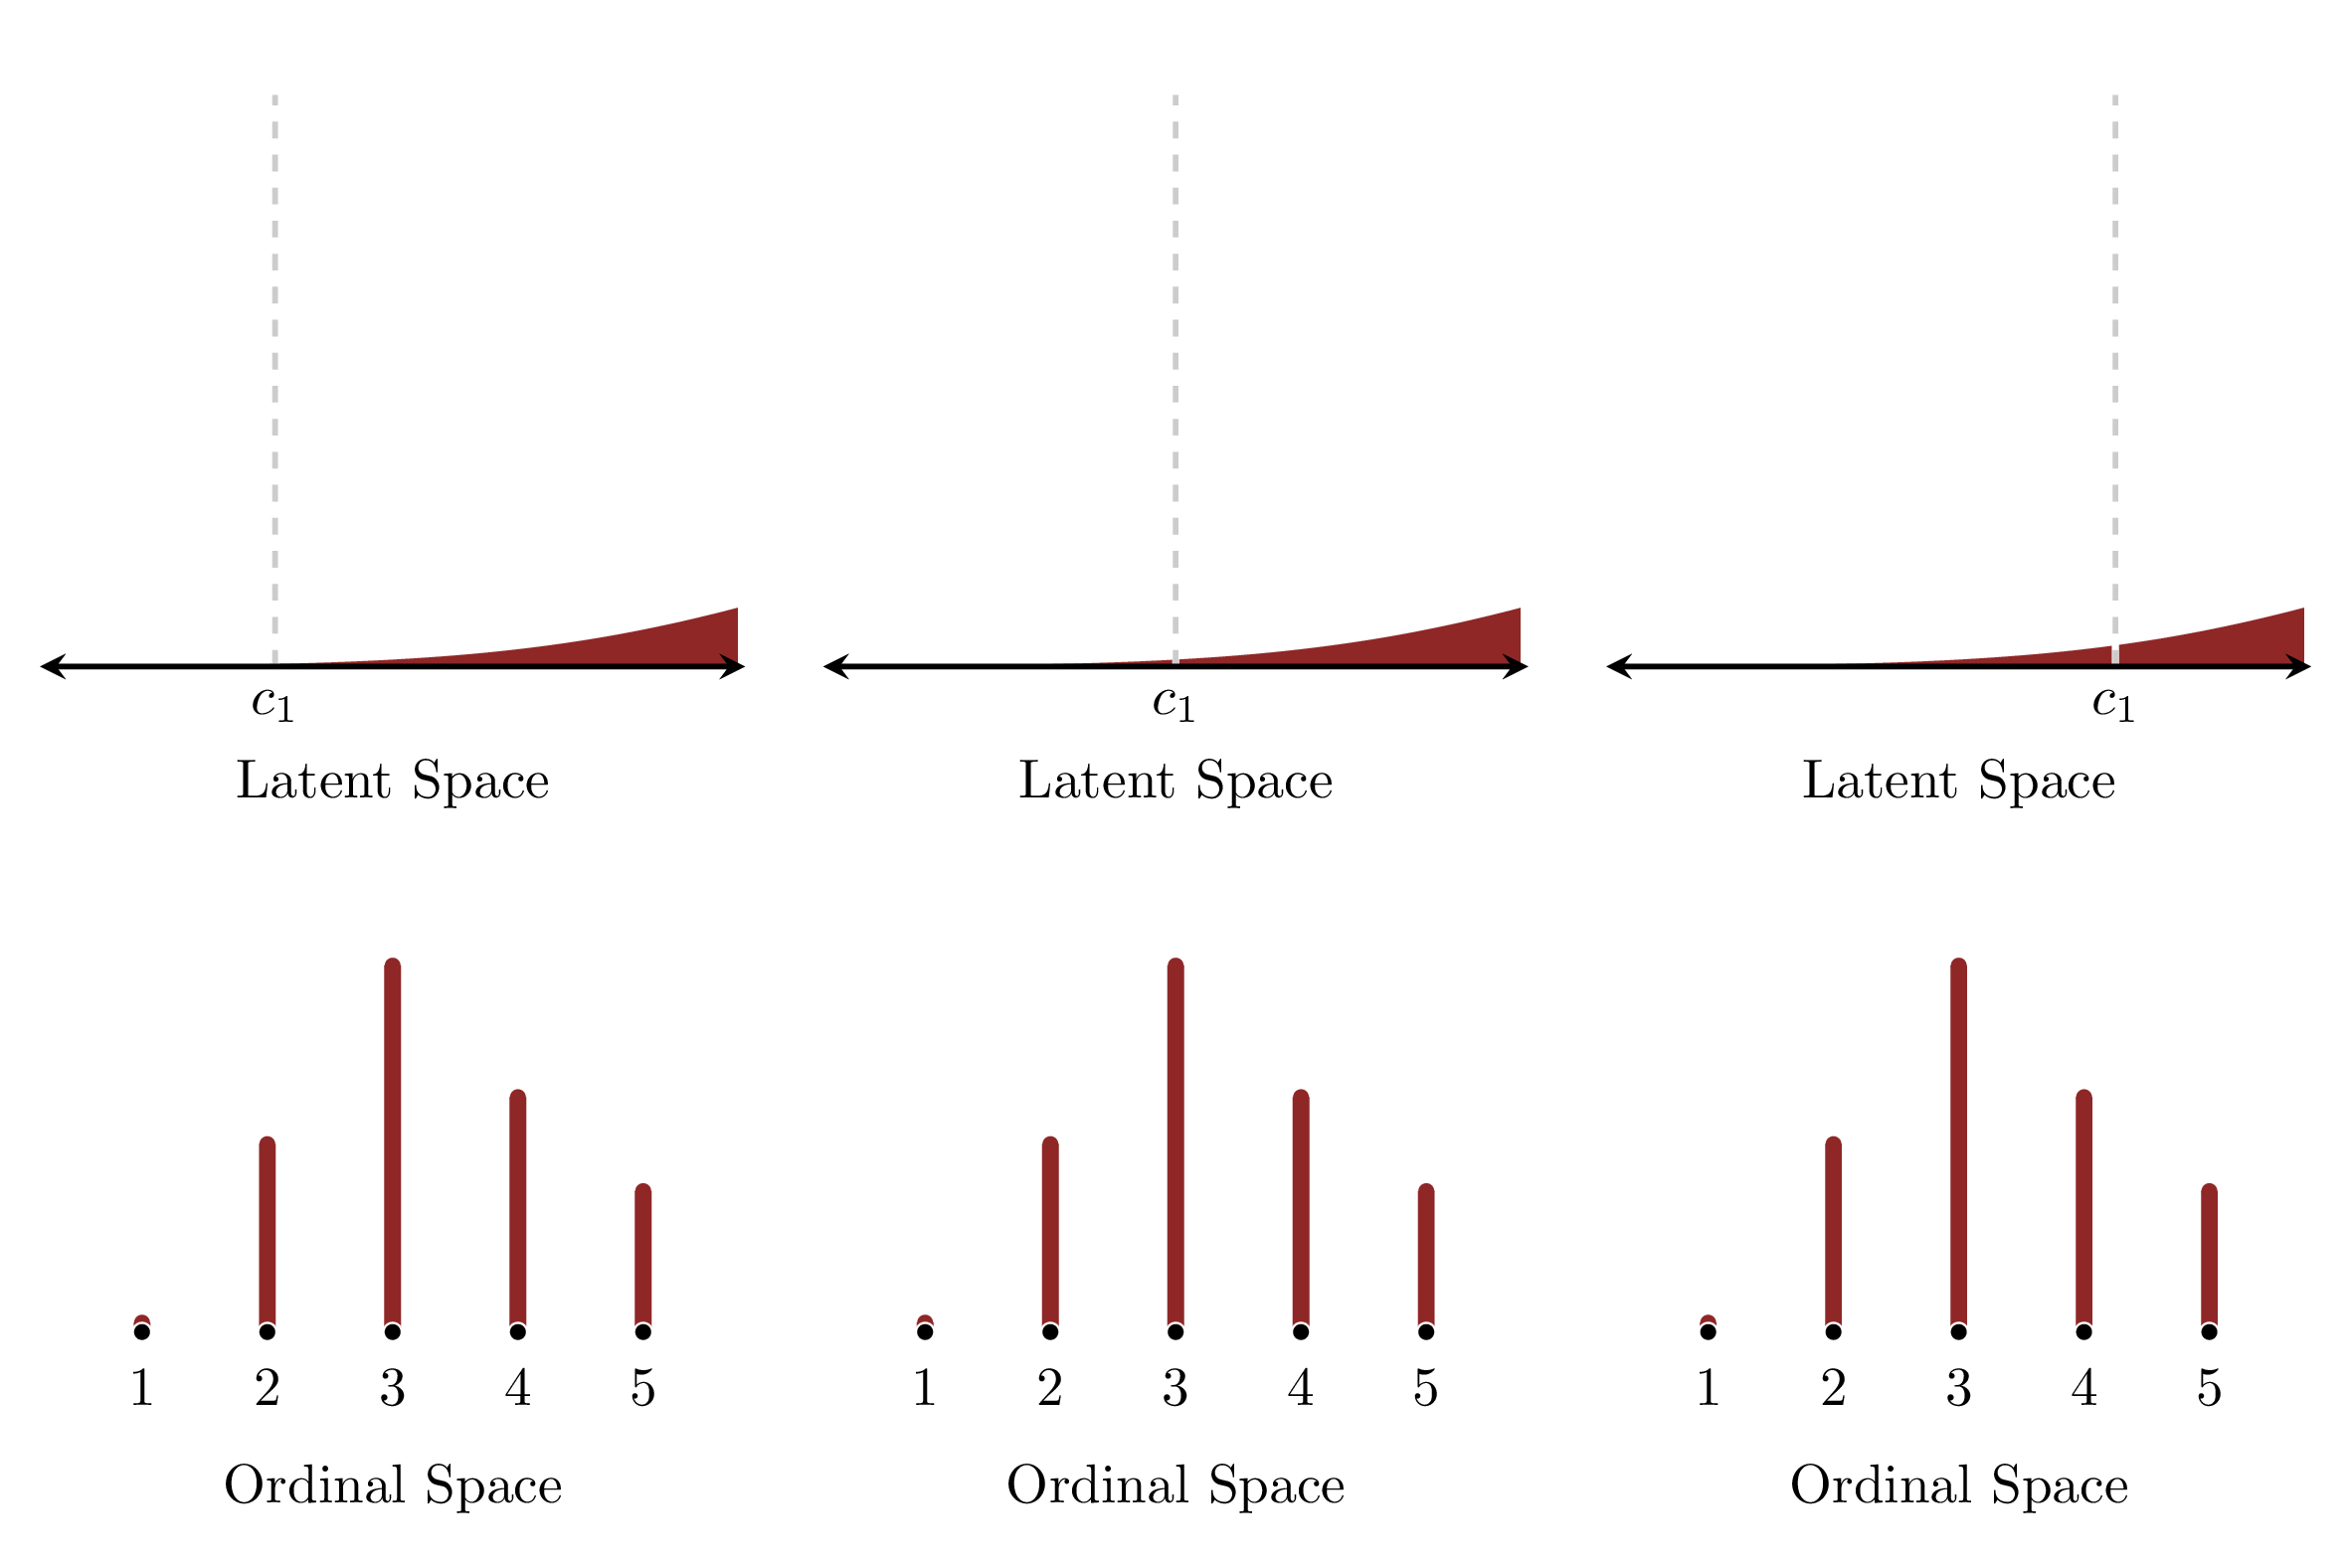
\includegraphics[width=1\textwidth,height=\textheight]{figures/tail_degen/tail_degen.png}

}

\caption{\label{fig-tail-degen}When the first ordinal probability
\(p_{1}\) is close to zero the first interior cut point \(p_{1}\) will
typically fall into the tail of the latent probability density function.
Here even large changes to \(c_{1}\) will have only a negligible impact
on \(p_{1}\) and the neighboring \(p_{2}\). In this case arbitrarily
small values of \(c_{1}\) will be consistent with most observations no
matter the behavior of \(p_{2}\).}

\end{figure}%

A similar problem can arise for the last ordinal. If we don't have any
observations for \(k = K\) then the observed data will be able to only
upper bound \(p_{K}\), \[
0 \le p_{K} \lessapprox \epsilon.
\] If \(p(c_{K - 1})\) is small then the best constraint on
\(c_{K - 1}\) will be an approximate lower bound, \begin{align*}
0 &\le \hphantom{1 - \Pi} p_{K} \hphantom{(_{-1})} \lessapprox \epsilon
\\
0 &\le 1 - \Pi(c_{K - 1}) \lessapprox \epsilon
\\
1 - \epsilon &\lessapprox \Pi(c_{K - 1}) \le 1
\\
\Pi^{-1}(1 - \epsilon) &\lessapprox
\hphantom{\Pi(} c_{K - 1} \hphantom{)} \le
\Pi^{-1}(1)
\\
\Pi^{-1}(1 - \epsilon) &\lessapprox
\hphantom{\Pi(} c_{K - 1} \hphantom{)} <
+\infty,
\end{align*} resulting in a likelihood function that persists all the
way to positive infinity.

The best way to safeguard against either of these tail degeneracies is
to complement the ordinal model with an informative prior model that
suppresses cut point configurations near infinity. Coincidentally we'll
discuss a convenient method for this in the next section.

\section{Informing Cut Points with Domain
Expertise}\label{informing-cut-points-with-domain-expertise}

Because interior cut points are defined only relative to a latent
probability density function they are not the most interpretable
objects. This lack of interpretability can limit our ability to elicit
useful domain expertise which then frustrates any attempt at principled
prior modeling.

Ordinal probabilities, however, enjoy a much more direct interpretation
that facilitates prior modeling. For example we might engineer a
Dirichlet prior \[
p( p_{1}, \ldots, p_{K} )
=
\text{Dirichlet}( p_{1}, \ldots, p_{K} \mid
                  \alpha_{1}, \ldots, \alpha_{K})
\] compatible with our domain expertise.

Taking \[
\alpha_{1} = \ldots = \alpha_{k} = \ldots = \alpha_{K} = 1
\] yields a uniform prior density function over all possible ordinal
probabilities. On the other hand taking \[
\alpha_{k} = \rho_{k} / \tau + 1
\] gives a prior model that concentrates around the ordinal
probabilities \((\rho_{1}, \ldots, \rho_{K})\) with \(\tau\) controlling
the strength of that concentration.

Now given a fixed latent probability density function the ordinal
probabilities completely determine the interior cut points and vice
versa. Consequently once the latent probability density function is
fixed we can to translate any prior model over the ordinal probabilities
into an \emph{induced} prior model over the interior cut points. More
formally we can push the prior model forward from the simplex of ordinal
probabilities to the space of interior cut points.

Consider a fixed latent probability density function \(p\) and
cumulative distribution function \[
\Pi(x) = \int_{-\infty}^{x} \mathrm{d} x' \, p(x').
\] Given the ordinal probabilities \[
\mathbf{p} = (p_{1}, \ldots, p_{K})
\] the interior cut points \[
\mathbf{c} = (c_{1}, \ldots, c_{K - 1})
\] are given by the components \[
c_{k}
=
\left( \phi( \mathbf{p} ) \right)_{k}
=
\Pi^{-1} \left( \sum_{k' = 1}^{k} p_{k'} \right)
\] with the inverse components \[
p_{k}
=
\left( \phi^{-1}( \mathbf{c} ) \right)_{k}
=
\Pi(c_{k}) - \Pi(c_{k - 1}).
\]

Any probability density function over the ordinal probabilities
\(p(\mathbf{p})\) then pushes forward to an equivalent probability
density function over the interior cut points \[
p( \mathbf{c} )
=
p \left( \mathbf{p} = \phi^{-1}(\mathbf{c}) \right)
\cdot \left| \det \mathbf{J}_{\phi^{-1}} (\mathbf{c}) \right|.
\]

The elements of the Jacobian matrix
\(\mathbf{J}_{\phi^{-1}}(\mathbf{c})\) are defined by the partial
derivatives \[
J_{k,k'} (\mathbf{c})
=
\frac{ \partial \phi^{-1}_{k} }{ \partial c_{k'} } (\mathbf{c}).
\] Because each \(p_{k}\) depends on only two neighboring cut points
this results in a banded, upper-diagonal matrix. On the diagonal we have
\[
J_{k,k} (\mathbf{c})
=
\frac{ \partial \phi^{-1}_{k} }{ \partial c_{k} } (\mathbf{c})
=
\frac{ \mathrm{d} \Pi }{ \mathrm{d} x }(c_{k})
=
p(c_{k}).
\] Similarly just above the diagonal we have \[
J_{k,k + 1} (\mathbf{c} )
=
\frac{ \partial f^{-1}_{k} }{ \partial c_{k + 1} } (\mathbf{c})
=
-\frac{ \mathrm{d} \Pi }{ \mathrm{d} x }(c_{k + 1})
=
-p(c_{k}),
\]

For example if \(K = 5\) then the Jacobian matrix would be the four by
four matrix \[
\mathbf{J}_{\phi^{-1}} ( \mathbf{c} )
=
\begin{pmatrix}
 p(c_{1}) &
-p(c_{2}) &
        0 &
        0 \\
        0 &
\hphantom{-} p(c_{2}) &
-p(c_{3}) &
        0 \\
        0 &
        0 &
\hphantom{-} p(c_{3}) &
-p(c_{4}) \\
        0 &
        0 &
        0 &
\hphantom{-} p(c_{4})
\end{pmatrix}.
\]

Conveniently the determinant of an upper-diagonal matrix is just the
product of its diagonal elements, \[
\det \mathbf{J}_{\phi^{-1}} ( \mathbf{c} )
=
\prod_{k = 1}^{K - 1} p(c_{k}).
\] When implementing a log probability density function this simplifies
even further to \[
\log | \det \mathbf{J} \left( \phi^{-1}(\mathbf{c}) \right) |
=
\sum_{k = 1}^{K - 1}
\log p(c_{k}).
\]

If our domain expertise is consistent with the Dirichlet prior model \[
\text{Dirichlet} \left( \mathbf{p} \mid
                        \alpha_{1}, \ldots, \alpha_{K} \right)
\] then the equivalent prior model over the interior cut points is given
by \[
p( \mathbf{c} )
\text{Dirichlet} \left( \phi^{-1}(\mathbf{c}) \mid
                  \alpha_{1}, \ldots, \alpha_{K} \right)
\cdot \left| \prod_{k = 1}^{K - 1} p(c_{k}) \right|.
\] I will refer to this as the \textbf{induced Dirichlet model}.

Keep in mind that any induced prior model over the interior cut points
is defined relative to an appropriate latent probability density
function. If that latent probability density function is not consistent
with the rest of the model then the induced prior model will not capture
the desired domain expertise. For instance if we're modeling
heterogeneous ordinal probabilities and we have domain expertise about
the baseline ordinal probabilities then we have to use the baseline
latent probability density function to define the induced prior model.

Lastly if, as discussed in \hyperref[derived-cuts]{Section 3.4}, we're
parameterizing the ordinal model in terms of baseline ordinal
probabilities and then deriving the interior cut points then we can just
directly use any prior model for those ordinal probabilities.

\section{Ordinal Pairwise Comparison
Modeling}\label{ordinal-pairwise-comparison-modeling}

One common application of the cut point construction is modeling
bipartide
\href{https://betanalpha.github.io/assets/chapters_html/pairwise_comparison_modeling.html}{pairwise
comparisons} with ordinal outputs. That said this particular application
introduces a few subtleties that warrant some careful consideration.

\subsection{Homogeneous Cut Points}\label{homogeneous-cut-points}

In these applications we are usually interested in quantifying how
individual \textbf{appraiser} items express ordinal sentiments about
\textbf{appraisee} items. The quality of an appraisee, \(\gamma_{j}\),
quantifies its general appeal while the quality of an appraiser,
\(\alpha_{i}\), determines how austere their responses tend to be.

We can then use the difference in these item qualities to translate a
latent probability function relative to fixed cut points, \[
p_{ij}(x) = p_{0}(x - (\gamma_{j} - \alpha_{i}) ),
\] resulting in the varying ordinal probabilities \[
p_{k} =
  \Pi_{0}( c_{k}     - (\gamma_{j} - \alpha_{i}) )
- \Pi_{0}( c_{k - 1} - (\gamma_{j} - \alpha_{i}) ).
\] The configuration of the cut points determines the shape of the
baseline ordinal probabilities which models how the appraisers translate
their complex sentiments into the available ordinal values.

When the \(i\)th appraiser's austerity is larger than the \(j\)th
appraisee's appeal then \[
\alpha_{i} > \gamma_{j}
\] and \[
\gamma_{j} - \alpha_{i} < 0.
\] In this case the latent probability density function, and the
resulting ordinal probabilities, shift towards smaller ordinal values,
consistent with a more negative response.

Conversely if the appraisee's appeal is larger than the appraiser's
austerity then \[
\gamma_{j} > \alpha_{i}
\] and \[
\gamma_{j} - \alpha_{i} > 0.
\] This causes the ordinal probabilities to shift towards larger ordinal
values, consistent with a more positive response.

Now as we saw in \hyperref[non-ident]{Section 4.1} we need to bind the
interior cut points to a specific baseline latent probability density
function in order to avoid inferential degeneracies. In this pairwise
comparison setting the natural baseline is \(p_{0}(x)\) which
corresponds to a comparison between two equally matched items, \[
\gamma_{j_{b}} - \alpha_{i_{b}} = 0,
\] or \[
\alpha_{i_{b}} = \gamma_{j_{b}}.
\] Note that the items \(i_{b}\) and \(j_{b}\) do not have to correspond
to any observed items. This baseline comparison can be, and in practice
often is, completely hypothetical.

We're not quite out of the woods yet. To avoid a degeneracy between the
two types of item qualities we also need to anchor at least one item
quality to zero. For instance we might anchor the baseline appraiser
austerity to zero, \[
\gamma_{j_{b}} = 0.
\] In tandem with the previous constraint this would also imply \[
\alpha_{i_{b}} = 0.
\]

\subsection{Heterogeneous Cut Points}\label{heterogeneous-cut-points}

All of this said, in many applications the translation of implicit,
qualitative sentiment into explicit, quantitative ordinal value is not
universal but rather idiosyncratic to each appraiser. Some appraisers
might be more generous with their responses than others, while some
might exhibit more variability in their responses than others.

If we want to model these heterogeneous baseline behaviors then we need
to use a separate set of interior cut points for \emph{each} appraiser,
\(\mathbf{c}_{i}\). This, however, results in comparisons that always
consider the same appraiser austerity \(\alpha_{i}\) and the same set of
interior cut points \(\mathbf{c}_{i}\), with only the appraisee appeals
\(\gamma_{j}\) varying across comparisons.

This means that to avoid inferential degeneracies we have to set
\(\alpha_{i}\) to zero for \emph{every} appraiser. The latent
probability density function configurations for each comparison are then
given by \[
p_{ij}(x) = p_{0}( x - \gamma_{j} ),
\] with the corresponding the ordinal probabilities \[
p_{i, k} =
  \Pi_{0}( c_{i, k}     - \gamma_{j} )
- \Pi_{0}( c_{i, k - 1} - \gamma_{j} ).
\] Intuitively the appraiser austerities have been effectively
``absorbed'' into the appraiser interior cut points.

Many introductions to ordinal modeling start with this final result,
obscuring the underlying pairwise comparison model and the baseline
assumptions we have made along the way. For example without an
understanding of this derivation it may not be obvious that the
appraisee appeals \(\gamma_{j}\) have no absolute meaning on their own,
but rather can be interpreted only relative to each other.

\section{Demonstrations}\label{demonstrations}

Now let's put all of this theory into practice with a series of
demonstrative examples.

\subsection{Set up}\label{set-up}

First we need to setup the local \texttt{R} environment.

\begin{Shaded}
\begin{Highlighting}[]
\FunctionTok{par}\NormalTok{(}\AttributeTok{family=}\StringTok{"serif"}\NormalTok{, }\AttributeTok{las=}\DecValTok{1}\NormalTok{, }\AttributeTok{bty=}\StringTok{"l"}\NormalTok{,}
    \AttributeTok{cex.axis=}\DecValTok{1}\NormalTok{, }\AttributeTok{cex.lab=}\DecValTok{1}\NormalTok{, }\AttributeTok{cex.main=}\DecValTok{1}\NormalTok{,}
    \AttributeTok{xaxs=}\StringTok{"i"}\NormalTok{, }\AttributeTok{yaxs=}\StringTok{"i"}\NormalTok{, }\AttributeTok{mar =} \FunctionTok{c}\NormalTok{(}\DecValTok{5}\NormalTok{, }\DecValTok{5}\NormalTok{, }\DecValTok{3}\NormalTok{, }\DecValTok{5}\NormalTok{))}
\end{Highlighting}
\end{Shaded}

\begin{Shaded}
\begin{Highlighting}[]
\FunctionTok{library}\NormalTok{(rstan)}
\FunctionTok{rstan\_options}\NormalTok{(}\AttributeTok{auto\_write =} \ConstantTok{TRUE}\NormalTok{)            }\CommentTok{\# Cache compiled Stan programs}
\FunctionTok{options}\NormalTok{(}\AttributeTok{mc.cores =}\NormalTok{ parallel}\SpecialCharTok{::}\FunctionTok{detectCores}\NormalTok{()) }\CommentTok{\# Parallelize chains}
\NormalTok{parallel}\SpecialCharTok{:::}\FunctionTok{setDefaultClusterOptions}\NormalTok{(}\AttributeTok{setup\_strategy =} \StringTok{"sequential"}\NormalTok{)}
\end{Highlighting}
\end{Shaded}

\begin{Shaded}
\begin{Highlighting}[]
\NormalTok{util }\OtherTok{\textless{}{-}} \FunctionTok{new.env}\NormalTok{()}
\FunctionTok{source}\NormalTok{(}\StringTok{\textquotesingle{}mcmc\_analysis\_tools\_rstan.R\textquotesingle{}}\NormalTok{, }\AttributeTok{local=}\NormalTok{util)}
\FunctionTok{source}\NormalTok{(}\StringTok{\textquotesingle{}mcmc\_visualization\_tools.R\textquotesingle{}}\NormalTok{, }\AttributeTok{local=}\NormalTok{util)}
\end{Highlighting}
\end{Shaded}

\subsection{Homogeneous Ordinal Probabilities
I}\label{homogeneous-ordinal-probabilities-i}

Let's start by modeling a single set of ordinal probabilities.

\subsubsection{Data Exploration}\label{data-exploration}

Our first data set consists of 50 observations, each of which can take
one of five ordinal values.

\begin{Shaded}
\begin{Highlighting}[]
\NormalTok{data }\OtherTok{\textless{}{-}} \FunctionTok{read\_rdump}\NormalTok{(}\StringTok{\textquotesingle{}data/1.data.R\textquotesingle{}}\NormalTok{)}
\end{Highlighting}
\end{Shaded}

\begin{Shaded}
\begin{Highlighting}[]
\FunctionTok{cat}\NormalTok{(}\FunctionTok{sprintf}\NormalTok{(}\StringTok{\textquotesingle{}\%i ordinal values\textquotesingle{}}\NormalTok{, data}\SpecialCharTok{$}\NormalTok{K))}
\end{Highlighting}
\end{Shaded}

\begin{verbatim}
5 ordinal values
\end{verbatim}

\begin{Shaded}
\begin{Highlighting}[]
\FunctionTok{cat}\NormalTok{(}\FunctionTok{sprintf}\NormalTok{(}\StringTok{\textquotesingle{}\%i total observations\textquotesingle{}}\NormalTok{, data}\SpecialCharTok{$}\NormalTok{N))}
\end{Highlighting}
\end{Shaded}

\begin{verbatim}
50 total observations
\end{verbatim}

The ordinal data are neatly summarized with a histogram.

\begin{Shaded}
\begin{Highlighting}[]
\FunctionTok{par}\NormalTok{(}\AttributeTok{mfrow=}\FunctionTok{c}\NormalTok{(}\DecValTok{1}\NormalTok{, }\DecValTok{1}\NormalTok{), }\AttributeTok{mar=}\FunctionTok{c}\NormalTok{(}\DecValTok{5}\NormalTok{, }\DecValTok{5}\NormalTok{, }\DecValTok{1}\NormalTok{, }\DecValTok{1}\NormalTok{))}

\NormalTok{util}\SpecialCharTok{$}\FunctionTok{plot\_line\_hist}\NormalTok{(data}\SpecialCharTok{$}\NormalTok{y, }\FloatTok{0.5}\NormalTok{, }\FloatTok{5.5}\NormalTok{, }\DecValTok{1}\NormalTok{,}
                    \AttributeTok{xlab=}\StringTok{"Ordinal"}\NormalTok{)}
\end{Highlighting}
\end{Shaded}

\includegraphics{ordinal_modeling_files/figure-pdf/unnamed-chunk-7-1.pdf}

\subsubsection{Categorical Model}\label{categorical-model}

We begin with a categorical model that ignores the ordering and a prior
model that is uniform across the possible simplex configurations.

\begin{codelisting}

\caption{\texttt{categorical.stan}}

\begin{Shaded}
\begin{Highlighting}[]
\KeywordTok{data}\NormalTok{ \{}
  \DataTypeTok{int}\NormalTok{\textless{}}\KeywordTok{lower}\NormalTok{=}\DecValTok{1}\NormalTok{\textgreater{} K;                   }\CommentTok{// Number of ordinal categories}
  \DataTypeTok{int}\NormalTok{\textless{}}\KeywordTok{lower}\NormalTok{=}\DecValTok{1}\NormalTok{\textgreater{} N;                   }\CommentTok{// Number of observations}
  \DataTypeTok{array}\NormalTok{[N] }\DataTypeTok{int}\NormalTok{\textless{}}\KeywordTok{lower}\NormalTok{=}\DecValTok{1}\NormalTok{, }\KeywordTok{upper}\NormalTok{=K\textgreater{} y; }\CommentTok{// Observed categoriesObserved categories}
\NormalTok{\}}

\KeywordTok{parameters}\NormalTok{ \{}
  \DataTypeTok{simplex}\NormalTok{[K] p; }\CommentTok{// Category probabilities}
\NormalTok{\}}
\KeywordTok{model}\NormalTok{ \{}
  \CommentTok{// Prior model}
\NormalTok{  p \textasciitilde{} dirichlet(rep\_vector(}\DecValTok{1}\NormalTok{, K));}
  
  \CommentTok{// Observational model}
\NormalTok{  y \textasciitilde{} categorical(p);}
\NormalTok{\}}

\KeywordTok{generated quantities}\NormalTok{ \{}
  \DataTypeTok{array}\NormalTok{[N] }\DataTypeTok{int}\NormalTok{\textless{}}\KeywordTok{lower}\NormalTok{=}\DecValTok{1}\NormalTok{, }\KeywordTok{upper}\NormalTok{=K\textgreater{} y\_pred;}
  \ControlFlowTok{for}\NormalTok{ (n }\ControlFlowTok{in} \DecValTok{1}\NormalTok{:N)}
\NormalTok{    y\_pred[n] = categorical\_rng(p);}
\NormalTok{\}}
\end{Highlighting}
\end{Shaded}

\end{codelisting}

\begin{Shaded}
\begin{Highlighting}[]
\NormalTok{fit }\OtherTok{\textless{}{-}} \FunctionTok{stan}\NormalTok{(}\AttributeTok{file=}\StringTok{"stan\_programs/categorical.stan"}\NormalTok{,}
            \AttributeTok{data=}\NormalTok{data, }\AttributeTok{seed=}\DecValTok{8438338}\NormalTok{,}
            \AttributeTok{warmup=}\DecValTok{1000}\NormalTok{, }\AttributeTok{iter=}\DecValTok{2024}\NormalTok{, }\AttributeTok{refresh=}\DecValTok{0}\NormalTok{)}
\end{Highlighting}
\end{Shaded}

The computational diagnostics are clean.

\begin{Shaded}
\begin{Highlighting}[]
\NormalTok{diagnostics }\OtherTok{\textless{}{-}}\NormalTok{ util}\SpecialCharTok{$}\FunctionTok{extract\_hmc\_diagnostics}\NormalTok{(fit)}
\NormalTok{util}\SpecialCharTok{$}\FunctionTok{check\_all\_hmc\_diagnostics}\NormalTok{(diagnostics)}
\end{Highlighting}
\end{Shaded}

\begin{verbatim}
  All Hamiltonian Monte Carlo diagnostics are consistent with reliable
Markov chain Monte Carlo.
\end{verbatim}

\begin{Shaded}
\begin{Highlighting}[]
\NormalTok{samples1 }\OtherTok{\textless{}{-}}\NormalTok{ util}\SpecialCharTok{$}\FunctionTok{extract\_expectand\_vals}\NormalTok{(fit)}
\NormalTok{base\_samples }\OtherTok{\textless{}{-}}\NormalTok{ util}\SpecialCharTok{$}\FunctionTok{filter\_expectands}\NormalTok{(samples1,}
                                       \FunctionTok{c}\NormalTok{(}\StringTok{\textquotesingle{}p\textquotesingle{}}\NormalTok{),}
                                       \AttributeTok{check\_arrays=}\ConstantTok{TRUE}\NormalTok{)}
\NormalTok{util}\SpecialCharTok{$}\FunctionTok{check\_all\_expectand\_diagnostics}\NormalTok{(base\_samples)}
\end{Highlighting}
\end{Shaded}

\begin{verbatim}
All expectands checked appear to be behaving well enough for reliable
Markov chain Monte Carlo estimation.
\end{verbatim}

Moreover our inferred predictions don't show any sign of retrodictive
tension with the observed data.

\begin{Shaded}
\begin{Highlighting}[]
\FunctionTok{par}\NormalTok{(}\AttributeTok{mfrow=}\FunctionTok{c}\NormalTok{(}\DecValTok{1}\NormalTok{, }\DecValTok{1}\NormalTok{), }\AttributeTok{mar=}\FunctionTok{c}\NormalTok{(}\DecValTok{5}\NormalTok{, }\DecValTok{5}\NormalTok{, }\DecValTok{1}\NormalTok{, }\DecValTok{1}\NormalTok{))}

\NormalTok{util}\SpecialCharTok{$}\FunctionTok{plot\_hist\_quantiles}\NormalTok{(samples1, }\StringTok{\textquotesingle{}y\_pred\textquotesingle{}}\NormalTok{, }\FloatTok{0.5}\NormalTok{, }\FloatTok{5.5}\NormalTok{, }\DecValTok{1}\NormalTok{,}
                         \AttributeTok{baseline\_values=}\NormalTok{data}\SpecialCharTok{$}\NormalTok{y, }\AttributeTok{xlab=}\StringTok{"Ordinal"}\NormalTok{)}
\end{Highlighting}
\end{Shaded}

\includegraphics{ordinal_modeling_files/figure-pdf/unnamed-chunk-10-1.pdf}

Consequently the inferred categorical probabilities should adequately
model these data.

\begin{Shaded}
\begin{Highlighting}[]
\NormalTok{names }\OtherTok{\textless{}{-}} \FunctionTok{sapply}\NormalTok{(}\DecValTok{1}\SpecialCharTok{:}\NormalTok{data}\SpecialCharTok{$}\NormalTok{K, }\ControlFlowTok{function}\NormalTok{(k) }\FunctionTok{paste0}\NormalTok{(}\StringTok{\textquotesingle{}p[\textquotesingle{}}\NormalTok{, k, }\StringTok{\textquotesingle{}]\textquotesingle{}}\NormalTok{))}
\NormalTok{util}\SpecialCharTok{$}\FunctionTok{plot\_disc\_pushforward\_quantiles}\NormalTok{(samples1, names,}
                                     \AttributeTok{xlab=}\StringTok{"Ordinal"}\NormalTok{,}
                                     \AttributeTok{ylab=}\StringTok{"Probability"}\NormalTok{)}
\end{Highlighting}
\end{Shaded}

\includegraphics{ordinal_modeling_files/figure-pdf/unnamed-chunk-11-1.pdf}

\subsubsection{Derived Cut Points}\label{derived-cut-points}

Equivalently we can implement the categorical model by deriving interior
cut points from the categorical probabilities and then using an ordered
logit/logistic model. Note that Stan's \texttt{ordered\_logistic} model
includes a builtin translation of the latent logistic probability
density function as its first argument that we will fix to zero.

\begin{codelisting}

\caption{\texttt{ordered\textbackslash\_logistic\textbackslash\_derived.stan}}

\begin{Shaded}
\begin{Highlighting}[]
\KeywordTok{functions}\NormalTok{ \{}
  \CommentTok{// Derive cut points from baseline probabilities}
  \CommentTok{// and latent logistic density function.}
  \DataTypeTok{vector}\NormalTok{ derived\_cut\_points(}\DataTypeTok{vector}\NormalTok{ p) \{}
    \DataTypeTok{int}\NormalTok{ K = num\_elements(p);}
    \DataTypeTok{vector}\NormalTok{[K {-} }\DecValTok{1}\NormalTok{] c;}

    \DataTypeTok{real}\NormalTok{ cum\_sum = }\DecValTok{0}\NormalTok{;}
    \ControlFlowTok{for}\NormalTok{ (k }\ControlFlowTok{in} \DecValTok{1}\NormalTok{:(K {-} }\DecValTok{1}\NormalTok{)) \{}
\NormalTok{      cum\_sum += p[k];}
\NormalTok{      c[k] = logit(cum\_sum);}
\NormalTok{    \}}

    \ControlFlowTok{return}\NormalTok{ c;}
\NormalTok{  \}}
\NormalTok{\}}

\KeywordTok{data}\NormalTok{ \{}
  \DataTypeTok{int}\NormalTok{\textless{}}\KeywordTok{lower}\NormalTok{=}\DecValTok{1}\NormalTok{\textgreater{} K;                   }\CommentTok{// Number of ordinal categories}
  \DataTypeTok{int}\NormalTok{\textless{}}\KeywordTok{lower}\NormalTok{=}\DecValTok{1}\NormalTok{\textgreater{} N;                   }\CommentTok{// Number of observations}
  \DataTypeTok{array}\NormalTok{[N] }\DataTypeTok{int}\NormalTok{\textless{}}\KeywordTok{lower}\NormalTok{=}\DecValTok{1}\NormalTok{, }\KeywordTok{upper}\NormalTok{=K\textgreater{} y; }\CommentTok{// Observed categories}
\NormalTok{\}}

\KeywordTok{parameters}\NormalTok{ \{}
  \DataTypeTok{simplex}\NormalTok{[K] p; }\CommentTok{// Category probabilities}
\NormalTok{\}}

\KeywordTok{transformed parameters}\NormalTok{ \{}
  \CommentTok{// Interior cut points}
  \DataTypeTok{ordered}\NormalTok{[K {-} }\DecValTok{1}\NormalTok{] cut\_points = derived\_cut\_points(p);}
\NormalTok{\}}

\KeywordTok{model}\NormalTok{ \{}
  \CommentTok{// Prior model}
\NormalTok{  p \textasciitilde{} dirichlet(rep\_vector(}\DecValTok{1}\NormalTok{, K));}

  \CommentTok{// Observational model}
\NormalTok{  y \textasciitilde{} ordered\_logistic(zeros\_vector(N), cut\_points);}
\NormalTok{\}}

\KeywordTok{generated quantities}\NormalTok{ \{}
  \DataTypeTok{array}\NormalTok{[N] }\DataTypeTok{int}\NormalTok{\textless{}}\KeywordTok{lower}\NormalTok{=}\DecValTok{1}\NormalTok{, }\KeywordTok{upper}\NormalTok{=K\textgreater{} y\_pred;}
  \ControlFlowTok{for}\NormalTok{ (n }\ControlFlowTok{in} \DecValTok{1}\NormalTok{:N)}
\NormalTok{    y\_pred[n] = ordered\_logistic\_rng(}\DecValTok{0}\NormalTok{, cut\_points);}
\NormalTok{\}}
\end{Highlighting}
\end{Shaded}

\end{codelisting}

\begin{Shaded}
\begin{Highlighting}[]
\NormalTok{fit }\OtherTok{\textless{}{-}} \FunctionTok{stan}\NormalTok{(}\AttributeTok{file=}\StringTok{"stan\_programs/ordered\_logistic\_derived.stan"}\NormalTok{,}
            \AttributeTok{data=}\NormalTok{data, }\AttributeTok{seed=}\DecValTok{8438338}\NormalTok{,}
            \AttributeTok{warmup=}\DecValTok{1000}\NormalTok{, }\AttributeTok{iter=}\DecValTok{2024}\NormalTok{, }\AttributeTok{refresh=}\DecValTok{0}\NormalTok{)}
\end{Highlighting}
\end{Shaded}

None of the computational diagnostics are complaining.

\begin{Shaded}
\begin{Highlighting}[]
\NormalTok{diagnostics }\OtherTok{\textless{}{-}}\NormalTok{ util}\SpecialCharTok{$}\FunctionTok{extract\_hmc\_diagnostics}\NormalTok{(fit)}
\NormalTok{util}\SpecialCharTok{$}\FunctionTok{check\_all\_hmc\_diagnostics}\NormalTok{(diagnostics)}
\end{Highlighting}
\end{Shaded}

\begin{verbatim}
  All Hamiltonian Monte Carlo diagnostics are consistent with reliable
Markov chain Monte Carlo.
\end{verbatim}

\begin{Shaded}
\begin{Highlighting}[]
\NormalTok{samples2 }\OtherTok{\textless{}{-}}\NormalTok{ util}\SpecialCharTok{$}\FunctionTok{extract\_expectand\_vals}\NormalTok{(fit)}
\NormalTok{base\_samples }\OtherTok{\textless{}{-}}\NormalTok{ util}\SpecialCharTok{$}\FunctionTok{filter\_expectands}\NormalTok{(samples2,}
                                       \FunctionTok{c}\NormalTok{(}\StringTok{\textquotesingle{}p\textquotesingle{}}\NormalTok{),}
                                       \AttributeTok{check\_arrays=}\ConstantTok{TRUE}\NormalTok{)}
\NormalTok{util}\SpecialCharTok{$}\FunctionTok{check\_all\_expectand\_diagnostics}\NormalTok{(base\_samples)}
\end{Highlighting}
\end{Shaded}

\begin{verbatim}
All expectands checked appear to be behaving well enough for reliable
Markov chain Monte Carlo estimation.
\end{verbatim}

Retrodictive performance is similar to that of the previous model.

\begin{Shaded}
\begin{Highlighting}[]
\FunctionTok{par}\NormalTok{(}\AttributeTok{mfrow=}\FunctionTok{c}\NormalTok{(}\DecValTok{1}\NormalTok{, }\DecValTok{1}\NormalTok{), }\AttributeTok{mar=}\FunctionTok{c}\NormalTok{(}\DecValTok{5}\NormalTok{, }\DecValTok{5}\NormalTok{, }\DecValTok{1}\NormalTok{, }\DecValTok{1}\NormalTok{))}

\NormalTok{util}\SpecialCharTok{$}\FunctionTok{plot\_hist\_quantiles}\NormalTok{(samples2, }\StringTok{\textquotesingle{}y\_pred\textquotesingle{}}\NormalTok{, }\FloatTok{0.5}\NormalTok{, }\FloatTok{5.5}\NormalTok{, }\DecValTok{1}\NormalTok{,}
                         \AttributeTok{baseline\_values=}\NormalTok{data}\SpecialCharTok{$}\NormalTok{y, }\AttributeTok{xlab=}\StringTok{"Ordinal"}\NormalTok{)}
\end{Highlighting}
\end{Shaded}

\includegraphics{ordinal_modeling_files/figure-pdf/unnamed-chunk-14-1.pdf}

So too are the posterior inferences.

\begin{Shaded}
\begin{Highlighting}[]
\NormalTok{names }\OtherTok{\textless{}{-}} \FunctionTok{sapply}\NormalTok{(}\DecValTok{1}\SpecialCharTok{:}\NormalTok{data}\SpecialCharTok{$}\NormalTok{K, }\ControlFlowTok{function}\NormalTok{(k) }\FunctionTok{paste0}\NormalTok{(}\StringTok{\textquotesingle{}p[\textquotesingle{}}\NormalTok{, k, }\StringTok{\textquotesingle{}]\textquotesingle{}}\NormalTok{))}
\NormalTok{util}\SpecialCharTok{$}\FunctionTok{plot\_disc\_pushforward\_quantiles}\NormalTok{(samples2, names,}
                                     \AttributeTok{xlab=}\StringTok{"Ordinal"}\NormalTok{,}
                                     \AttributeTok{ylab=}\StringTok{"Probability"}\NormalTok{)}
\end{Highlighting}
\end{Shaded}

\includegraphics{ordinal_modeling_files/figure-pdf/unnamed-chunk-15-1.pdf}

The inferred behaviors of the interior cut point behaviors can be
visualized by overlaying the marginal posterior distributions over each
other.

\begin{Shaded}
\begin{Highlighting}[]
\NormalTok{plot\_cut\_point\_overlay }\OtherTok{\textless{}{-}} \ControlFlowTok{function}\NormalTok{(expectand\_vals\_list, prefix,}
\NormalTok{                                   flim, fname, ylim, }\AttributeTok{main=}\ConstantTok{NULL}\NormalTok{) \{}
\NormalTok{  name }\OtherTok{\textless{}{-}} \FunctionTok{paste0}\NormalTok{(prefix, }\DecValTok{1}\NormalTok{, }\StringTok{\textquotesingle{}]\textquotesingle{}}\NormalTok{)}
\NormalTok{  util}\SpecialCharTok{$}\FunctionTok{plot\_expectand\_pushforward}\NormalTok{(expectand\_vals\_list[[name]],}
                                  \DecValTok{45}\NormalTok{, }\AttributeTok{flim=}\NormalTok{flim, }\AttributeTok{display\_name=}\NormalTok{fname,}
                                  \AttributeTok{col=}\NormalTok{util}\SpecialCharTok{$}\NormalTok{c\_dark, }\AttributeTok{border=}\StringTok{"\#DDDDDDDD"}\NormalTok{,}
                                  \AttributeTok{ylim=}\NormalTok{ylim, }\AttributeTok{main=}\NormalTok{main)}
\NormalTok{  name }\OtherTok{\textless{}{-}} \FunctionTok{paste0}\NormalTok{(prefix, }\DecValTok{2}\NormalTok{, }\StringTok{\textquotesingle{}]\textquotesingle{}}\NormalTok{)}
\NormalTok{  util}\SpecialCharTok{$}\FunctionTok{plot\_expectand\_pushforward}\NormalTok{(expectand\_vals\_list[[name]],}
                                  \DecValTok{45}\NormalTok{, }\AttributeTok{flim=}\NormalTok{flim,}
                                  \AttributeTok{col=}\NormalTok{util}\SpecialCharTok{$}\NormalTok{c\_mid\_highlight,}
                                  \AttributeTok{border=}\StringTok{"\#DDDDDDDD"}\NormalTok{,}
                                  \AttributeTok{add=}\ConstantTok{TRUE}\NormalTok{)}
\NormalTok{  name }\OtherTok{\textless{}{-}} \FunctionTok{paste0}\NormalTok{(prefix, }\DecValTok{3}\NormalTok{, }\StringTok{\textquotesingle{}]\textquotesingle{}}\NormalTok{)}
\NormalTok{  util}\SpecialCharTok{$}\FunctionTok{plot\_expectand\_pushforward}\NormalTok{(expectand\_vals\_list[[name]],}
                                  \DecValTok{45}\NormalTok{, }\AttributeTok{flim=}\NormalTok{flim,}
                                  \AttributeTok{col=}\NormalTok{util}\SpecialCharTok{$}\NormalTok{c\_mid,}
                                  \AttributeTok{border=}\StringTok{"\#DDDDDDDD"}\NormalTok{,}
                                  \AttributeTok{add=}\ConstantTok{TRUE}\NormalTok{)}
\NormalTok{  name }\OtherTok{\textless{}{-}} \FunctionTok{paste0}\NormalTok{(prefix, }\DecValTok{4}\NormalTok{, }\StringTok{\textquotesingle{}]\textquotesingle{}}\NormalTok{)}
\NormalTok{  util}\SpecialCharTok{$}\FunctionTok{plot\_expectand\_pushforward}\NormalTok{(expectand\_vals\_list[[name]],}
                                  \DecValTok{45}\NormalTok{, }\AttributeTok{flim=}\NormalTok{flim,,}
                                  \AttributeTok{col=}\NormalTok{util}\SpecialCharTok{$}\NormalTok{c\_light\_highlight,}
                                  \AttributeTok{border=}\StringTok{"\#DDDDDDDD"}\NormalTok{,}
                                  \AttributeTok{add=}\ConstantTok{TRUE}\NormalTok{)}
\NormalTok{\}}
\end{Highlighting}
\end{Shaded}

\begin{Shaded}
\begin{Highlighting}[]
\FunctionTok{plot\_cut\_point\_overlay}\NormalTok{(samples2, }\StringTok{\textquotesingle{}cut\_points[\textquotesingle{}}\NormalTok{,}
                       \AttributeTok{flim=}\FunctionTok{c}\NormalTok{(}\SpecialCharTok{{-}}\DecValTok{7}\NormalTok{, }\DecValTok{7}\NormalTok{), }\AttributeTok{fname=}\StringTok{\textquotesingle{}Interior Cut Points\textquotesingle{}}\NormalTok{,}
                       \AttributeTok{ylim=}\FunctionTok{c}\NormalTok{(}\DecValTok{0}\NormalTok{, }\FloatTok{1.5}\NormalTok{))}
\end{Highlighting}
\end{Shaded}

\includegraphics{ordinal_modeling_files/figure-pdf/unnamed-chunk-17-1.pdf}

Note that the overlap of the marginal posterior distributions here is
not a violation of the ordering constraint but rather an artifact of
ignoring the coupling between the interior cut point inferences. For
example pairs plots show that the ordering constraint is satisfied for
all of the posterior samples.

\begin{Shaded}
\begin{Highlighting}[]
\FunctionTok{plot}\NormalTok{(}\FunctionTok{c}\NormalTok{(samples2[[}\StringTok{\textquotesingle{}cut\_points[1]\textquotesingle{}}\NormalTok{]]),}
     \FunctionTok{c}\NormalTok{(samples2[[}\StringTok{\textquotesingle{}cut\_points[2]\textquotesingle{}}\NormalTok{]]),}
     \AttributeTok{pch=}\DecValTok{16}\NormalTok{, }\AttributeTok{cex=}\DecValTok{1}\NormalTok{, }\AttributeTok{col=}\NormalTok{util}\SpecialCharTok{$}\NormalTok{c\_dark,}
     \AttributeTok{xlim=}\FunctionTok{c}\NormalTok{(}\SpecialCharTok{{-}}\DecValTok{7}\NormalTok{, }\DecValTok{0}\NormalTok{), }\AttributeTok{xlab=}\StringTok{\textquotesingle{}cut\_points[1]\textquotesingle{}}\NormalTok{,}
     \AttributeTok{ylim=}\FunctionTok{c}\NormalTok{(}\SpecialCharTok{{-}}\DecValTok{7}\NormalTok{, }\DecValTok{0}\NormalTok{), }\AttributeTok{ylab=}\StringTok{\textquotesingle{}cut\_points[2]\textquotesingle{}}\NormalTok{)}
\FunctionTok{abline}\NormalTok{(}\AttributeTok{a=}\DecValTok{0}\NormalTok{, }\AttributeTok{b=}\DecValTok{1}\NormalTok{, }\AttributeTok{lwd=}\DecValTok{2}\NormalTok{, }\AttributeTok{lty=}\DecValTok{2}\NormalTok{, }\AttributeTok{col=}\StringTok{"\#DDDDDD"}\NormalTok{)}
\end{Highlighting}
\end{Shaded}

\includegraphics{ordinal_modeling_files/figure-pdf/unnamed-chunk-18-1.pdf}

\subsubsection{Modeled Cut Points}\label{modeled-cut-points}

Finally let's consider modeling the interior cut points directly and
deriving the ordinal probabilities. We'll start by being a bit sloppy
and using an ill-defined prior model that attempts to be uniform over
the interior cut points. Critically this is \emph{not} the same as the
uniform simplex prior model that we used above!

\begin{codelisting}

\caption{\texttt{ordered\textbackslash\_logistic.stan}}

\begin{Shaded}
\begin{Highlighting}[]
\KeywordTok{data}\NormalTok{ \{}
  \DataTypeTok{int}\NormalTok{\textless{}}\KeywordTok{lower}\NormalTok{=}\DecValTok{1}\NormalTok{\textgreater{} K;                   }\CommentTok{// Number of ordinal categories}
  \DataTypeTok{int}\NormalTok{\textless{}}\KeywordTok{lower}\NormalTok{=}\DecValTok{1}\NormalTok{\textgreater{} N;                   }\CommentTok{// Number of observations}
  \DataTypeTok{array}\NormalTok{[N] }\DataTypeTok{int}\NormalTok{\textless{}}\KeywordTok{lower}\NormalTok{=}\DecValTok{1}\NormalTok{, }\KeywordTok{upper}\NormalTok{=K\textgreater{} y; }\CommentTok{// Observed categories}
\NormalTok{\}}

\KeywordTok{parameters}\NormalTok{ \{}
  \DataTypeTok{ordered}\NormalTok{[K {-} }\DecValTok{1}\NormalTok{] cut\_points; }\CommentTok{// Interior cut points}
\NormalTok{\}}

\KeywordTok{model}\NormalTok{ \{}
  \CommentTok{// Implicit uniform prior model}

  \CommentTok{// Observational model}
\NormalTok{  y \textasciitilde{} ordered\_logistic(zeros\_vector(N), cut\_points);}
\NormalTok{\}}

\KeywordTok{generated quantities}\NormalTok{ \{}
  \DataTypeTok{array}\NormalTok{[N] }\DataTypeTok{int}\NormalTok{\textless{}}\KeywordTok{lower}\NormalTok{=}\DecValTok{1}\NormalTok{, }\KeywordTok{upper}\NormalTok{=K\textgreater{} y\_pred;}
  \ControlFlowTok{for}\NormalTok{ (n }\ControlFlowTok{in} \DecValTok{1}\NormalTok{:N)}
\NormalTok{    y\_pred[n] = ordered\_logistic\_rng(}\DecValTok{0}\NormalTok{, cut\_points);}
\NormalTok{\}}
\end{Highlighting}
\end{Shaded}

\end{codelisting}

\begin{Shaded}
\begin{Highlighting}[]
\NormalTok{fit }\OtherTok{\textless{}{-}} \FunctionTok{stan}\NormalTok{(}\AttributeTok{file=}\StringTok{"stan\_programs/ordered\_logistic.stan"}\NormalTok{,}
            \AttributeTok{data=}\NormalTok{data, }\AttributeTok{seed=}\DecValTok{8438338}\NormalTok{,}
            \AttributeTok{warmup=}\DecValTok{1000}\NormalTok{, }\AttributeTok{iter=}\DecValTok{2024}\NormalTok{, }\AttributeTok{refresh=}\DecValTok{0}\NormalTok{)}
\end{Highlighting}
\end{Shaded}

Fortunately it looks like our sloppiness did not result in any
computational problems.

\begin{Shaded}
\begin{Highlighting}[]
\NormalTok{diagnostics }\OtherTok{\textless{}{-}}\NormalTok{ util}\SpecialCharTok{$}\FunctionTok{extract\_hmc\_diagnostics}\NormalTok{(fit)}
\NormalTok{util}\SpecialCharTok{$}\FunctionTok{check\_all\_hmc\_diagnostics}\NormalTok{(diagnostics)}
\end{Highlighting}
\end{Shaded}

\begin{verbatim}
  All Hamiltonian Monte Carlo diagnostics are consistent with reliable
Markov chain Monte Carlo.
\end{verbatim}

\begin{Shaded}
\begin{Highlighting}[]
\NormalTok{samples3 }\OtherTok{\textless{}{-}}\NormalTok{ util}\SpecialCharTok{$}\FunctionTok{extract\_expectand\_vals}\NormalTok{(fit)}
\NormalTok{base\_samples }\OtherTok{\textless{}{-}}\NormalTok{ util}\SpecialCharTok{$}\FunctionTok{filter\_expectands}\NormalTok{(samples3,}
                                       \FunctionTok{c}\NormalTok{(}\StringTok{\textquotesingle{}cut\_points\textquotesingle{}}\NormalTok{),}
                                       \AttributeTok{check\_arrays=}\ConstantTok{TRUE}\NormalTok{)}
\NormalTok{util}\SpecialCharTok{$}\FunctionTok{check\_all\_expectand\_diagnostics}\NormalTok{(base\_samples)}
\end{Highlighting}
\end{Shaded}

\begin{verbatim}
All expectands checked appear to be behaving well enough for reliable
Markov chain Monte Carlo estimation.
\end{verbatim}

Nor did it compromise the retrodictive performance.

\begin{Shaded}
\begin{Highlighting}[]
\FunctionTok{par}\NormalTok{(}\AttributeTok{mfrow=}\FunctionTok{c}\NormalTok{(}\DecValTok{1}\NormalTok{, }\DecValTok{1}\NormalTok{), }\AttributeTok{mar=}\FunctionTok{c}\NormalTok{(}\DecValTok{5}\NormalTok{, }\DecValTok{5}\NormalTok{, }\DecValTok{1}\NormalTok{, }\DecValTok{1}\NormalTok{))}

\NormalTok{util}\SpecialCharTok{$}\FunctionTok{plot\_hist\_quantiles}\NormalTok{(samples3, }\StringTok{\textquotesingle{}y\_pred\textquotesingle{}}\NormalTok{, }\FloatTok{0.5}\NormalTok{, }\FloatTok{5.5}\NormalTok{, }\DecValTok{1}\NormalTok{,}
                         \AttributeTok{baseline\_values=}\NormalTok{data}\SpecialCharTok{$}\NormalTok{y, }\AttributeTok{xlab=}\StringTok{"Ordinal"}\NormalTok{)}
\end{Highlighting}
\end{Shaded}

\includegraphics{ordinal_modeling_files/figure-pdf/unnamed-chunk-21-1.pdf}

Despite the sloppy prior model the data are able to strongly constrain
the interior cut points behaviors.

\begin{Shaded}
\begin{Highlighting}[]
\FunctionTok{plot\_cut\_point\_overlay}\NormalTok{(samples3, }\StringTok{\textquotesingle{}cut\_points[\textquotesingle{}}\NormalTok{,}
                       \AttributeTok{flim=}\FunctionTok{c}\NormalTok{(}\SpecialCharTok{{-}}\DecValTok{7}\NormalTok{, }\DecValTok{7}\NormalTok{), }\AttributeTok{fname=}\StringTok{\textquotesingle{}Interior Cut Points\textquotesingle{}}\NormalTok{,}
                       \AttributeTok{ylim=}\FunctionTok{c}\NormalTok{(}\DecValTok{0}\NormalTok{, }\FloatTok{1.5}\NormalTok{))}
\end{Highlighting}
\end{Shaded}

\begin{verbatim}
Warning in util$plot_expectand_pushforward(expectand_vals_list[[name]], : 3
values (0.1%) fell below the histogram binning.
\end{verbatim}

\begin{verbatim}
Warning in util$plot_expectand_pushforward(expectand_vals_list[[name]], : 0
values (0.0%) fell above the histogram binning.
\end{verbatim}

\includegraphics{ordinal_modeling_files/figure-pdf/unnamed-chunk-22-1.pdf}

If we want to ensure exact compatibility with the first and second
models that we considered above then we'll need to translate the uniform
simplex prior model into an equivalent prior model over the interior cut
points. Fortunately the induced Dirichlet prior model does just this.

\begin{codelisting}

\caption{\texttt{ordered\textbackslash\_logistic\textbackslash\_induced.stan}}

\begin{Shaded}
\begin{Highlighting}[]
\KeywordTok{functions}\NormalTok{ \{}
  \CommentTok{// Log probability density function over cut point}
  \CommentTok{// induced by a Dirichlet probability density function}
  \CommentTok{// over baseline probabilities and latent logistic}
  \CommentTok{// density function.}
  \DataTypeTok{real}\NormalTok{ induced\_dirichlet\_lpdf(}\DataTypeTok{vector}\NormalTok{ c, }\DataTypeTok{vector}\NormalTok{ alpha) \{}
    \DataTypeTok{int}\NormalTok{ K = num\_elements(c) + }\DecValTok{1}\NormalTok{;}
    \DataTypeTok{vector}\NormalTok{[K {-} }\DecValTok{1}\NormalTok{] Pi = inv\_logit(c);}
    \DataTypeTok{vector}\NormalTok{[K] p;}
    \DataTypeTok{real}\NormalTok{ logJ = }\DecValTok{0}\NormalTok{;}

    \CommentTok{// Induced ordinal probabilities}
\NormalTok{    p[}\DecValTok{1}\NormalTok{] = Pi[}\DecValTok{1}\NormalTok{];}
    \ControlFlowTok{for}\NormalTok{ (k }\ControlFlowTok{in} \DecValTok{2}\NormalTok{:(K {-} }\DecValTok{1}\NormalTok{))}
\NormalTok{      p[k] = Pi[k] {-} Pi[k {-} }\DecValTok{1}\NormalTok{];}
\NormalTok{    p[K] = }\DecValTok{1}\NormalTok{ {-} Pi[K {-} }\DecValTok{1}\NormalTok{];}

    \CommentTok{// Log Jacobian correction}
    \ControlFlowTok{for}\NormalTok{ (k }\ControlFlowTok{in} \DecValTok{1}\NormalTok{:(K {-} }\DecValTok{1}\NormalTok{)) \{}
      \ControlFlowTok{if}\NormalTok{ (c[k] \textgreater{}= }\DecValTok{0}\NormalTok{)}
\NormalTok{        logJ += {-}c[k] {-} }\DecValTok{2}\NormalTok{ * log(}\DecValTok{1}\NormalTok{ + exp({-}c[k]));}
      \ControlFlowTok{else}
\NormalTok{        logJ += +c[k] {-} }\DecValTok{2}\NormalTok{ * log(}\DecValTok{1}\NormalTok{ + exp(+c[k]));}
\NormalTok{    \}}

    \ControlFlowTok{return}\NormalTok{ dirichlet\_lpdf(p | alpha) + logJ;}
\NormalTok{  \}}
\NormalTok{\}}

\KeywordTok{data}\NormalTok{ \{}
  \DataTypeTok{int}\NormalTok{\textless{}}\KeywordTok{lower}\NormalTok{=}\DecValTok{1}\NormalTok{\textgreater{} K;                   }\CommentTok{// Number of ordinal categories}
  \DataTypeTok{int}\NormalTok{\textless{}}\KeywordTok{lower}\NormalTok{=}\DecValTok{1}\NormalTok{\textgreater{} N;                   }\CommentTok{// Number of observations}
  \DataTypeTok{array}\NormalTok{[N] }\DataTypeTok{int}\NormalTok{\textless{}}\KeywordTok{lower}\NormalTok{=}\DecValTok{1}\NormalTok{, }\KeywordTok{upper}\NormalTok{=K\textgreater{} y; }\CommentTok{// Observed categories}
\NormalTok{\}}

\KeywordTok{parameters}\NormalTok{ \{}
  \DataTypeTok{ordered}\NormalTok{[K {-} }\DecValTok{1}\NormalTok{] cut\_points; }\CommentTok{// Interior cut points}
\NormalTok{\}}

\KeywordTok{model}\NormalTok{ \{}
  \CommentTok{// Prior model}
\NormalTok{  cut\_points \textasciitilde{} induced\_dirichlet(rep\_vector(}\DecValTok{1}\NormalTok{, K));}

  \CommentTok{// Observational model}
\NormalTok{  y \textasciitilde{} ordered\_logistic(zeros\_vector(N), cut\_points);}
\NormalTok{\}}

\KeywordTok{generated quantities}\NormalTok{ \{}
  \DataTypeTok{array}\NormalTok{[N] }\DataTypeTok{int}\NormalTok{\textless{}}\KeywordTok{lower}\NormalTok{=}\DecValTok{1}\NormalTok{, }\KeywordTok{upper}\NormalTok{=K\textgreater{} y\_pred;}
  \ControlFlowTok{for}\NormalTok{ (n }\ControlFlowTok{in} \DecValTok{1}\NormalTok{:N)}
\NormalTok{    y\_pred[n] = ordered\_logistic\_rng(}\DecValTok{0}\NormalTok{, cut\_points);}
\NormalTok{\}}
\end{Highlighting}
\end{Shaded}

\end{codelisting}

\begin{Shaded}
\begin{Highlighting}[]
\NormalTok{fit }\OtherTok{\textless{}{-}} \FunctionTok{stan}\NormalTok{(}\AttributeTok{file=}\StringTok{"stan\_programs/ordered\_logistic\_induced.stan"}\NormalTok{,}
            \AttributeTok{data=}\NormalTok{data, }\AttributeTok{seed=}\DecValTok{8438338}\NormalTok{,}
            \AttributeTok{warmup=}\DecValTok{1000}\NormalTok{, }\AttributeTok{iter=}\DecValTok{2024}\NormalTok{, }\AttributeTok{refresh=}\DecValTok{0}\NormalTok{)}
\end{Highlighting}
\end{Shaded}

The computational diagnostics are quiet.

\begin{Shaded}
\begin{Highlighting}[]
\NormalTok{diagnostics }\OtherTok{\textless{}{-}}\NormalTok{ util}\SpecialCharTok{$}\FunctionTok{extract\_hmc\_diagnostics}\NormalTok{(fit)}
\NormalTok{util}\SpecialCharTok{$}\FunctionTok{check\_all\_hmc\_diagnostics}\NormalTok{(diagnostics)}
\end{Highlighting}
\end{Shaded}

\begin{verbatim}
  All Hamiltonian Monte Carlo diagnostics are consistent with reliable
Markov chain Monte Carlo.
\end{verbatim}

\begin{Shaded}
\begin{Highlighting}[]
\NormalTok{samples4 }\OtherTok{\textless{}{-}}\NormalTok{ util}\SpecialCharTok{$}\FunctionTok{extract\_expectand\_vals}\NormalTok{(fit)}
\NormalTok{base\_samples }\OtherTok{\textless{}{-}}\NormalTok{ util}\SpecialCharTok{$}\FunctionTok{filter\_expectands}\NormalTok{(samples4,}
                                       \FunctionTok{c}\NormalTok{(}\StringTok{\textquotesingle{}cut\_points\textquotesingle{}}\NormalTok{),}
                                       \AttributeTok{check\_arrays=}\ConstantTok{TRUE}\NormalTok{)}
\NormalTok{util}\SpecialCharTok{$}\FunctionTok{check\_all\_expectand\_diagnostics}\NormalTok{(base\_samples)}
\end{Highlighting}
\end{Shaded}

\begin{verbatim}
All expectands checked appear to be behaving well enough for reliable
Markov chain Monte Carlo estimation.
\end{verbatim}

Retrodictive performance remains excellent.

\begin{Shaded}
\begin{Highlighting}[]
\FunctionTok{par}\NormalTok{(}\AttributeTok{mfrow=}\FunctionTok{c}\NormalTok{(}\DecValTok{1}\NormalTok{, }\DecValTok{1}\NormalTok{), }\AttributeTok{mar=}\FunctionTok{c}\NormalTok{(}\DecValTok{5}\NormalTok{, }\DecValTok{5}\NormalTok{, }\DecValTok{1}\NormalTok{, }\DecValTok{1}\NormalTok{))}

\NormalTok{util}\SpecialCharTok{$}\FunctionTok{plot\_hist\_quantiles}\NormalTok{(samples4, }\StringTok{\textquotesingle{}y\_pred\textquotesingle{}}\NormalTok{, }\FloatTok{0.5}\NormalTok{, }\FloatTok{5.5}\NormalTok{, }\DecValTok{1}\NormalTok{,}
                         \AttributeTok{baseline\_values=}\NormalTok{data}\SpecialCharTok{$}\NormalTok{y, }\AttributeTok{xlab=}\StringTok{"Ordinal"}\NormalTok{)}
\end{Highlighting}
\end{Shaded}

\includegraphics{ordinal_modeling_files/figure-pdf/unnamed-chunk-25-1.pdf}

Inferences for the interior cut points are well-behaved.

\begin{Shaded}
\begin{Highlighting}[]
\FunctionTok{plot\_cut\_point\_overlay}\NormalTok{(samples4, }\StringTok{\textquotesingle{}cut\_points[\textquotesingle{}}\NormalTok{,}
                       \AttributeTok{flim=}\FunctionTok{c}\NormalTok{(}\SpecialCharTok{{-}}\DecValTok{7}\NormalTok{, }\DecValTok{7}\NormalTok{), }\AttributeTok{fname=}\StringTok{\textquotesingle{}Interior Cut Points\textquotesingle{}}\NormalTok{,}
                       \AttributeTok{ylim=}\FunctionTok{c}\NormalTok{(}\DecValTok{0}\NormalTok{, }\FloatTok{1.5}\NormalTok{))}
\end{Highlighting}
\end{Shaded}

\includegraphics{ordinal_modeling_files/figure-pdf/unnamed-chunk-26-1.pdf}

In fact comparing to the \texttt{ordered\_logistic\_derived} model the
inferences for the interior cut points are identical.

\begin{Shaded}
\begin{Highlighting}[]
\FunctionTok{par}\NormalTok{(}\AttributeTok{mfrow=}\FunctionTok{c}\NormalTok{(}\DecValTok{2}\NormalTok{, }\DecValTok{2}\NormalTok{), }\AttributeTok{mar=}\FunctionTok{c}\NormalTok{(}\DecValTok{5}\NormalTok{, }\DecValTok{5}\NormalTok{, }\DecValTok{1}\NormalTok{, }\DecValTok{1}\NormalTok{))}

\ControlFlowTok{for}\NormalTok{ (k }\ControlFlowTok{in} \DecValTok{1}\SpecialCharTok{:}\NormalTok{(data}\SpecialCharTok{$}\NormalTok{K }\SpecialCharTok{{-}} \DecValTok{1}\NormalTok{)) \{}
\NormalTok{  name }\OtherTok{\textless{}{-}} \FunctionTok{paste0}\NormalTok{(}\StringTok{\textquotesingle{}cut\_points[\textquotesingle{}}\NormalTok{, k, }\StringTok{\textquotesingle{}]\textquotesingle{}}\NormalTok{)}
\NormalTok{  util}\SpecialCharTok{$}\FunctionTok{plot\_expectand\_pushforward}\NormalTok{(samples2[[name]],}
                                  \DecValTok{35}\NormalTok{, }\AttributeTok{flim=}\FunctionTok{c}\NormalTok{(}\SpecialCharTok{{-}}\FloatTok{6.5}\NormalTok{, }\FloatTok{3.5}\NormalTok{),}
                                  \AttributeTok{display\_name=}\NormalTok{name,}
                                  \AttributeTok{col=}\NormalTok{util}\SpecialCharTok{$}\NormalTok{c\_mid,}
                                  \AttributeTok{border=}\StringTok{"\#DDDDDDDD"}\NormalTok{,}
                                  \AttributeTok{ylim=}\FunctionTok{c}\NormalTok{(}\DecValTok{0}\NormalTok{, }\FloatTok{1.5}\NormalTok{))}
\NormalTok{  util}\SpecialCharTok{$}\FunctionTok{plot\_expectand\_pushforward}\NormalTok{(samples4[[name]],}
                                  \DecValTok{35}\NormalTok{, }\AttributeTok{flim=}\FunctionTok{c}\NormalTok{(}\SpecialCharTok{{-}}\FloatTok{6.5}\NormalTok{, }\FloatTok{3.5}\NormalTok{),}
                                  \AttributeTok{display\_name=}\NormalTok{name,}
                                  \AttributeTok{col=}\NormalTok{util}\SpecialCharTok{$}\NormalTok{c\_dark,}
                                  \AttributeTok{border=}\StringTok{"\#DDDDDDDD"}\NormalTok{, }\AttributeTok{add=}\ConstantTok{TRUE}\NormalTok{)}
\NormalTok{\}}
\end{Highlighting}
\end{Shaded}

\begin{verbatim}
Warning in util$plot_expectand_pushforward(samples2[[name]], 35, flim = c(-6.5,
: 1 value (0.0%) fell below the histogram binning.
\end{verbatim}

\begin{verbatim}
Warning in util$plot_expectand_pushforward(samples2[[name]], 35, flim = c(-6.5,
: 0 value (0.0%) fell above the histogram binning.
\end{verbatim}

\includegraphics{ordinal_modeling_files/figure-pdf/unnamed-chunk-27-1.pdf}

\subsection{Homogeneous Ordinal Probabilities
II}\label{homogeneous-ordinal-probabilities-ii}

Flush with confidence let's push our luck with a second data set.

\subsubsection{Data Exploration}\label{data-exploration-1}

The structure of the data appears to be identical to the previous
exercise.

\begin{Shaded}
\begin{Highlighting}[]
\NormalTok{data }\OtherTok{\textless{}{-}} \FunctionTok{read\_rdump}\NormalTok{(}\StringTok{\textquotesingle{}data/2.data.R\textquotesingle{}}\NormalTok{)}
\end{Highlighting}
\end{Shaded}

\begin{Shaded}
\begin{Highlighting}[]
\FunctionTok{cat}\NormalTok{(}\FunctionTok{sprintf}\NormalTok{(}\StringTok{\textquotesingle{}\%i ordinal values\textquotesingle{}}\NormalTok{, data}\SpecialCharTok{$}\NormalTok{K))}
\end{Highlighting}
\end{Shaded}

\begin{verbatim}
5 ordinal values
\end{verbatim}

\begin{Shaded}
\begin{Highlighting}[]
\FunctionTok{cat}\NormalTok{(}\FunctionTok{sprintf}\NormalTok{(}\StringTok{\textquotesingle{}\%i total observations\textquotesingle{}}\NormalTok{, data}\SpecialCharTok{$}\NormalTok{N))}
\end{Highlighting}
\end{Shaded}

\begin{verbatim}
50 total observations
\end{verbatim}

Looking at a histogram of the data, however, we see an important
difference. There are no observations for the first ordinal value.

\begin{Shaded}
\begin{Highlighting}[]
\FunctionTok{par}\NormalTok{(}\AttributeTok{mfrow=}\FunctionTok{c}\NormalTok{(}\DecValTok{1}\NormalTok{, }\DecValTok{1}\NormalTok{), }\AttributeTok{mar=}\FunctionTok{c}\NormalTok{(}\DecValTok{5}\NormalTok{, }\DecValTok{5}\NormalTok{, }\DecValTok{1}\NormalTok{, }\DecValTok{1}\NormalTok{))}

\NormalTok{util}\SpecialCharTok{$}\FunctionTok{plot\_line\_hist}\NormalTok{(data}\SpecialCharTok{$}\NormalTok{y, }\FloatTok{0.5}\NormalTok{, }\FloatTok{5.5}\NormalTok{, }\DecValTok{1}\NormalTok{,}
                    \AttributeTok{xlab=}\StringTok{"Ordinal"}\NormalTok{)}
\end{Highlighting}
\end{Shaded}

\includegraphics{ordinal_modeling_files/figure-pdf/unnamed-chunk-30-1.pdf}

\subsubsection{Categorical Model}\label{categorical-model-1}

Following the previous progression we start with a categorical model.

\begin{Shaded}
\begin{Highlighting}[]
\NormalTok{fit }\OtherTok{\textless{}{-}} \FunctionTok{stan}\NormalTok{(}\AttributeTok{file=}\StringTok{"stan\_programs/categorical.stan"}\NormalTok{,}
            \AttributeTok{data=}\NormalTok{data, }\AttributeTok{seed=}\DecValTok{8438338}\NormalTok{,}
            \AttributeTok{warmup=}\DecValTok{1000}\NormalTok{, }\AttributeTok{iter=}\DecValTok{2024}\NormalTok{, }\AttributeTok{refresh=}\DecValTok{0}\NormalTok{)}
\end{Highlighting}
\end{Shaded}

There are no indications of computational issues.

\begin{Shaded}
\begin{Highlighting}[]
\NormalTok{diagnostics }\OtherTok{\textless{}{-}}\NormalTok{ util}\SpecialCharTok{$}\FunctionTok{extract\_hmc\_diagnostics}\NormalTok{(fit)}
\NormalTok{util}\SpecialCharTok{$}\FunctionTok{check\_all\_hmc\_diagnostics}\NormalTok{(diagnostics)}
\end{Highlighting}
\end{Shaded}

\begin{verbatim}
  All Hamiltonian Monte Carlo diagnostics are consistent with reliable
Markov chain Monte Carlo.
\end{verbatim}

\begin{Shaded}
\begin{Highlighting}[]
\NormalTok{samples1 }\OtherTok{\textless{}{-}}\NormalTok{ util}\SpecialCharTok{$}\FunctionTok{extract\_expectand\_vals}\NormalTok{(fit)}
\NormalTok{base\_samples }\OtherTok{\textless{}{-}}\NormalTok{ util}\SpecialCharTok{$}\FunctionTok{filter\_expectands}\NormalTok{(samples1,}
                                       \FunctionTok{c}\NormalTok{(}\StringTok{\textquotesingle{}p\textquotesingle{}}\NormalTok{),}
                                       \AttributeTok{check\_arrays=}\ConstantTok{TRUE}\NormalTok{)}
\NormalTok{util}\SpecialCharTok{$}\FunctionTok{check\_all\_expectand\_diagnostics}\NormalTok{(base\_samples)}
\end{Highlighting}
\end{Shaded}

\begin{verbatim}
All expectands checked appear to be behaving well enough for reliable
Markov chain Monte Carlo estimation.
\end{verbatim}

Similarly there are no indications of model inadequacies.

\begin{Shaded}
\begin{Highlighting}[]
\FunctionTok{par}\NormalTok{(}\AttributeTok{mfrow=}\FunctionTok{c}\NormalTok{(}\DecValTok{1}\NormalTok{, }\DecValTok{1}\NormalTok{), }\AttributeTok{mar=}\FunctionTok{c}\NormalTok{(}\DecValTok{5}\NormalTok{, }\DecValTok{5}\NormalTok{, }\DecValTok{1}\NormalTok{, }\DecValTok{1}\NormalTok{))}

\NormalTok{util}\SpecialCharTok{$}\FunctionTok{plot\_hist\_quantiles}\NormalTok{(samples1, }\StringTok{\textquotesingle{}y\_pred\textquotesingle{}}\NormalTok{, }\FloatTok{0.5}\NormalTok{, }\FloatTok{5.5}\NormalTok{, }\DecValTok{1}\NormalTok{,}
                         \AttributeTok{baseline\_values=}\NormalTok{data}\SpecialCharTok{$}\NormalTok{y, }\AttributeTok{xlab=}\StringTok{"Ordinal"}\NormalTok{)}
\end{Highlighting}
\end{Shaded}

\includegraphics{ordinal_modeling_files/figure-pdf/unnamed-chunk-33-1.pdf}

In the end the inferred ordinal probabilities seem reasonable, with the
consistent values of \(p_{1}\) concentrating around zero.

\begin{Shaded}
\begin{Highlighting}[]
\NormalTok{names }\OtherTok{\textless{}{-}} \FunctionTok{sapply}\NormalTok{(}\DecValTok{1}\SpecialCharTok{:}\NormalTok{data}\SpecialCharTok{$}\NormalTok{K, }\ControlFlowTok{function}\NormalTok{(k) }\FunctionTok{paste0}\NormalTok{(}\StringTok{\textquotesingle{}p[\textquotesingle{}}\NormalTok{, k, }\StringTok{\textquotesingle{}]\textquotesingle{}}\NormalTok{))}
\NormalTok{util}\SpecialCharTok{$}\FunctionTok{plot\_disc\_pushforward\_quantiles}\NormalTok{(samples1, names,}
                                     \AttributeTok{xlab=}\StringTok{"Ordinal"}\NormalTok{,}
                                     \AttributeTok{ylab=}\StringTok{"Probability"}\NormalTok{)}
\end{Highlighting}
\end{Shaded}

\includegraphics{ordinal_modeling_files/figure-pdf/unnamed-chunk-34-1.pdf}

\subsubsection{Derived Cut Points}\label{derived-cut-points-1}

An ordered logit/logistic model with derived cut points works just as
well.

\begin{codelisting}

\caption{\texttt{ordered\textbackslash\_logistic\textbackslash\_derived.stan}}

\begin{Shaded}
\begin{Highlighting}[]
\KeywordTok{functions}\NormalTok{ \{}
  \CommentTok{// Derive cut points from baseline probabilities}
  \CommentTok{// and latent logistic density function.}
  \DataTypeTok{vector}\NormalTok{ derived\_cut\_points(}\DataTypeTok{vector}\NormalTok{ p) \{}
    \DataTypeTok{int}\NormalTok{ K = num\_elements(p);}
    \DataTypeTok{vector}\NormalTok{[K {-} }\DecValTok{1}\NormalTok{] c;}

    \DataTypeTok{real}\NormalTok{ cum\_sum = }\DecValTok{0}\NormalTok{;}
    \ControlFlowTok{for}\NormalTok{ (k }\ControlFlowTok{in} \DecValTok{1}\NormalTok{:(K {-} }\DecValTok{1}\NormalTok{)) \{}
\NormalTok{      cum\_sum += p[k];}
\NormalTok{      c[k] = logit(cum\_sum);}
\NormalTok{    \}}

    \ControlFlowTok{return}\NormalTok{ c;}
\NormalTok{  \}}
\NormalTok{\}}

\KeywordTok{data}\NormalTok{ \{}
  \DataTypeTok{int}\NormalTok{\textless{}}\KeywordTok{lower}\NormalTok{=}\DecValTok{1}\NormalTok{\textgreater{} K;                   }\CommentTok{// Number of ordinal categories}
  \DataTypeTok{int}\NormalTok{\textless{}}\KeywordTok{lower}\NormalTok{=}\DecValTok{1}\NormalTok{\textgreater{} N;                   }\CommentTok{// Number of observations}
  \DataTypeTok{array}\NormalTok{[N] }\DataTypeTok{int}\NormalTok{\textless{}}\KeywordTok{lower}\NormalTok{=}\DecValTok{1}\NormalTok{, }\KeywordTok{upper}\NormalTok{=K\textgreater{} y; }\CommentTok{// Observed categories}
\NormalTok{\}}

\KeywordTok{parameters}\NormalTok{ \{}
  \DataTypeTok{simplex}\NormalTok{[K] p; }\CommentTok{// Category probabilities}
\NormalTok{\}}

\KeywordTok{transformed parameters}\NormalTok{ \{}
  \CommentTok{// Interior cut points}
  \DataTypeTok{ordered}\NormalTok{[K {-} }\DecValTok{1}\NormalTok{] cut\_points = derived\_cut\_points(p);}
\NormalTok{\}}

\KeywordTok{model}\NormalTok{ \{}
  \CommentTok{// Prior model}
\NormalTok{  p \textasciitilde{} dirichlet(rep\_vector(}\DecValTok{1}\NormalTok{, K));}

  \CommentTok{// Observational model}
\NormalTok{  y \textasciitilde{} ordered\_logistic(zeros\_vector(N), cut\_points);}
\NormalTok{\}}

\KeywordTok{generated quantities}\NormalTok{ \{}
  \DataTypeTok{array}\NormalTok{[N] }\DataTypeTok{int}\NormalTok{\textless{}}\KeywordTok{lower}\NormalTok{=}\DecValTok{1}\NormalTok{, }\KeywordTok{upper}\NormalTok{=K\textgreater{} y\_pred;}
  \ControlFlowTok{for}\NormalTok{ (n }\ControlFlowTok{in} \DecValTok{1}\NormalTok{:N)}
\NormalTok{    y\_pred[n] = ordered\_logistic\_rng(}\DecValTok{0}\NormalTok{, cut\_points);}
\NormalTok{\}}
\end{Highlighting}
\end{Shaded}

\end{codelisting}

\begin{Shaded}
\begin{Highlighting}[]
\NormalTok{fit }\OtherTok{\textless{}{-}} \FunctionTok{stan}\NormalTok{(}\AttributeTok{file=}\StringTok{"stan\_programs/ordered\_logistic\_derived.stan"}\NormalTok{,}
            \AttributeTok{data=}\NormalTok{data, }\AttributeTok{seed=}\DecValTok{8438338}\NormalTok{,}
            \AttributeTok{warmup=}\DecValTok{1000}\NormalTok{, }\AttributeTok{iter=}\DecValTok{2024}\NormalTok{, }\AttributeTok{refresh=}\DecValTok{0}\NormalTok{)}
\end{Highlighting}
\end{Shaded}

\begin{Shaded}
\begin{Highlighting}[]
\NormalTok{diagnostics }\OtherTok{\textless{}{-}}\NormalTok{ util}\SpecialCharTok{$}\FunctionTok{extract\_hmc\_diagnostics}\NormalTok{(fit)}
\NormalTok{util}\SpecialCharTok{$}\FunctionTok{check\_all\_hmc\_diagnostics}\NormalTok{(diagnostics)}
\end{Highlighting}
\end{Shaded}

\begin{verbatim}
  All Hamiltonian Monte Carlo diagnostics are consistent with reliable
Markov chain Monte Carlo.
\end{verbatim}

\begin{Shaded}
\begin{Highlighting}[]
\NormalTok{samples2 }\OtherTok{\textless{}{-}}\NormalTok{ util}\SpecialCharTok{$}\FunctionTok{extract\_expectand\_vals}\NormalTok{(fit)}
\NormalTok{base\_samples }\OtherTok{\textless{}{-}}\NormalTok{ util}\SpecialCharTok{$}\FunctionTok{filter\_expectands}\NormalTok{(samples2,}
                                       \FunctionTok{c}\NormalTok{(}\StringTok{\textquotesingle{}p\textquotesingle{}}\NormalTok{),}
                                       \AttributeTok{check\_arrays=}\ConstantTok{TRUE}\NormalTok{)}
\NormalTok{util}\SpecialCharTok{$}\FunctionTok{check\_all\_expectand\_diagnostics}\NormalTok{(base\_samples)}
\end{Highlighting}
\end{Shaded}

\begin{verbatim}
All expectands checked appear to be behaving well enough for reliable
Markov chain Monte Carlo estimation.
\end{verbatim}

\begin{Shaded}
\begin{Highlighting}[]
\FunctionTok{par}\NormalTok{(}\AttributeTok{mfrow=}\FunctionTok{c}\NormalTok{(}\DecValTok{1}\NormalTok{, }\DecValTok{1}\NormalTok{), }\AttributeTok{mar=}\FunctionTok{c}\NormalTok{(}\DecValTok{5}\NormalTok{, }\DecValTok{5}\NormalTok{, }\DecValTok{1}\NormalTok{, }\DecValTok{1}\NormalTok{))}

\NormalTok{util}\SpecialCharTok{$}\FunctionTok{plot\_hist\_quantiles}\NormalTok{(samples2, }\StringTok{\textquotesingle{}y\_pred\textquotesingle{}}\NormalTok{, }\FloatTok{0.5}\NormalTok{, }\FloatTok{5.5}\NormalTok{, }\DecValTok{1}\NormalTok{,}
                         \AttributeTok{baseline\_values=}\NormalTok{data}\SpecialCharTok{$}\NormalTok{y, }\AttributeTok{xlab=}\StringTok{"Ordinal"}\NormalTok{)}
\end{Highlighting}
\end{Shaded}

\includegraphics{ordinal_modeling_files/figure-pdf/unnamed-chunk-37-1.pdf}

\begin{Shaded}
\begin{Highlighting}[]
\NormalTok{names }\OtherTok{\textless{}{-}} \FunctionTok{sapply}\NormalTok{(}\DecValTok{1}\SpecialCharTok{:}\NormalTok{data}\SpecialCharTok{$}\NormalTok{K, }\ControlFlowTok{function}\NormalTok{(k) }\FunctionTok{paste0}\NormalTok{(}\StringTok{\textquotesingle{}p[\textquotesingle{}}\NormalTok{, k, }\StringTok{\textquotesingle{}]\textquotesingle{}}\NormalTok{))}
\NormalTok{util}\SpecialCharTok{$}\FunctionTok{plot\_disc\_pushforward\_quantiles}\NormalTok{(samples2, names,}
                                     \AttributeTok{xlab=}\StringTok{"Ordinal"}\NormalTok{,}
                                     \AttributeTok{ylab=}\StringTok{"Probability"}\NormalTok{)}
\end{Highlighting}
\end{Shaded}

\includegraphics{ordinal_modeling_files/figure-pdf/unnamed-chunk-38-1.pdf}

\begin{Shaded}
\begin{Highlighting}[]
\FunctionTok{plot\_cut\_point\_overlay}\NormalTok{(samples2, }\StringTok{\textquotesingle{}cut\_points[\textquotesingle{}}\NormalTok{,}
                       \AttributeTok{flim=}\FunctionTok{c}\NormalTok{(}\SpecialCharTok{{-}}\DecValTok{7}\NormalTok{, }\DecValTok{7}\NormalTok{), }\AttributeTok{fname=}\StringTok{\textquotesingle{}Interior Cut Points\textquotesingle{}}\NormalTok{,}
                       \AttributeTok{ylim=}\FunctionTok{c}\NormalTok{(}\DecValTok{0}\NormalTok{, }\FloatTok{1.5}\NormalTok{))}
\end{Highlighting}
\end{Shaded}

\begin{verbatim}
Warning in util$plot_expectand_pushforward(expectand_vals_list[[name]], : 177
values (4.3%) fell below the histogram binning.
\end{verbatim}

\begin{verbatim}
Warning in util$plot_expectand_pushforward(expectand_vals_list[[name]], : 0
values (0.0%) fell above the histogram binning.
\end{verbatim}

\includegraphics{ordinal_modeling_files/figure-pdf/unnamed-chunk-39-1.pdf}

\subsubsection{Modeled Cut Points}\label{modeled-cut-points-1}

Finally let's model the interior cut points directly and use the
ill-defined uniform prior over the interior cut points that worked okay
before. Will our sloppiness continue to go unpunished?

\begin{codelisting}

\caption{\texttt{ordered\textbackslash\_logistic.stan}}

\begin{Shaded}
\begin{Highlighting}[]
\KeywordTok{data}\NormalTok{ \{}
  \DataTypeTok{int}\NormalTok{\textless{}}\KeywordTok{lower}\NormalTok{=}\DecValTok{1}\NormalTok{\textgreater{} K;                   }\CommentTok{// Number of ordinal categories}
  \DataTypeTok{int}\NormalTok{\textless{}}\KeywordTok{lower}\NormalTok{=}\DecValTok{1}\NormalTok{\textgreater{} N;                   }\CommentTok{// Number of observations}
  \DataTypeTok{array}\NormalTok{[N] }\DataTypeTok{int}\NormalTok{\textless{}}\KeywordTok{lower}\NormalTok{=}\DecValTok{1}\NormalTok{, }\KeywordTok{upper}\NormalTok{=K\textgreater{} y; }\CommentTok{// Observed categories}
\NormalTok{\}}

\KeywordTok{parameters}\NormalTok{ \{}
  \DataTypeTok{ordered}\NormalTok{[K {-} }\DecValTok{1}\NormalTok{] cut\_points; }\CommentTok{// Interior cut points}
\NormalTok{\}}

\KeywordTok{model}\NormalTok{ \{}
  \CommentTok{// Implicit uniform prior model}

  \CommentTok{// Observational model}
\NormalTok{  y \textasciitilde{} ordered\_logistic(zeros\_vector(N), cut\_points);}
\NormalTok{\}}

\KeywordTok{generated quantities}\NormalTok{ \{}
  \DataTypeTok{array}\NormalTok{[N] }\DataTypeTok{int}\NormalTok{\textless{}}\KeywordTok{lower}\NormalTok{=}\DecValTok{1}\NormalTok{, }\KeywordTok{upper}\NormalTok{=K\textgreater{} y\_pred;}
  \ControlFlowTok{for}\NormalTok{ (n }\ControlFlowTok{in} \DecValTok{1}\NormalTok{:N)}
\NormalTok{    y\_pred[n] = ordered\_logistic\_rng(}\DecValTok{0}\NormalTok{, cut\_points);}
\NormalTok{\}}
\end{Highlighting}
\end{Shaded}

\end{codelisting}

\begin{Shaded}
\begin{Highlighting}[]
\NormalTok{fit }\OtherTok{\textless{}{-}} \FunctionTok{stan}\NormalTok{(}\AttributeTok{file=}\StringTok{"stan\_programs/ordered\_logistic.stan"}\NormalTok{,}
            \AttributeTok{data=}\NormalTok{data, }\AttributeTok{seed=}\DecValTok{8438338}\NormalTok{,}
            \AttributeTok{warmup=}\DecValTok{1000}\NormalTok{, }\AttributeTok{iter=}\DecValTok{2024}\NormalTok{, }\AttributeTok{refresh=}\DecValTok{0}\NormalTok{)}
\end{Highlighting}
\end{Shaded}

No, it will not. The diagnostics suggest strong inferential degeneracies
and slow exploration, especially for the first interior cut point.

\begin{Shaded}
\begin{Highlighting}[]
\NormalTok{diagnostics }\OtherTok{\textless{}{-}}\NormalTok{ util}\SpecialCharTok{$}\FunctionTok{extract\_hmc\_diagnostics}\NormalTok{(fit)}
\NormalTok{util}\SpecialCharTok{$}\FunctionTok{check\_all\_hmc\_diagnostics}\NormalTok{(diagnostics)}
\end{Highlighting}
\end{Shaded}

\begin{verbatim}
  Chain 1: 379 of 1024 transitions (37.01%)
           saturated the maximum treedepth of 10.
  Chain 1: Average proxy acceptance statistic (0.456)
           is smaller than 90% of the target (0.801).

  Chain 2: 785 of 1024 transitions (76.66%)
           saturated the maximum treedepth of 10.

  Chain 3: 939 of 1024 transitions (91.70%)
           saturated the maximum treedepth of 10.

  Chain 4: 945 of 1024 transitions (92.29%)
           saturated the maximum treedepth of 10.

  Numerical trajectories that saturate the maximum treedepth have
terminated prematurely.  Increasing max_depth above 10 should result in
more expensive, but more efficient, Hamiltonian transitions.

  A small average proxy acceptance statistic indicates that the
adaptation of the numerical integrator step size failed to converge.
This is often due to discontinuous or imprecise gradients.
\end{verbatim}

\begin{Shaded}
\begin{Highlighting}[]
\NormalTok{samples3 }\OtherTok{\textless{}{-}}\NormalTok{ util}\SpecialCharTok{$}\FunctionTok{extract\_expectand\_vals}\NormalTok{(fit)}
\NormalTok{base\_samples }\OtherTok{\textless{}{-}}\NormalTok{ util}\SpecialCharTok{$}\FunctionTok{filter\_expectands}\NormalTok{(samples3,}
                                       \FunctionTok{c}\NormalTok{(}\StringTok{\textquotesingle{}cut\_points\textquotesingle{}}\NormalTok{),}
                                       \AttributeTok{check\_arrays=}\ConstantTok{TRUE}\NormalTok{)}
\NormalTok{util}\SpecialCharTok{$}\FunctionTok{check\_all\_expectand\_diagnostics}\NormalTok{(base\_samples)}
\end{Highlighting}
\end{Shaded}

\begin{verbatim}
cut_points[1]:
  Split hat{R} (2.867) exceeds 1.1.
  Chain 1: hat{ESS} (6.005) is smaller than desired (100).
  Chain 2: hat{ESS} (34.274) is smaller than desired (100).
  Chain 3: hat{ESS} (7.406) is smaller than desired (100).
  Chain 4: hat{ESS} (9.384) is smaller than desired (100).

cut_points[2]:
  Split hat{R} (1.124) exceeds 1.1.
  Chain 1: hat{ESS} (31.207) is smaller than desired (100).
  Chain 3: hat{ESS} (10.978) is smaller than desired (100).
  Chain 4: hat{ESS} (56.937) is smaller than desired (100).

cut_points[3]:
  Split hat{R} (1.156) exceeds 1.1.
  Chain 1: hat{ESS} (10.601) is smaller than desired (100).

cut_points[4]:
  Split hat{R} (1.182) exceeds 1.1.
  Chain 1: hat{ESS} (8.968) is smaller than desired (100).
  Chain 3: hat{ESS} (20.561) is smaller than desired (100).
  Chain 4: hat{ESS} (86.322) is smaller than desired (100).


Split Rhat larger than 1.1 suggests that at least one of the Markov
chains has not reached an equilibrium.

Small empirical effective sample sizes result in imprecise Markov chain
Monte Carlo estimators.
\end{verbatim}

That said the retrodictive performance doesn't look bad at all.

\begin{Shaded}
\begin{Highlighting}[]
\FunctionTok{par}\NormalTok{(}\AttributeTok{mfrow=}\FunctionTok{c}\NormalTok{(}\DecValTok{1}\NormalTok{, }\DecValTok{1}\NormalTok{), }\AttributeTok{mar=}\FunctionTok{c}\NormalTok{(}\DecValTok{5}\NormalTok{, }\DecValTok{5}\NormalTok{, }\DecValTok{1}\NormalTok{, }\DecValTok{1}\NormalTok{))}

\NormalTok{util}\SpecialCharTok{$}\FunctionTok{plot\_hist\_quantiles}\NormalTok{(samples3, }\StringTok{\textquotesingle{}y\_pred\textquotesingle{}}\NormalTok{, }\FloatTok{0.5}\NormalTok{, }\FloatTok{5.5}\NormalTok{, }\DecValTok{1}\NormalTok{,}
                         \AttributeTok{baseline\_values=}\NormalTok{data}\SpecialCharTok{$}\NormalTok{y, }\AttributeTok{xlab=}\StringTok{"Ordinal"}\NormalTok{)}
\end{Highlighting}
\end{Shaded}

\includegraphics{ordinal_modeling_files/figure-pdf/unnamed-chunk-42-1.pdf}

Once we examine our posterior inferences the problem becomes clear.
Because there are no observations of the first ordinal the first
interior cut point is only poorly informed by the observed data; the
exact marginal posterior distribution for \texttt{cut\_points{[}1{]}}
stretches all the way to \(-\infty\). The sampler does its best but can
get only so far in finite time.

\begin{Shaded}
\begin{Highlighting}[]
\FunctionTok{par}\NormalTok{(}\AttributeTok{mfrow=}\FunctionTok{c}\NormalTok{(}\DecValTok{2}\NormalTok{, }\DecValTok{2}\NormalTok{), }\AttributeTok{mar=}\FunctionTok{c}\NormalTok{(}\DecValTok{5}\NormalTok{, }\DecValTok{5}\NormalTok{, }\DecValTok{1}\NormalTok{, }\DecValTok{1}\NormalTok{))}

\ControlFlowTok{for}\NormalTok{ (k }\ControlFlowTok{in} \DecValTok{1}\SpecialCharTok{:}\NormalTok{(data}\SpecialCharTok{$}\NormalTok{K }\SpecialCharTok{{-}} \DecValTok{1}\NormalTok{)) \{}
\NormalTok{  name }\OtherTok{\textless{}{-}} \FunctionTok{paste0}\NormalTok{(}\StringTok{\textquotesingle{}cut\_points[\textquotesingle{}}\NormalTok{, k, }\StringTok{\textquotesingle{}]\textquotesingle{}}\NormalTok{)}
\NormalTok{  util}\SpecialCharTok{$}\FunctionTok{plot\_expectand\_pushforward}\NormalTok{(samples3[[name]],}
                                  \DecValTok{35}\NormalTok{, }\AttributeTok{flim=}\FunctionTok{c}\NormalTok{(}\SpecialCharTok{{-}}\DecValTok{10}\NormalTok{, }\DecValTok{4}\NormalTok{),}
                                  \AttributeTok{display\_name=}\NormalTok{name,}
                                  \AttributeTok{ylim=}\FunctionTok{c}\NormalTok{(}\DecValTok{0}\NormalTok{, }\FloatTok{1.5}\NormalTok{))}
\NormalTok{\}}
\end{Highlighting}
\end{Shaded}

\begin{verbatim}
Warning in util$plot_expectand_pushforward(samples3[[name]], 35, flim = c(-10,
: 4063 values (99.2%) fell below the histogram binning.
\end{verbatim}

\begin{verbatim}
Warning in util$plot_expectand_pushforward(samples3[[name]], 35, flim = c(-10,
: 0 values (0.0%) fell above the histogram binning.
\end{verbatim}

\includegraphics{ordinal_modeling_files/figure-pdf/unnamed-chunk-43-1.pdf}

The reason we didn't see problems when using the \texttt{categorical}
and \texttt{ordered\_logistic\_derived} models is that they employed a
more informative prior model. Again uniformity over the interior cut
points is not equivalent to uniformity over the ordinal probabilities!

Fortunately we can incorporate the same informative prior model with the
induced Dirichlet probability density function.

\begin{codelisting}

\caption{\texttt{ordered\textbackslash\_logistic\textbackslash\_induced.stan}}

\begin{Shaded}
\begin{Highlighting}[]
\KeywordTok{functions}\NormalTok{ \{}
  \CommentTok{// Log probability density function over cut point}
  \CommentTok{// induced by a Dirichlet probability density function}
  \CommentTok{// over baseline probabilities and latent logistic}
  \CommentTok{// density function.}
  \DataTypeTok{real}\NormalTok{ induced\_dirichlet\_lpdf(}\DataTypeTok{vector}\NormalTok{ c, }\DataTypeTok{vector}\NormalTok{ alpha) \{}
    \DataTypeTok{int}\NormalTok{ K = num\_elements(c) + }\DecValTok{1}\NormalTok{;}
    \DataTypeTok{vector}\NormalTok{[K {-} }\DecValTok{1}\NormalTok{] Pi = inv\_logit(c);}
    \DataTypeTok{vector}\NormalTok{[K] p;}
    \DataTypeTok{real}\NormalTok{ logJ = }\DecValTok{0}\NormalTok{;}

    \CommentTok{// Induced ordinal probabilities}
\NormalTok{    p[}\DecValTok{1}\NormalTok{] = Pi[}\DecValTok{1}\NormalTok{];}
    \ControlFlowTok{for}\NormalTok{ (k }\ControlFlowTok{in} \DecValTok{2}\NormalTok{:(K {-} }\DecValTok{1}\NormalTok{))}
\NormalTok{      p[k] = Pi[k] {-} Pi[k {-} }\DecValTok{1}\NormalTok{];}
\NormalTok{    p[K] = }\DecValTok{1}\NormalTok{ {-} Pi[K {-} }\DecValTok{1}\NormalTok{];}

    \CommentTok{// Log Jacobian correction}
    \ControlFlowTok{for}\NormalTok{ (k }\ControlFlowTok{in} \DecValTok{1}\NormalTok{:(K {-} }\DecValTok{1}\NormalTok{)) \{}
      \ControlFlowTok{if}\NormalTok{ (c[k] \textgreater{}= }\DecValTok{0}\NormalTok{)}
\NormalTok{        logJ += {-}c[k] {-} }\DecValTok{2}\NormalTok{ * log(}\DecValTok{1}\NormalTok{ + exp({-}c[k]));}
      \ControlFlowTok{else}
\NormalTok{        logJ += +c[k] {-} }\DecValTok{2}\NormalTok{ * log(}\DecValTok{1}\NormalTok{ + exp(+c[k]));}
\NormalTok{    \}}

    \ControlFlowTok{return}\NormalTok{ dirichlet\_lpdf(p | alpha) + logJ;}
\NormalTok{  \}}
\NormalTok{\}}

\KeywordTok{data}\NormalTok{ \{}
  \DataTypeTok{int}\NormalTok{\textless{}}\KeywordTok{lower}\NormalTok{=}\DecValTok{1}\NormalTok{\textgreater{} K;                   }\CommentTok{// Number of ordinal categories}
  \DataTypeTok{int}\NormalTok{\textless{}}\KeywordTok{lower}\NormalTok{=}\DecValTok{1}\NormalTok{\textgreater{} N;                   }\CommentTok{// Number of observations}
  \DataTypeTok{array}\NormalTok{[N] }\DataTypeTok{int}\NormalTok{\textless{}}\KeywordTok{lower}\NormalTok{=}\DecValTok{1}\NormalTok{, }\KeywordTok{upper}\NormalTok{=K\textgreater{} y; }\CommentTok{// Observed categories}
\NormalTok{\}}

\KeywordTok{parameters}\NormalTok{ \{}
  \DataTypeTok{ordered}\NormalTok{[K {-} }\DecValTok{1}\NormalTok{] cut\_points; }\CommentTok{// Interior cut points}
\NormalTok{\}}

\KeywordTok{model}\NormalTok{ \{}
  \CommentTok{// Prior model}
\NormalTok{  cut\_points \textasciitilde{} induced\_dirichlet(rep\_vector(}\DecValTok{1}\NormalTok{, K));}

  \CommentTok{// Observational model}
\NormalTok{  y \textasciitilde{} ordered\_logistic(zeros\_vector(N), cut\_points);}
\NormalTok{\}}

\KeywordTok{generated quantities}\NormalTok{ \{}
  \DataTypeTok{array}\NormalTok{[N] }\DataTypeTok{int}\NormalTok{\textless{}}\KeywordTok{lower}\NormalTok{=}\DecValTok{1}\NormalTok{, }\KeywordTok{upper}\NormalTok{=K\textgreater{} y\_pred;}
  \ControlFlowTok{for}\NormalTok{ (n }\ControlFlowTok{in} \DecValTok{1}\NormalTok{:N)}
\NormalTok{    y\_pred[n] = ordered\_logistic\_rng(}\DecValTok{0}\NormalTok{, cut\_points);}
\NormalTok{\}}
\end{Highlighting}
\end{Shaded}

\end{codelisting}

\begin{Shaded}
\begin{Highlighting}[]
\NormalTok{fit }\OtherTok{\textless{}{-}} \FunctionTok{stan}\NormalTok{(}\AttributeTok{file=}\StringTok{"stan\_programs/ordered\_logistic\_induced.stan"}\NormalTok{,}
            \AttributeTok{data=}\NormalTok{data, }\AttributeTok{seed=}\DecValTok{8438338}\NormalTok{,}
            \AttributeTok{warmup=}\DecValTok{1000}\NormalTok{, }\AttributeTok{iter=}\DecValTok{2024}\NormalTok{, }\AttributeTok{refresh=}\DecValTok{0}\NormalTok{)}
\end{Highlighting}
\end{Shaded}

All of the computational problems have suddenly disappeared.

\begin{Shaded}
\begin{Highlighting}[]
\NormalTok{diagnostics }\OtherTok{\textless{}{-}}\NormalTok{ util}\SpecialCharTok{$}\FunctionTok{extract\_hmc\_diagnostics}\NormalTok{(fit)}
\NormalTok{util}\SpecialCharTok{$}\FunctionTok{check\_all\_hmc\_diagnostics}\NormalTok{(diagnostics)}
\end{Highlighting}
\end{Shaded}

\begin{verbatim}
  All Hamiltonian Monte Carlo diagnostics are consistent with reliable
Markov chain Monte Carlo.
\end{verbatim}

\begin{Shaded}
\begin{Highlighting}[]
\NormalTok{samples4 }\OtherTok{\textless{}{-}}\NormalTok{ util}\SpecialCharTok{$}\FunctionTok{extract\_expectand\_vals}\NormalTok{(fit)}
\NormalTok{base\_samples }\OtherTok{\textless{}{-}}\NormalTok{ util}\SpecialCharTok{$}\FunctionTok{filter\_expectands}\NormalTok{(samples4,}
                                       \FunctionTok{c}\NormalTok{(}\StringTok{\textquotesingle{}cut\_points\textquotesingle{}}\NormalTok{),}
                                       \AttributeTok{check\_arrays=}\ConstantTok{TRUE}\NormalTok{)}
\NormalTok{util}\SpecialCharTok{$}\FunctionTok{check\_all\_expectand\_diagnostics}\NormalTok{(base\_samples)}
\end{Highlighting}
\end{Shaded}

\begin{verbatim}
All expectands checked appear to be behaving well enough for reliable
Markov chain Monte Carlo estimation.
\end{verbatim}

The retrodictive performance is solid.

\begin{Shaded}
\begin{Highlighting}[]
\FunctionTok{par}\NormalTok{(}\AttributeTok{mfrow=}\FunctionTok{c}\NormalTok{(}\DecValTok{1}\NormalTok{, }\DecValTok{1}\NormalTok{), }\AttributeTok{mar=}\FunctionTok{c}\NormalTok{(}\DecValTok{5}\NormalTok{, }\DecValTok{5}\NormalTok{, }\DecValTok{1}\NormalTok{, }\DecValTok{1}\NormalTok{))}

\NormalTok{util}\SpecialCharTok{$}\FunctionTok{plot\_hist\_quantiles}\NormalTok{(samples4, }\StringTok{\textquotesingle{}y\_pred\textquotesingle{}}\NormalTok{, }\FloatTok{0.5}\NormalTok{, }\FloatTok{5.5}\NormalTok{, }\DecValTok{1}\NormalTok{,}
                         \AttributeTok{baseline\_values=}\NormalTok{data}\SpecialCharTok{$}\NormalTok{y, }\AttributeTok{xlab=}\StringTok{"Ordinal"}\NormalTok{)}
\end{Highlighting}
\end{Shaded}

\includegraphics{ordinal_modeling_files/figure-pdf/unnamed-chunk-46-1.pdf}

Posterior inferences for all of the interior cut points are clean.

\begin{Shaded}
\begin{Highlighting}[]
\FunctionTok{plot\_cut\_point\_overlay}\NormalTok{(samples4, }\StringTok{\textquotesingle{}cut\_points[\textquotesingle{}}\NormalTok{,}
                       \AttributeTok{flim=}\FunctionTok{c}\NormalTok{(}\SpecialCharTok{{-}}\DecValTok{10}\NormalTok{, }\DecValTok{4}\NormalTok{), }\AttributeTok{fname=}\StringTok{\textquotesingle{}Interior Cut Points\textquotesingle{}}\NormalTok{,}
                       \AttributeTok{ylim=}\FunctionTok{c}\NormalTok{(}\DecValTok{0}\NormalTok{, }\FloatTok{1.5}\NormalTok{))}
\end{Highlighting}
\end{Shaded}

\begin{verbatim}
Warning in util$plot_expectand_pushforward(expectand_vals_list[[name]], : 2
values (0.0%) fell below the histogram binning.
\end{verbatim}

\begin{verbatim}
Warning in util$plot_expectand_pushforward(expectand_vals_list[[name]], : 0
values (0.0%) fell above the histogram binning.
\end{verbatim}

\includegraphics{ordinal_modeling_files/figure-pdf/unnamed-chunk-47-1.pdf}

Indeed the inferences for the interior cut points are equivalent
regardless of which approach we take.

\begin{Shaded}
\begin{Highlighting}[]
\FunctionTok{par}\NormalTok{(}\AttributeTok{mfrow=}\FunctionTok{c}\NormalTok{(}\DecValTok{2}\NormalTok{, }\DecValTok{2}\NormalTok{), }\AttributeTok{mar=}\FunctionTok{c}\NormalTok{(}\DecValTok{5}\NormalTok{, }\DecValTok{5}\NormalTok{, }\DecValTok{1}\NormalTok{, }\DecValTok{1}\NormalTok{))}

\ControlFlowTok{for}\NormalTok{ (k }\ControlFlowTok{in} \DecValTok{1}\SpecialCharTok{:}\NormalTok{(data}\SpecialCharTok{$}\NormalTok{K }\SpecialCharTok{{-}} \DecValTok{1}\NormalTok{)) \{}
\NormalTok{  name }\OtherTok{\textless{}{-}} \FunctionTok{paste0}\NormalTok{(}\StringTok{\textquotesingle{}cut\_points[\textquotesingle{}}\NormalTok{, k, }\StringTok{\textquotesingle{}]\textquotesingle{}}\NormalTok{)}
\NormalTok{  util}\SpecialCharTok{$}\FunctionTok{plot\_expectand\_pushforward}\NormalTok{(samples2[[name]],}
                                  \DecValTok{35}\NormalTok{, }\AttributeTok{flim=}\FunctionTok{c}\NormalTok{(}\SpecialCharTok{{-}}\DecValTok{10}\NormalTok{, }\DecValTok{4}\NormalTok{),}
                                  \AttributeTok{display\_name=}\NormalTok{name,}
                                  \AttributeTok{col=}\NormalTok{util}\SpecialCharTok{$}\NormalTok{c\_mid,}
                                  \AttributeTok{border=}\StringTok{"\#DDDDDDDD"}\NormalTok{,}
                                  \AttributeTok{ylim=}\FunctionTok{c}\NormalTok{(}\DecValTok{0}\NormalTok{, }\FloatTok{1.5}\NormalTok{))}
\NormalTok{  util}\SpecialCharTok{$}\FunctionTok{plot\_expectand\_pushforward}\NormalTok{(samples4[[name]],}
                                  \DecValTok{35}\NormalTok{, }\AttributeTok{flim=}\FunctionTok{c}\NormalTok{(}\SpecialCharTok{{-}}\DecValTok{10}\NormalTok{, }\DecValTok{4}\NormalTok{),}
                                  \AttributeTok{display\_name=}\NormalTok{name,}
                                  \AttributeTok{col=}\NormalTok{util}\SpecialCharTok{$}\NormalTok{c\_dark,}
                                  \AttributeTok{border=}\StringTok{"\#DDDDDDDD"}\NormalTok{, }\AttributeTok{add=}\ConstantTok{TRUE}\NormalTok{)}
\NormalTok{\}}
\end{Highlighting}
\end{Shaded}

\begin{verbatim}
Warning in util$plot_expectand_pushforward(samples2[[name]], 35, flim = c(-10,
: 6 values (0.1%) fell below the histogram binning.
\end{verbatim}

\begin{verbatim}
Warning in util$plot_expectand_pushforward(samples2[[name]], 35, flim = c(-10,
: 0 values (0.0%) fell above the histogram binning.
\end{verbatim}

\begin{verbatim}
Warning in util$plot_expectand_pushforward(samples4[[name]], 35, flim = c(-10,
: 2 values (0.0%) fell below the histogram binning.
\end{verbatim}

\begin{verbatim}
Warning in util$plot_expectand_pushforward(samples4[[name]], 35, flim = c(-10,
: 0 values (0.0%) fell above the histogram binning.
\end{verbatim}

\includegraphics{ordinal_modeling_files/figure-pdf/unnamed-chunk-48-1.pdf}

\subsection{Heterogeneous Ordinal
Probabilities}\label{heterogeneous-ordinal-probabilities}

Having built up some familiarity with the basics of the cut point
construction let's see if we can model how ordinal probabilities vary
across different circumstances.

\subsubsection{Data Exploration}\label{data-exploration-2}

Here our data is comprised of ordinal appraisals of nine different
items.

\begin{Shaded}
\begin{Highlighting}[]
\NormalTok{data }\OtherTok{\textless{}{-}} \FunctionTok{read\_rdump}\NormalTok{(}\StringTok{\textquotesingle{}data/3.data.R\textquotesingle{}}\NormalTok{)}
\end{Highlighting}
\end{Shaded}

\begin{Shaded}
\begin{Highlighting}[]
\FunctionTok{cat}\NormalTok{(}\FunctionTok{sprintf}\NormalTok{(}\StringTok{\textquotesingle{}\%i ordinal values\textquotesingle{}}\NormalTok{, data}\SpecialCharTok{$}\NormalTok{K))}
\end{Highlighting}
\end{Shaded}

\begin{verbatim}
5 ordinal values
\end{verbatim}

\begin{Shaded}
\begin{Highlighting}[]
\FunctionTok{cat}\NormalTok{(}\FunctionTok{sprintf}\NormalTok{(}\StringTok{\textquotesingle{}\%i items\textquotesingle{}}\NormalTok{, data}\SpecialCharTok{$}\NormalTok{I))}
\end{Highlighting}
\end{Shaded}

\begin{verbatim}
9 items
\end{verbatim}

\begin{Shaded}
\begin{Highlighting}[]
\FunctionTok{cat}\NormalTok{(}\FunctionTok{sprintf}\NormalTok{(}\StringTok{\textquotesingle{}\%i total observations\textquotesingle{}}\NormalTok{, data}\SpecialCharTok{$}\NormalTok{N))}
\end{Highlighting}
\end{Shaded}

\begin{verbatim}
1000 total observations
\end{verbatim}

We can still aggregate all of the observations together into a single
histogram.

\begin{Shaded}
\begin{Highlighting}[]
\FunctionTok{par}\NormalTok{(}\AttributeTok{mfrow=}\FunctionTok{c}\NormalTok{(}\DecValTok{1}\NormalTok{, }\DecValTok{1}\NormalTok{), }\AttributeTok{mar=}\FunctionTok{c}\NormalTok{(}\DecValTok{5}\NormalTok{, }\DecValTok{5}\NormalTok{, }\DecValTok{1}\NormalTok{, }\DecValTok{1}\NormalTok{))}

\NormalTok{util}\SpecialCharTok{$}\FunctionTok{plot\_line\_hist}\NormalTok{(data}\SpecialCharTok{$}\NormalTok{y, }\FloatTok{0.5}\NormalTok{, }\FloatTok{5.5}\NormalTok{, }\DecValTok{1}\NormalTok{, }\AttributeTok{xlab=}\StringTok{"Ordinal"}\NormalTok{)}
\end{Highlighting}
\end{Shaded}

\includegraphics{ordinal_modeling_files/figure-pdf/unnamed-chunk-52-1.pdf}

Now, however, we can also stratify the histograms by item. Even the raw
data exhibits clear differences in behavior across the items.

\begin{Shaded}
\begin{Highlighting}[]
\FunctionTok{par}\NormalTok{(}\AttributeTok{mfrow=}\FunctionTok{c}\NormalTok{(}\DecValTok{3}\NormalTok{, }\DecValTok{3}\NormalTok{), }\AttributeTok{mar=}\FunctionTok{c}\NormalTok{(}\DecValTok{5}\NormalTok{, }\DecValTok{5}\NormalTok{, }\DecValTok{1}\NormalTok{, }\DecValTok{1}\NormalTok{))}

\ControlFlowTok{for}\NormalTok{ (i }\ControlFlowTok{in} \DecValTok{1}\SpecialCharTok{:}\NormalTok{data}\SpecialCharTok{$}\NormalTok{I) \{}
\NormalTok{  util}\SpecialCharTok{$}\FunctionTok{plot\_line\_hist}\NormalTok{(data}\SpecialCharTok{$}\NormalTok{y[data}\SpecialCharTok{$}\NormalTok{item\_idx }\SpecialCharTok{==}\NormalTok{ i],}
                      \FloatTok{0.5}\NormalTok{, }\FloatTok{5.5}\NormalTok{, }\DecValTok{1}\NormalTok{, }\AttributeTok{xlab=}\StringTok{"Ordinal"}\NormalTok{,}
                      \AttributeTok{main=}\FunctionTok{paste0}\NormalTok{(}\StringTok{"Item"}\NormalTok{, i))}
\NormalTok{\}}
\end{Highlighting}
\end{Shaded}

\includegraphics{ordinal_modeling_files/figure-pdf/unnamed-chunk-53-1.pdf}

\subsubsection{Ill-Defined Uniform Prior
Model}\label{ill-defined-uniform-prior-model}

In order to infer the individual item qualities we can use an ordinal
pairwise modeling approach. Once again we'll start with an ill-defined
uniform prior model over the interior cut points.

\begin{codelisting}

\caption{\texttt{ordered\textbackslash\_logistic\textbackslash\_comp\_uniform.stan}}

\begin{Shaded}
\begin{Highlighting}[]
\KeywordTok{data}\NormalTok{ \{}
  \DataTypeTok{int}\NormalTok{\textless{}}\KeywordTok{lower}\NormalTok{=}\DecValTok{1}\NormalTok{\textgreater{} I;                   }\CommentTok{// Number of items}
  \DataTypeTok{int}\NormalTok{\textless{}}\KeywordTok{lower}\NormalTok{=}\DecValTok{1}\NormalTok{\textgreater{} K;                   }\CommentTok{// Number of ordinal categories}
  \DataTypeTok{int}\NormalTok{\textless{}}\KeywordTok{lower}\NormalTok{=}\DecValTok{1}\NormalTok{\textgreater{} N;                   }\CommentTok{// Number of observations}

  \DataTypeTok{array}\NormalTok{[N] }\DataTypeTok{int}\NormalTok{\textless{}}\KeywordTok{lower}\NormalTok{=}\DecValTok{1}\NormalTok{, }\KeywordTok{upper}\NormalTok{=I\textgreater{} item\_idx; }\CommentTok{// Observed items}
  \DataTypeTok{array}\NormalTok{[N] }\DataTypeTok{int}\NormalTok{\textless{}}\KeywordTok{lower}\NormalTok{=}\DecValTok{1}\NormalTok{, }\KeywordTok{upper}\NormalTok{=K\textgreater{} y;        }\CommentTok{// Observed categories}
\NormalTok{\}}

\KeywordTok{parameters}\NormalTok{ \{}
  \DataTypeTok{vector}\NormalTok{[I] gamma;           }\CommentTok{// Item qualities}
  \DataTypeTok{ordered}\NormalTok{[K {-} }\DecValTok{1}\NormalTok{] cut\_points; }\CommentTok{// Interior cut points}
\NormalTok{\}}
\KeywordTok{model}\NormalTok{ \{}
  \CommentTok{// Implicit uniform prior model}
  
  \CommentTok{// Observational model}
\NormalTok{  y \textasciitilde{} ordered\_logistic(gamma[item\_idx], cut\_points);}
\NormalTok{\}}
\end{Highlighting}
\end{Shaded}

\end{codelisting}

\begin{Shaded}
\begin{Highlighting}[]
\NormalTok{fit }\OtherTok{\textless{}{-}} \FunctionTok{stan}\NormalTok{(}\AttributeTok{file=}\StringTok{"stan\_programs/ordered\_logistic\_comp\_uniform.stan"}\NormalTok{,}
            \AttributeTok{data=}\NormalTok{data, }\AttributeTok{seed=}\DecValTok{8438338}\NormalTok{,}
            \AttributeTok{warmup=}\DecValTok{1000}\NormalTok{, }\AttributeTok{iter=}\DecValTok{2024}\NormalTok{, }\AttributeTok{refresh=}\DecValTok{0}\NormalTok{)}
\end{Highlighting}
\end{Shaded}

The diagnostics are unhappy to say the least. In particular the tree
depth saturation and large empirical autocorrelations together suggest
strong inferential degeneracies.

\begin{Shaded}
\begin{Highlighting}[]
\NormalTok{diagnostics }\OtherTok{\textless{}{-}}\NormalTok{ util}\SpecialCharTok{$}\FunctionTok{extract\_hmc\_diagnostics}\NormalTok{(fit)}
\NormalTok{util}\SpecialCharTok{$}\FunctionTok{check\_all\_hmc\_diagnostics}\NormalTok{(diagnostics)}
\end{Highlighting}
\end{Shaded}

\begin{verbatim}
  Chain 1: 540 of 1024 transitions (52.73%)
           saturated the maximum treedepth of 10.

  Chain 2: 552 of 1024 transitions (53.91%)
           saturated the maximum treedepth of 10.

  Chain 3: 572 of 1024 transitions (55.86%)
           saturated the maximum treedepth of 10.

  Chain 4: 590 of 1024 transitions (57.62%)
           saturated the maximum treedepth of 10.

  Numerical trajectories that saturate the maximum treedepth have
terminated prematurely.  Increasing max_depth above 10 should result in
more expensive, but more efficient, Hamiltonian transitions.
\end{verbatim}

\begin{Shaded}
\begin{Highlighting}[]
\NormalTok{samples1 }\OtherTok{\textless{}{-}}\NormalTok{ util}\SpecialCharTok{$}\FunctionTok{extract\_expectand\_vals}\NormalTok{(fit)}
\NormalTok{base\_samples }\OtherTok{\textless{}{-}}\NormalTok{ util}\SpecialCharTok{$}\FunctionTok{filter\_expectands}\NormalTok{(samples1,}
                                       \FunctionTok{c}\NormalTok{(}\StringTok{\textquotesingle{}gamma\textquotesingle{}}\NormalTok{,}
                                         \StringTok{\textquotesingle{}cut\_points\textquotesingle{}}\NormalTok{),}
                                       \AttributeTok{check\_arrays=}\ConstantTok{TRUE}\NormalTok{)}
\NormalTok{util}\SpecialCharTok{$}\FunctionTok{check\_all\_expectand\_diagnostics}\NormalTok{(base\_samples)}
\end{Highlighting}
\end{Shaded}

\begin{verbatim}
gamma[1]:
  Split hat{R} (3.066) exceeds 1.1.
  Chain 1: hat{ESS} (5.924) is smaller than desired (100).
  Chain 2: hat{ESS} (6.574) is smaller than desired (100).
  Chain 3: hat{ESS} (5.199) is smaller than desired (100).
  Chain 4: hat{ESS} (5.485) is smaller than desired (100).

gamma[2]:
  Split hat{R} (3.066) exceeds 1.1.
  Chain 1: hat{ESS} (5.923) is smaller than desired (100).
  Chain 2: hat{ESS} (6.576) is smaller than desired (100).
  Chain 3: hat{ESS} (5.196) is smaller than desired (100).
  Chain 4: hat{ESS} (5.485) is smaller than desired (100).

gamma[3]:
  Split hat{R} (3.066) exceeds 1.1.
  Chain 1: hat{ESS} (5.924) is smaller than desired (100).
  Chain 2: hat{ESS} (6.575) is smaller than desired (100).
  Chain 3: hat{ESS} (5.199) is smaller than desired (100).
  Chain 4: hat{ESS} (5.485) is smaller than desired (100).

gamma[4]:
  Split hat{R} (3.066) exceeds 1.1.
  Chain 1: hat{ESS} (5.924) is smaller than desired (100).
  Chain 2: hat{ESS} (6.576) is smaller than desired (100).
  Chain 3: hat{ESS} (5.197) is smaller than desired (100).
  Chain 4: hat{ESS} (5.485) is smaller than desired (100).

gamma[5]:
  Split hat{R} (3.066) exceeds 1.1.
  Chain 1: hat{ESS} (5.924) is smaller than desired (100).
  Chain 2: hat{ESS} (6.576) is smaller than desired (100).
  Chain 3: hat{ESS} (5.196) is smaller than desired (100).
  Chain 4: hat{ESS} (5.485) is smaller than desired (100).

gamma[6]:
  Split hat{R} (3.066) exceeds 1.1.
  Chain 1: hat{ESS} (5.925) is smaller than desired (100).
  Chain 2: hat{ESS} (6.574) is smaller than desired (100).
  Chain 3: hat{ESS} (5.199) is smaller than desired (100).
  Chain 4: hat{ESS} (5.485) is smaller than desired (100).

gamma[7]:
  Split hat{R} (3.066) exceeds 1.1.
  Chain 1: hat{ESS} (5.923) is smaller than desired (100).
  Chain 2: hat{ESS} (6.576) is smaller than desired (100).
  Chain 3: hat{ESS} (5.195) is smaller than desired (100).
  Chain 4: hat{ESS} (5.486) is smaller than desired (100).

gamma[8]:
  Split hat{R} (3.066) exceeds 1.1.
  Chain 1: hat{ESS} (5.921) is smaller than desired (100).
  Chain 2: hat{ESS} (6.578) is smaller than desired (100).
  Chain 3: hat{ESS} (5.194) is smaller than desired (100).
  Chain 4: hat{ESS} (5.485) is smaller than desired (100).

gamma[9]:
  Split hat{R} (3.066) exceeds 1.1.
  Chain 1: hat{ESS} (5.924) is smaller than desired (100).
  Chain 2: hat{ESS} (6.576) is smaller than desired (100).
  Chain 3: hat{ESS} (5.197) is smaller than desired (100).
  Chain 4: hat{ESS} (5.485) is smaller than desired (100).

cut_points[1]:
  Split hat{R} (3.066) exceeds 1.1.
  Chain 1: hat{ESS} (5.921) is smaller than desired (100).
  Chain 2: hat{ESS} (6.580) is smaller than desired (100).
  Chain 3: hat{ESS} (5.192) is smaller than desired (100).
  Chain 4: hat{ESS} (5.486) is smaller than desired (100).

cut_points[2]:
  Split hat{R} (3.066) exceeds 1.1.
  Chain 1: hat{ESS} (5.924) is smaller than desired (100).
  Chain 2: hat{ESS} (6.575) is smaller than desired (100).
  Chain 3: hat{ESS} (5.196) is smaller than desired (100).
  Chain 4: hat{ESS} (5.485) is smaller than desired (100).

cut_points[3]:
  Split hat{R} (3.066) exceeds 1.1.
  Chain 1: hat{ESS} (5.926) is smaller than desired (100).
  Chain 2: hat{ESS} (6.574) is smaller than desired (100).
  Chain 3: hat{ESS} (5.200) is smaller than desired (100).
  Chain 4: hat{ESS} (5.485) is smaller than desired (100).

cut_points[4]:
  Split hat{R} (3.066) exceeds 1.1.
  Chain 1: hat{ESS} (5.924) is smaller than desired (100).
  Chain 2: hat{ESS} (6.576) is smaller than desired (100).
  Chain 3: hat{ESS} (5.200) is smaller than desired (100).
  Chain 4: hat{ESS} (5.485) is smaller than desired (100).


Split Rhat larger than 1.1 suggests that at least one of the Markov
chains has not reached an equilibrium.

Small empirical effective sample sizes result in imprecise Markov chain
Monte Carlo estimators.
\end{verbatim}

Examining a few pairs plots immediately revels the problem; the item
qualities are completely degenerate with the interior cut points! The
item qualities can be arbitrarily small and still be consistent with the
observed data so long as the appraisers are arbitrarily generous.

\begin{Shaded}
\begin{Highlighting}[]
\NormalTok{util}\SpecialCharTok{$}\FunctionTok{plot\_pairs\_by\_chain}\NormalTok{(samples1[[}\StringTok{\textquotesingle{}cut\_points[1]\textquotesingle{}}\NormalTok{]], }\StringTok{\textquotesingle{}cut\_points[1]\textquotesingle{}}\NormalTok{,}
\NormalTok{                         samples1[[}\StringTok{\textquotesingle{}gamma[1]\textquotesingle{}}\NormalTok{]], }\StringTok{\textquotesingle{}gamma[1]\textquotesingle{}}\NormalTok{)}
\end{Highlighting}
\end{Shaded}

\includegraphics{ordinal_modeling_files/figure-pdf/unnamed-chunk-56-1.pdf}

\begin{Shaded}
\begin{Highlighting}[]
\NormalTok{util}\SpecialCharTok{$}\FunctionTok{plot\_pairs\_by\_chain}\NormalTok{(samples1[[}\StringTok{\textquotesingle{}cut\_points[3]\textquotesingle{}}\NormalTok{]], }\StringTok{\textquotesingle{}cut\_points[3]\textquotesingle{}}\NormalTok{,}
\NormalTok{                         samples1[[}\StringTok{\textquotesingle{}gamma[4]\textquotesingle{}}\NormalTok{]], }\StringTok{\textquotesingle{}gamma[4]\textquotesingle{}}\NormalTok{)}
\end{Highlighting}
\end{Shaded}

\includegraphics{ordinal_modeling_files/figure-pdf/unnamed-chunk-56-2.pdf}

\subsubsection{Anchoring An Item
Quality}\label{anchoring-an-item-quality}

The problem is that we have not distinguished a proper baseline,
resulting in redundancy between the configuration of the latent
probability density function and the interior cut points. One way to
remove this redundancy is to anchor the quality of one of the observed
items to zero so that \(\gamma_{i_{b}} = 0\) defines the baseline.

\begin{codelisting}

\caption{\texttt{ordered\textbackslash\_logistic\textbackslash\_comp\textbackslash\_anchor.stan}}

\begin{Shaded}
\begin{Highlighting}[]
\KeywordTok{data}\NormalTok{ \{}
  \DataTypeTok{int}\NormalTok{\textless{}}\KeywordTok{lower}\NormalTok{=}\DecValTok{1}\NormalTok{\textgreater{} I;                   }\CommentTok{// Number of items}
  \DataTypeTok{int}\NormalTok{\textless{}}\KeywordTok{lower}\NormalTok{=}\DecValTok{1}\NormalTok{\textgreater{} K;                   }\CommentTok{// Number of ordinal categories}
  \DataTypeTok{int}\NormalTok{\textless{}}\KeywordTok{lower}\NormalTok{=}\DecValTok{1}\NormalTok{\textgreater{} N;                   }\CommentTok{// Number of observations}

  \DataTypeTok{array}\NormalTok{[N] }\DataTypeTok{int}\NormalTok{\textless{}}\KeywordTok{lower}\NormalTok{=}\DecValTok{1}\NormalTok{, }\KeywordTok{upper}\NormalTok{=I\textgreater{} item\_idx; }\CommentTok{// Observed items}
  \DataTypeTok{array}\NormalTok{[N] }\DataTypeTok{int}\NormalTok{\textless{}}\KeywordTok{lower}\NormalTok{=}\DecValTok{1}\NormalTok{, }\KeywordTok{upper}\NormalTok{=K\textgreater{} y;        }\CommentTok{// Observed categories}
\NormalTok{\}}

\KeywordTok{parameters}\NormalTok{ \{}
  \DataTypeTok{vector}\NormalTok{[I {-} }\DecValTok{1}\NormalTok{] gamma\_free;  }\CommentTok{// Free item qualities}
  \DataTypeTok{ordered}\NormalTok{[K {-} }\DecValTok{1}\NormalTok{] cut\_points; }\CommentTok{// Interior cut points}
\NormalTok{\}}

\KeywordTok{transformed parameters}\NormalTok{ \{}
  \DataTypeTok{vector}\NormalTok{[I] gamma = append\_row([}\DecValTok{0}\NormalTok{]\textquotesingle{}, gamma\_free);}
\NormalTok{\}}

\KeywordTok{model}\NormalTok{ \{}
  \CommentTok{// Implicit uniform prior model}
  
  \CommentTok{// Observational model}
\NormalTok{  y \textasciitilde{} ordered\_logistic(gamma[item\_idx], cut\_points);}
\NormalTok{\}}

\KeywordTok{generated quantities}\NormalTok{ \{}
  \DataTypeTok{array}\NormalTok{[N] }\DataTypeTok{int}\NormalTok{\textless{}}\KeywordTok{lower}\NormalTok{=}\DecValTok{1}\NormalTok{, }\KeywordTok{upper}\NormalTok{=K\textgreater{} y\_pred;}
  \ControlFlowTok{for}\NormalTok{ (n }\ControlFlowTok{in} \DecValTok{1}\NormalTok{:N)}
\NormalTok{    y\_pred[n] = ordered\_logistic\_rng(gamma[item\_idx[n]], cut\_points);}
\NormalTok{\}}
\end{Highlighting}
\end{Shaded}

\end{codelisting}

\begin{Shaded}
\begin{Highlighting}[]
\NormalTok{fit }\OtherTok{\textless{}{-}} \FunctionTok{stan}\NormalTok{(}\AttributeTok{file=}\StringTok{"stan\_programs/ordered\_logistic\_comp\_anchor.stan"}\NormalTok{,}
            \AttributeTok{data=}\NormalTok{data, }\AttributeTok{seed=}\DecValTok{8438338}\NormalTok{,}
            \AttributeTok{warmup=}\DecValTok{1000}\NormalTok{, }\AttributeTok{iter=}\DecValTok{2024}\NormalTok{, }\AttributeTok{refresh=}\DecValTok{0}\NormalTok{)}
\end{Highlighting}
\end{Shaded}

This seems to have eliminated the computational issues.

\begin{Shaded}
\begin{Highlighting}[]
\NormalTok{diagnostics }\OtherTok{\textless{}{-}}\NormalTok{ util}\SpecialCharTok{$}\FunctionTok{extract\_hmc\_diagnostics}\NormalTok{(fit)}
\NormalTok{util}\SpecialCharTok{$}\FunctionTok{check\_all\_hmc\_diagnostics}\NormalTok{(diagnostics)}
\end{Highlighting}
\end{Shaded}

\begin{verbatim}
  All Hamiltonian Monte Carlo diagnostics are consistent with reliable
Markov chain Monte Carlo.
\end{verbatim}

\begin{Shaded}
\begin{Highlighting}[]
\NormalTok{samples2 }\OtherTok{\textless{}{-}}\NormalTok{ util}\SpecialCharTok{$}\FunctionTok{extract\_expectand\_vals}\NormalTok{(fit)}
\NormalTok{base\_samples }\OtherTok{\textless{}{-}}\NormalTok{ util}\SpecialCharTok{$}\FunctionTok{filter\_expectands}\NormalTok{(samples2,}
                                       \FunctionTok{c}\NormalTok{(}\StringTok{\textquotesingle{}gamma\_free\textquotesingle{}}\NormalTok{,}
                                         \StringTok{\textquotesingle{}cut\_points\textquotesingle{}}\NormalTok{),}
                                       \AttributeTok{check\_arrays=}\ConstantTok{TRUE}\NormalTok{)}
\NormalTok{util}\SpecialCharTok{$}\FunctionTok{check\_all\_expectand\_diagnostics}\NormalTok{(base\_samples)}
\end{Highlighting}
\end{Shaded}

\begin{verbatim}
All expectands checked appear to be behaving well enough for reliable
Markov chain Monte Carlo estimation.
\end{verbatim}

Moreover there are no indications of model inadequacy in either the
aggregate or item-stratified histograms.

\begin{Shaded}
\begin{Highlighting}[]
\FunctionTok{par}\NormalTok{(}\AttributeTok{mfrow=}\FunctionTok{c}\NormalTok{(}\DecValTok{1}\NormalTok{, }\DecValTok{1}\NormalTok{), }\AttributeTok{mar=}\FunctionTok{c}\NormalTok{(}\DecValTok{5}\NormalTok{, }\DecValTok{5}\NormalTok{, }\DecValTok{1}\NormalTok{, }\DecValTok{1}\NormalTok{))}

\NormalTok{util}\SpecialCharTok{$}\FunctionTok{plot\_hist\_quantiles}\NormalTok{(samples2, }\StringTok{\textquotesingle{}y\_pred\textquotesingle{}}\NormalTok{, }\FloatTok{0.5}\NormalTok{, }\FloatTok{5.5}\NormalTok{, }\DecValTok{1}\NormalTok{,}
                         \AttributeTok{baseline\_values=}\NormalTok{data}\SpecialCharTok{$}\NormalTok{y, }\AttributeTok{xlab=}\StringTok{"Ordinal"}\NormalTok{)}
\end{Highlighting}
\end{Shaded}

\includegraphics{ordinal_modeling_files/figure-pdf/unnamed-chunk-59-1.pdf}

\begin{Shaded}
\begin{Highlighting}[]
\FunctionTok{par}\NormalTok{(}\AttributeTok{mfrow=}\FunctionTok{c}\NormalTok{(}\DecValTok{3}\NormalTok{, }\DecValTok{3}\NormalTok{), }\AttributeTok{mar=}\FunctionTok{c}\NormalTok{(}\DecValTok{5}\NormalTok{, }\DecValTok{5}\NormalTok{, }\DecValTok{1}\NormalTok{, }\DecValTok{1}\NormalTok{))}

\ControlFlowTok{for}\NormalTok{ (i }\ControlFlowTok{in} \DecValTok{1}\SpecialCharTok{:}\NormalTok{data}\SpecialCharTok{$}\NormalTok{I) \{}
\NormalTok{  names }\OtherTok{\textless{}{-}} \FunctionTok{sapply}\NormalTok{(}\FunctionTok{which}\NormalTok{(data}\SpecialCharTok{$}\NormalTok{item\_idx }\SpecialCharTok{==}\NormalTok{ i),}
                  \ControlFlowTok{function}\NormalTok{(n) }\FunctionTok{paste0}\NormalTok{(}\StringTok{\textquotesingle{}y\_pred[\textquotesingle{}}\NormalTok{, n, }\StringTok{\textquotesingle{}]\textquotesingle{}}\NormalTok{))}
\NormalTok{  filtered\_samples }\OtherTok{\textless{}{-}}\NormalTok{ util}\SpecialCharTok{$}\FunctionTok{filter\_expectands}\NormalTok{(samples2, names)}

\NormalTok{  item\_data }\OtherTok{\textless{}{-}}\NormalTok{ data}\SpecialCharTok{$}\NormalTok{y[data}\SpecialCharTok{$}\NormalTok{item\_idx }\SpecialCharTok{==}\NormalTok{ i]}
\NormalTok{  util}\SpecialCharTok{$}\FunctionTok{plot\_hist\_quantiles}\NormalTok{(filtered\_samples, }\StringTok{\textquotesingle{}y\_pred\textquotesingle{}}\NormalTok{,}
                           \FloatTok{0.5}\NormalTok{, }\FloatTok{5.5}\NormalTok{, }\DecValTok{1}\NormalTok{,}
                           \AttributeTok{baseline\_values=}\NormalTok{item\_data,}
                           \AttributeTok{xlab=}\StringTok{"y"}\NormalTok{, }\AttributeTok{main=}\FunctionTok{paste}\NormalTok{(}\StringTok{\textquotesingle{}Item\textquotesingle{}}\NormalTok{, i))}
\NormalTok{\}}
\end{Highlighting}
\end{Shaded}

\includegraphics{ordinal_modeling_files/figure-pdf/unnamed-chunk-60-1.pdf}

The posterior inferences are then able to cleanly inform the remaining
item qualities at the same time as the interior cut points.

\begin{Shaded}
\begin{Highlighting}[]
\FunctionTok{par}\NormalTok{(}\AttributeTok{mfrow=}\FunctionTok{c}\NormalTok{(}\DecValTok{1}\NormalTok{, }\DecValTok{1}\NormalTok{), }\AttributeTok{mar=}\FunctionTok{c}\NormalTok{(}\DecValTok{5}\NormalTok{, }\DecValTok{5}\NormalTok{, }\DecValTok{1}\NormalTok{, }\DecValTok{1}\NormalTok{))}

\NormalTok{names }\OtherTok{\textless{}{-}} \FunctionTok{sapply}\NormalTok{(}\DecValTok{1}\SpecialCharTok{:}\NormalTok{data}\SpecialCharTok{$}\NormalTok{I, }\ControlFlowTok{function}\NormalTok{(i) }\FunctionTok{paste0}\NormalTok{(}\StringTok{\textquotesingle{}gamma[\textquotesingle{}}\NormalTok{, i, }\StringTok{\textquotesingle{}]\textquotesingle{}}\NormalTok{))}
\NormalTok{util}\SpecialCharTok{$}\FunctionTok{plot\_disc\_pushforward\_quantiles}\NormalTok{(samples2, names,}
                                     \AttributeTok{xlab=}\StringTok{"Item"}\NormalTok{,}
                                     \AttributeTok{ylab=}\StringTok{"Quality"}\NormalTok{)}
\end{Highlighting}
\end{Shaded}

\includegraphics{ordinal_modeling_files/figure-pdf/unnamed-chunk-61-1.pdf}

\begin{Shaded}
\begin{Highlighting}[]
\FunctionTok{plot\_cut\_point\_overlay}\NormalTok{(samples2, }\StringTok{\textquotesingle{}cut\_points[\textquotesingle{}}\NormalTok{,}
                       \AttributeTok{flim=}\FunctionTok{c}\NormalTok{(}\SpecialCharTok{{-}}\DecValTok{6}\NormalTok{, }\DecValTok{3}\NormalTok{), }\AttributeTok{fname=}\StringTok{\textquotesingle{}Interior Cut Points\textquotesingle{}}\NormalTok{,}
                       \AttributeTok{ylim=}\FunctionTok{c}\NormalTok{(}\DecValTok{0}\NormalTok{, }\FloatTok{1.75}\NormalTok{))}
\end{Highlighting}
\end{Shaded}

\includegraphics{ordinal_modeling_files/figure-pdf/unnamed-chunk-62-1.pdf}

\subsubsection{Informative Prior Model}\label{informative-prior-model}

Another way to define a proper baseline and avoid this degeneracy is to
exploit any domain expertise about the baseline ordinal probabilities
for a hypothetical item with \(\gamma = 0\). Here we will use an induced
Dirichlet prior model to contain the interior cut points to reasonable
behaviors.

\begin{codelisting}

\caption{\texttt{ordered\textbackslash\_logistic\textbackslash\_comp\textbackslash\_induced.stan}}

\begin{Shaded}
\begin{Highlighting}[]
\KeywordTok{functions}\NormalTok{ \{}
  \CommentTok{// Log probability density function over cut point}
  \CommentTok{// induced by a Dirichlet probability density function}
  \CommentTok{// over baseline probabilities and latent logistic}
  \CommentTok{// density function.}
  \DataTypeTok{real}\NormalTok{ induced\_dirichlet\_lpdf(}\DataTypeTok{vector}\NormalTok{ c, }\DataTypeTok{vector}\NormalTok{ alpha) \{}
    \DataTypeTok{int}\NormalTok{ K = num\_elements(c) + }\DecValTok{1}\NormalTok{;}
    \DataTypeTok{vector}\NormalTok{[K {-} }\DecValTok{1}\NormalTok{] Pi = inv\_logit(c);}
    \DataTypeTok{vector}\NormalTok{[K] p;}
    \DataTypeTok{real}\NormalTok{ logJ = }\DecValTok{0}\NormalTok{;}

    \CommentTok{// Induced ordinal probabilities}
\NormalTok{    p[}\DecValTok{1}\NormalTok{] = Pi[}\DecValTok{1}\NormalTok{];}
    \ControlFlowTok{for}\NormalTok{ (k }\ControlFlowTok{in} \DecValTok{2}\NormalTok{:(K {-} }\DecValTok{1}\NormalTok{))}
\NormalTok{      p[k] = Pi[k] {-} Pi[k {-} }\DecValTok{1}\NormalTok{];}
\NormalTok{    p[K] = }\DecValTok{1}\NormalTok{ {-} Pi[K {-} }\DecValTok{1}\NormalTok{];}

    \CommentTok{// Log Jacobian correction}
    \ControlFlowTok{for}\NormalTok{ (k }\ControlFlowTok{in} \DecValTok{1}\NormalTok{:(K {-} }\DecValTok{1}\NormalTok{)) \{}
      \ControlFlowTok{if}\NormalTok{ (c[k] \textgreater{}= }\DecValTok{0}\NormalTok{)}
\NormalTok{        logJ += {-}c[k] {-} }\DecValTok{2}\NormalTok{ * log(}\DecValTok{1}\NormalTok{ + exp({-}c[k]));}
      \ControlFlowTok{else}
\NormalTok{        logJ += +c[k] {-} }\DecValTok{2}\NormalTok{ * log(}\DecValTok{1}\NormalTok{ + exp(+c[k]));}
\NormalTok{    \}}

    \ControlFlowTok{return}\NormalTok{ dirichlet\_lpdf(p | alpha) + logJ;}
\NormalTok{  \}}
\NormalTok{\}}

\KeywordTok{data}\NormalTok{ \{}
  \DataTypeTok{int}\NormalTok{\textless{}}\KeywordTok{lower}\NormalTok{=}\DecValTok{1}\NormalTok{\textgreater{} I;                   }\CommentTok{// Number of items}
  \DataTypeTok{int}\NormalTok{\textless{}}\KeywordTok{lower}\NormalTok{=}\DecValTok{1}\NormalTok{\textgreater{} K;                   }\CommentTok{// Number of ordinal categories}
  \DataTypeTok{int}\NormalTok{\textless{}}\KeywordTok{lower}\NormalTok{=}\DecValTok{1}\NormalTok{\textgreater{} N;                   }\CommentTok{// Number of observations}

  \DataTypeTok{array}\NormalTok{[N] }\DataTypeTok{int}\NormalTok{\textless{}}\KeywordTok{lower}\NormalTok{=}\DecValTok{1}\NormalTok{, }\KeywordTok{upper}\NormalTok{=I\textgreater{} item\_idx; }\CommentTok{// Observed items}
  \DataTypeTok{array}\NormalTok{[N] }\DataTypeTok{int}\NormalTok{\textless{}}\KeywordTok{lower}\NormalTok{=}\DecValTok{1}\NormalTok{, }\KeywordTok{upper}\NormalTok{=K\textgreater{} y;        }\CommentTok{// Observed categories}
\NormalTok{\}}

\KeywordTok{parameters}\NormalTok{ \{}
  \DataTypeTok{vector}\NormalTok{[I] gamma;           }\CommentTok{// Item qualities}
  \DataTypeTok{ordered}\NormalTok{[K {-} }\DecValTok{1}\NormalTok{] cut\_points; }\CommentTok{// Interior cut points}
\NormalTok{\}}

\KeywordTok{model}\NormalTok{ \{}
  \CommentTok{// Prior model}
\NormalTok{  gamma \textasciitilde{} normal(}\DecValTok{0}\NormalTok{, }\DecValTok{5}\NormalTok{ / }\FloatTok{2.32}\NormalTok{);}
\NormalTok{  cut\_points \textasciitilde{} induced\_dirichlet(rep\_vector(}\DecValTok{1}\NormalTok{, K));}

  \CommentTok{// Observational model}
\NormalTok{  y \textasciitilde{} ordered\_logistic(gamma[item\_idx], cut\_points);}
\NormalTok{\}}

\KeywordTok{generated quantities}\NormalTok{ \{}
  \DataTypeTok{array}\NormalTok{[N] }\DataTypeTok{int}\NormalTok{\textless{}}\KeywordTok{lower}\NormalTok{=}\DecValTok{1}\NormalTok{, }\KeywordTok{upper}\NormalTok{=K\textgreater{} y\_pred;}
  \ControlFlowTok{for}\NormalTok{ (n }\ControlFlowTok{in} \DecValTok{1}\NormalTok{:N)}
\NormalTok{    y\_pred[n] = ordered\_logistic\_rng(gamma[item\_idx[n]], cut\_points);}
\NormalTok{\}}
\end{Highlighting}
\end{Shaded}

\end{codelisting}

\begin{Shaded}
\begin{Highlighting}[]
\NormalTok{fit }\OtherTok{\textless{}{-}} \FunctionTok{stan}\NormalTok{(}\AttributeTok{file=}\StringTok{"stan\_programs/ordered\_logistic\_comp\_induced.stan"}\NormalTok{,}
            \AttributeTok{data=}\NormalTok{data, }\AttributeTok{seed=}\DecValTok{8438338}\NormalTok{,}
            \AttributeTok{warmup=}\DecValTok{1000}\NormalTok{, }\AttributeTok{iter=}\DecValTok{2024}\NormalTok{, }\AttributeTok{refresh=}\DecValTok{0}\NormalTok{)}
\end{Highlighting}
\end{Shaded}

If any degeneracies remain then they are not strong enough to cause any
computational issues.

\begin{Shaded}
\begin{Highlighting}[]
\NormalTok{diagnostics }\OtherTok{\textless{}{-}}\NormalTok{ util}\SpecialCharTok{$}\FunctionTok{extract\_hmc\_diagnostics}\NormalTok{(fit)}
\NormalTok{util}\SpecialCharTok{$}\FunctionTok{check\_all\_hmc\_diagnostics}\NormalTok{(diagnostics)}
\end{Highlighting}
\end{Shaded}

\begin{verbatim}
  All Hamiltonian Monte Carlo diagnostics are consistent with reliable
Markov chain Monte Carlo.
\end{verbatim}

\begin{Shaded}
\begin{Highlighting}[]
\NormalTok{samples3 }\OtherTok{\textless{}{-}}\NormalTok{ util}\SpecialCharTok{$}\FunctionTok{extract\_expectand\_vals}\NormalTok{(fit)}
\NormalTok{base\_samples }\OtherTok{\textless{}{-}}\NormalTok{ util}\SpecialCharTok{$}\FunctionTok{filter\_expectands}\NormalTok{(samples3,}
                                       \FunctionTok{c}\NormalTok{(}\StringTok{\textquotesingle{}gamma\textquotesingle{}}\NormalTok{,}
                                         \StringTok{\textquotesingle{}cut\_points\textquotesingle{}}\NormalTok{),}
                                       \AttributeTok{check\_arrays=}\ConstantTok{TRUE}\NormalTok{)}
\NormalTok{util}\SpecialCharTok{$}\FunctionTok{check\_all\_expectand\_diagnostics}\NormalTok{(base\_samples)}
\end{Highlighting}
\end{Shaded}

\begin{verbatim}
All expectands checked appear to be behaving well enough for reliable
Markov chain Monte Carlo estimation.
\end{verbatim}

Retrodictive performance of both the aggregate and stratified histograms
looks great.

\begin{Shaded}
\begin{Highlighting}[]
\FunctionTok{par}\NormalTok{(}\AttributeTok{mfrow=}\FunctionTok{c}\NormalTok{(}\DecValTok{1}\NormalTok{, }\DecValTok{1}\NormalTok{), }\AttributeTok{mar=}\FunctionTok{c}\NormalTok{(}\DecValTok{5}\NormalTok{, }\DecValTok{5}\NormalTok{, }\DecValTok{1}\NormalTok{, }\DecValTok{1}\NormalTok{))}

\NormalTok{util}\SpecialCharTok{$}\FunctionTok{plot\_hist\_quantiles}\NormalTok{(samples3, }\StringTok{\textquotesingle{}y\_pred\textquotesingle{}}\NormalTok{, }\FloatTok{0.5}\NormalTok{, }\FloatTok{5.5}\NormalTok{, }\DecValTok{1}\NormalTok{,}
                         \AttributeTok{baseline\_values=}\NormalTok{data}\SpecialCharTok{$}\NormalTok{y, }\AttributeTok{xlab=}\StringTok{"Ordinal"}\NormalTok{)}
\end{Highlighting}
\end{Shaded}

\includegraphics{ordinal_modeling_files/figure-pdf/unnamed-chunk-65-1.pdf}

\begin{Shaded}
\begin{Highlighting}[]
\FunctionTok{par}\NormalTok{(}\AttributeTok{mfrow=}\FunctionTok{c}\NormalTok{(}\DecValTok{3}\NormalTok{, }\DecValTok{3}\NormalTok{), }\AttributeTok{mar=}\FunctionTok{c}\NormalTok{(}\DecValTok{5}\NormalTok{, }\DecValTok{5}\NormalTok{, }\DecValTok{1}\NormalTok{, }\DecValTok{1}\NormalTok{))}

\ControlFlowTok{for}\NormalTok{ (i }\ControlFlowTok{in} \DecValTok{1}\SpecialCharTok{:}\NormalTok{data}\SpecialCharTok{$}\NormalTok{I) \{}
\NormalTok{  names }\OtherTok{\textless{}{-}} \FunctionTok{sapply}\NormalTok{(}\FunctionTok{which}\NormalTok{(data}\SpecialCharTok{$}\NormalTok{item\_idx }\SpecialCharTok{==}\NormalTok{ i),}
                  \ControlFlowTok{function}\NormalTok{(n) }\FunctionTok{paste0}\NormalTok{(}\StringTok{\textquotesingle{}y\_pred[\textquotesingle{}}\NormalTok{, n, }\StringTok{\textquotesingle{}]\textquotesingle{}}\NormalTok{))}
\NormalTok{  filtered\_samples }\OtherTok{\textless{}{-}}\NormalTok{ util}\SpecialCharTok{$}\FunctionTok{filter\_expectands}\NormalTok{(samples3, names)}

\NormalTok{  item\_data }\OtherTok{\textless{}{-}}\NormalTok{ data}\SpecialCharTok{$}\NormalTok{y[data}\SpecialCharTok{$}\NormalTok{item\_idx }\SpecialCharTok{==}\NormalTok{ i]}
\NormalTok{  util}\SpecialCharTok{$}\FunctionTok{plot\_hist\_quantiles}\NormalTok{(filtered\_samples, }\StringTok{\textquotesingle{}y\_pred\textquotesingle{}}\NormalTok{,}
                           \FloatTok{0.5}\NormalTok{, }\FloatTok{5.5}\NormalTok{, }\DecValTok{1}\NormalTok{,}
                           \AttributeTok{baseline\_values=}\NormalTok{item\_data,}
                           \AttributeTok{xlab=}\StringTok{"y"}\NormalTok{, }\AttributeTok{main=}\FunctionTok{paste}\NormalTok{(}\StringTok{\textquotesingle{}Item\textquotesingle{}}\NormalTok{, i))}
\NormalTok{\}}
\end{Highlighting}
\end{Shaded}

\includegraphics{ordinal_modeling_files/figure-pdf/unnamed-chunk-66-1.pdf}

The marginal posterior inferences for both the item qualities and the
interior cut points are all strongly informed.

\begin{Shaded}
\begin{Highlighting}[]
\FunctionTok{par}\NormalTok{(}\AttributeTok{mfrow=}\FunctionTok{c}\NormalTok{(}\DecValTok{1}\NormalTok{, }\DecValTok{1}\NormalTok{), }\AttributeTok{mar=}\FunctionTok{c}\NormalTok{(}\DecValTok{5}\NormalTok{, }\DecValTok{5}\NormalTok{, }\DecValTok{1}\NormalTok{, }\DecValTok{1}\NormalTok{))}

\NormalTok{names }\OtherTok{\textless{}{-}} \FunctionTok{sapply}\NormalTok{(}\DecValTok{1}\SpecialCharTok{:}\NormalTok{data}\SpecialCharTok{$}\NormalTok{I, }\ControlFlowTok{function}\NormalTok{(i) }\FunctionTok{paste0}\NormalTok{(}\StringTok{\textquotesingle{}gamma[\textquotesingle{}}\NormalTok{, i, }\StringTok{\textquotesingle{}]\textquotesingle{}}\NormalTok{))}
\NormalTok{util}\SpecialCharTok{$}\FunctionTok{plot\_disc\_pushforward\_quantiles}\NormalTok{(samples3, names,}
                                     \AttributeTok{xlab=}\StringTok{"Item"}\NormalTok{,}
                                     \AttributeTok{ylab=}\StringTok{"Quality"}\NormalTok{)}
\end{Highlighting}
\end{Shaded}

\includegraphics{ordinal_modeling_files/figure-pdf/unnamed-chunk-67-1.pdf}

\begin{Shaded}
\begin{Highlighting}[]
\FunctionTok{plot\_cut\_point\_overlay}\NormalTok{(samples3, }\StringTok{\textquotesingle{}cut\_points[\textquotesingle{}}\NormalTok{,}
                       \AttributeTok{flim=}\FunctionTok{c}\NormalTok{(}\SpecialCharTok{{-}}\DecValTok{6}\NormalTok{, }\DecValTok{5}\NormalTok{), }\AttributeTok{fname=}\StringTok{\textquotesingle{}Interior Cut Points\textquotesingle{}}\NormalTok{,}
                       \AttributeTok{ylim=}\FunctionTok{c}\NormalTok{(}\DecValTok{0}\NormalTok{, }\FloatTok{0.75}\NormalTok{))}
\end{Highlighting}
\end{Shaded}

\includegraphics{ordinal_modeling_files/figure-pdf/unnamed-chunk-68-1.pdf}

A mathematically equivalent implementation is to model the baseline
ordinal probabilities and then derive the cut points assuming
\(\gamma = 0\).

\begin{codelisting}

\caption{\texttt{ordered\textbackslash\_logistic\textbackslash\_comp\textbackslash\_derived.stan}}

\begin{Shaded}
\begin{Highlighting}[]
\KeywordTok{functions}\NormalTok{ \{}
  \CommentTok{// Derive cut points from baseline probabilities}
  \CommentTok{// and latent logistic density function.}
  \DataTypeTok{vector}\NormalTok{ derived\_cut\_points(}\DataTypeTok{vector}\NormalTok{ p) \{}
    \DataTypeTok{int}\NormalTok{ K = num\_elements(p);}
    \DataTypeTok{vector}\NormalTok{[K {-} }\DecValTok{1}\NormalTok{] c;}

    \DataTypeTok{real}\NormalTok{ cum\_sum = }\DecValTok{0}\NormalTok{;}
    \ControlFlowTok{for}\NormalTok{ (k }\ControlFlowTok{in} \DecValTok{1}\NormalTok{:(K {-} }\DecValTok{1}\NormalTok{)) \{}
\NormalTok{      cum\_sum += p[k];}
\NormalTok{      c[k] = logit(cum\_sum);}
\NormalTok{    \}}

    \ControlFlowTok{return}\NormalTok{ c;}
\NormalTok{  \}}
\NormalTok{\}}

\KeywordTok{data}\NormalTok{ \{}
  \DataTypeTok{int}\NormalTok{\textless{}}\KeywordTok{lower}\NormalTok{=}\DecValTok{1}\NormalTok{\textgreater{} I;                   }\CommentTok{// Number of items}
  \DataTypeTok{int}\NormalTok{\textless{}}\KeywordTok{lower}\NormalTok{=}\DecValTok{1}\NormalTok{\textgreater{} K;                   }\CommentTok{// Number of ordinal categories}
  \DataTypeTok{int}\NormalTok{\textless{}}\KeywordTok{lower}\NormalTok{=}\DecValTok{1}\NormalTok{\textgreater{} N;                   }\CommentTok{// Number of observations}

  \DataTypeTok{array}\NormalTok{[N] }\DataTypeTok{int}\NormalTok{\textless{}}\KeywordTok{lower}\NormalTok{=}\DecValTok{1}\NormalTok{, }\KeywordTok{upper}\NormalTok{=I\textgreater{} item\_idx; }\CommentTok{// Observed items}
  \DataTypeTok{array}\NormalTok{[N] }\DataTypeTok{int}\NormalTok{\textless{}}\KeywordTok{lower}\NormalTok{=}\DecValTok{1}\NormalTok{, }\KeywordTok{upper}\NormalTok{=K\textgreater{} y;        }\CommentTok{// Observed categories}
\NormalTok{\}}

\KeywordTok{parameters}\NormalTok{ \{}
  \DataTypeTok{vector}\NormalTok{[I] gamma; }\CommentTok{// Item qualities}
  \DataTypeTok{simplex}\NormalTok{[K] p;    }\CommentTok{// Baseline category probabilities}
\NormalTok{\}}

\KeywordTok{transformed parameters}\NormalTok{ \{}
  \CommentTok{// Interior cut points}
  \DataTypeTok{ordered}\NormalTok{[K {-} }\DecValTok{1}\NormalTok{] cut\_points = derived\_cut\_points(p);}
\NormalTok{\}}

\KeywordTok{model}\NormalTok{ \{}
  \CommentTok{// Prior model}
\NormalTok{  gamma \textasciitilde{} normal(}\DecValTok{0}\NormalTok{, }\DecValTok{5}\NormalTok{ / }\FloatTok{2.32}\NormalTok{);}
\NormalTok{  p \textasciitilde{} dirichlet(rep\_vector(}\DecValTok{1}\NormalTok{, K));}

  \CommentTok{// Observational model}
\NormalTok{  y \textasciitilde{} ordered\_logistic(gamma[item\_idx], cut\_points);}
\NormalTok{\}}

\KeywordTok{generated quantities}\NormalTok{ \{}
  \DataTypeTok{array}\NormalTok{[N] }\DataTypeTok{int}\NormalTok{\textless{}}\KeywordTok{lower}\NormalTok{=}\DecValTok{1}\NormalTok{, }\KeywordTok{upper}\NormalTok{=K\textgreater{} y\_pred;}
  \ControlFlowTok{for}\NormalTok{ (n }\ControlFlowTok{in} \DecValTok{1}\NormalTok{:N)}
\NormalTok{    y\_pred[n] = ordered\_logistic\_rng(gamma[item\_idx[n]], cut\_points);}
\NormalTok{\}}
\end{Highlighting}
\end{Shaded}

\end{codelisting}

\begin{Shaded}
\begin{Highlighting}[]
\NormalTok{fit }\OtherTok{\textless{}{-}} \FunctionTok{stan}\NormalTok{(}\AttributeTok{file=}\StringTok{"stan\_programs/ordered\_logistic\_comp\_derived.stan"}\NormalTok{,}
            \AttributeTok{data=}\NormalTok{data, }\AttributeTok{seed=}\DecValTok{8438338}\NormalTok{,}
            \AttributeTok{warmup=}\DecValTok{1000}\NormalTok{, }\AttributeTok{iter=}\DecValTok{2024}\NormalTok{, }\AttributeTok{refresh=}\DecValTok{0}\NormalTok{)}
\end{Highlighting}
\end{Shaded}

Some mild autocorrelation warnings have popped up for this
implementation, but this results in only some mild inefficiencies.

\begin{Shaded}
\begin{Highlighting}[]
\NormalTok{diagnostics }\OtherTok{\textless{}{-}}\NormalTok{ util}\SpecialCharTok{$}\FunctionTok{extract\_hmc\_diagnostics}\NormalTok{(fit)}
\NormalTok{util}\SpecialCharTok{$}\FunctionTok{check\_all\_hmc\_diagnostics}\NormalTok{(diagnostics)}
\end{Highlighting}
\end{Shaded}

\begin{verbatim}
  All Hamiltonian Monte Carlo diagnostics are consistent with reliable
Markov chain Monte Carlo.
\end{verbatim}

\begin{Shaded}
\begin{Highlighting}[]
\NormalTok{samples4 }\OtherTok{\textless{}{-}}\NormalTok{ util}\SpecialCharTok{$}\FunctionTok{extract\_expectand\_vals}\NormalTok{(fit)}
\NormalTok{base\_samples }\OtherTok{\textless{}{-}}\NormalTok{ util}\SpecialCharTok{$}\FunctionTok{filter\_expectands}\NormalTok{(samples4,}
                                       \FunctionTok{c}\NormalTok{(}\StringTok{\textquotesingle{}gamma\textquotesingle{}}\NormalTok{, }\StringTok{\textquotesingle{}p\textquotesingle{}}\NormalTok{),}
                                       \AttributeTok{check\_arrays=}\ConstantTok{TRUE}\NormalTok{)}
\NormalTok{util}\SpecialCharTok{$}\FunctionTok{check\_all\_expectand\_diagnostics}\NormalTok{(base\_samples)}
\end{Highlighting}
\end{Shaded}

\begin{verbatim}
gamma[1]:
  Chain 4: hat{ESS} (97.755) is smaller than desired (100).

gamma[2]:
  Chain 4: hat{ESS} (93.376) is smaller than desired (100).

gamma[3]:
  Chain 4: hat{ESS} (86.845) is smaller than desired (100).

gamma[4]:
  Chain 4: hat{ESS} (87.528) is smaller than desired (100).

gamma[5]:
  Chain 4: hat{ESS} (91.126) is smaller than desired (100).

gamma[6]:
  Chain 4: hat{ESS} (89.200) is smaller than desired (100).

gamma[7]:
  Chain 4: hat{ESS} (96.254) is smaller than desired (100).

gamma[8]:
  Chain 4: hat{ESS} (89.666) is smaller than desired (100).

gamma[9]:
  Chain 4: hat{ESS} (90.257) is smaller than desired (100).

p[1]:
  Chain 4: hat{ESS} (84.169) is smaller than desired (100).

p[2]:
  Chain 4: hat{ESS} (87.412) is smaller than desired (100).

p[3]:
  Chain 4: hat{ESS} (97.796) is smaller than desired (100).

p[4]:
  Chain 4: hat{ESS} (90.148) is smaller than desired (100).

p[5]:
  Chain 2: hat{ESS} (91.586) is smaller than desired (100).
  Chain 4: hat{ESS} (80.009) is smaller than desired (100).


Small empirical effective sample sizes result in imprecise Markov chain
Monte Carlo estimators.
\end{verbatim}

Otherwise the retrodictive performance is similar to what we saw with
the \texttt{ordered\_logistic\_comp\_induced} model implementation.

\begin{Shaded}
\begin{Highlighting}[]
\FunctionTok{par}\NormalTok{(}\AttributeTok{mfrow=}\FunctionTok{c}\NormalTok{(}\DecValTok{1}\NormalTok{, }\DecValTok{1}\NormalTok{), }\AttributeTok{mar=}\FunctionTok{c}\NormalTok{(}\DecValTok{5}\NormalTok{, }\DecValTok{5}\NormalTok{, }\DecValTok{1}\NormalTok{, }\DecValTok{1}\NormalTok{))}

\NormalTok{util}\SpecialCharTok{$}\FunctionTok{plot\_hist\_quantiles}\NormalTok{(samples4, }\StringTok{\textquotesingle{}y\_pred\textquotesingle{}}\NormalTok{, }\FloatTok{0.5}\NormalTok{, }\FloatTok{5.5}\NormalTok{, }\DecValTok{1}\NormalTok{,}
                         \AttributeTok{baseline\_values=}\NormalTok{data}\SpecialCharTok{$}\NormalTok{y, }\AttributeTok{xlab=}\StringTok{"Ordinal"}\NormalTok{)}
\end{Highlighting}
\end{Shaded}

\includegraphics{ordinal_modeling_files/figure-pdf/unnamed-chunk-71-1.pdf}

\begin{Shaded}
\begin{Highlighting}[]
\FunctionTok{par}\NormalTok{(}\AttributeTok{mfrow=}\FunctionTok{c}\NormalTok{(}\DecValTok{3}\NormalTok{, }\DecValTok{3}\NormalTok{), }\AttributeTok{mar=}\FunctionTok{c}\NormalTok{(}\DecValTok{5}\NormalTok{, }\DecValTok{5}\NormalTok{, }\DecValTok{1}\NormalTok{, }\DecValTok{1}\NormalTok{))}

\ControlFlowTok{for}\NormalTok{ (i }\ControlFlowTok{in} \DecValTok{1}\SpecialCharTok{:}\NormalTok{data}\SpecialCharTok{$}\NormalTok{I) \{}
\NormalTok{  names }\OtherTok{\textless{}{-}} \FunctionTok{sapply}\NormalTok{(}\FunctionTok{which}\NormalTok{(data}\SpecialCharTok{$}\NormalTok{item\_idx }\SpecialCharTok{==}\NormalTok{ i),}
                  \ControlFlowTok{function}\NormalTok{(n) }\FunctionTok{paste0}\NormalTok{(}\StringTok{\textquotesingle{}y\_pred[\textquotesingle{}}\NormalTok{, n, }\StringTok{\textquotesingle{}]\textquotesingle{}}\NormalTok{))}
\NormalTok{  filtered\_samples }\OtherTok{\textless{}{-}}\NormalTok{ util}\SpecialCharTok{$}\FunctionTok{filter\_expectands}\NormalTok{(samples4, names)}

\NormalTok{  item\_data }\OtherTok{\textless{}{-}}\NormalTok{ data}\SpecialCharTok{$}\NormalTok{y[data}\SpecialCharTok{$}\NormalTok{item\_idx }\SpecialCharTok{==}\NormalTok{ i]}
\NormalTok{  util}\SpecialCharTok{$}\FunctionTok{plot\_hist\_quantiles}\NormalTok{(filtered\_samples, }\StringTok{\textquotesingle{}y\_pred\textquotesingle{}}\NormalTok{,}
                           \FloatTok{0.5}\NormalTok{, }\FloatTok{5.5}\NormalTok{, }\DecValTok{1}\NormalTok{,}
                           \AttributeTok{baseline\_values=}\NormalTok{item\_data,}
                           \AttributeTok{xlab=}\StringTok{"y"}\NormalTok{, }\AttributeTok{main=}\FunctionTok{paste}\NormalTok{(}\StringTok{\textquotesingle{}Item\textquotesingle{}}\NormalTok{, i))}
\NormalTok{\}}
\end{Highlighting}
\end{Shaded}

\includegraphics{ordinal_modeling_files/figure-pdf/unnamed-chunk-72-1.pdf}

So too are the posterior inferences.

\begin{Shaded}
\begin{Highlighting}[]
\FunctionTok{par}\NormalTok{(}\AttributeTok{mfrow=}\FunctionTok{c}\NormalTok{(}\DecValTok{1}\NormalTok{, }\DecValTok{1}\NormalTok{), }\AttributeTok{mar=}\FunctionTok{c}\NormalTok{(}\DecValTok{5}\NormalTok{, }\DecValTok{5}\NormalTok{, }\DecValTok{1}\NormalTok{, }\DecValTok{1}\NormalTok{))}

\NormalTok{names }\OtherTok{\textless{}{-}} \FunctionTok{sapply}\NormalTok{(}\DecValTok{1}\SpecialCharTok{:}\NormalTok{data}\SpecialCharTok{$}\NormalTok{I, }\ControlFlowTok{function}\NormalTok{(i) }\FunctionTok{paste0}\NormalTok{(}\StringTok{\textquotesingle{}gamma[\textquotesingle{}}\NormalTok{, i, }\StringTok{\textquotesingle{}]\textquotesingle{}}\NormalTok{))}
\NormalTok{util}\SpecialCharTok{$}\FunctionTok{plot\_disc\_pushforward\_quantiles}\NormalTok{(samples4, names,}
                                     \AttributeTok{xlab=}\StringTok{"Item"}\NormalTok{,}
                                     \AttributeTok{ylab=}\StringTok{"Quality"}\NormalTok{)}
\end{Highlighting}
\end{Shaded}

\includegraphics{ordinal_modeling_files/figure-pdf/unnamed-chunk-73-1.pdf}

\begin{Shaded}
\begin{Highlighting}[]
\FunctionTok{plot\_cut\_point\_overlay}\NormalTok{(samples4, }\StringTok{\textquotesingle{}cut\_points[\textquotesingle{}}\NormalTok{,}
                       \AttributeTok{flim=}\FunctionTok{c}\NormalTok{(}\SpecialCharTok{{-}}\DecValTok{6}\NormalTok{, }\DecValTok{5}\NormalTok{), }\AttributeTok{fname=}\StringTok{\textquotesingle{}Interior Cut Points\textquotesingle{}}\NormalTok{,}
                       \AttributeTok{ylim=}\FunctionTok{c}\NormalTok{(}\DecValTok{0}\NormalTok{, }\FloatTok{0.75}\NormalTok{))}
\end{Highlighting}
\end{Shaded}

\includegraphics{ordinal_modeling_files/figure-pdf/unnamed-chunk-74-1.pdf}

Indeed overlaying the posterior inferences from the two model
implementations doesn't show any appreciable difference.

\begin{Shaded}
\begin{Highlighting}[]
\FunctionTok{par}\NormalTok{(}\AttributeTok{mfrow=}\FunctionTok{c}\NormalTok{(}\DecValTok{3}\NormalTok{, }\DecValTok{3}\NormalTok{), }\AttributeTok{mar=}\FunctionTok{c}\NormalTok{(}\DecValTok{5}\NormalTok{, }\DecValTok{5}\NormalTok{, }\DecValTok{1}\NormalTok{, }\DecValTok{1}\NormalTok{))}

\ControlFlowTok{for}\NormalTok{ (i }\ControlFlowTok{in} \DecValTok{1}\SpecialCharTok{:}\NormalTok{data}\SpecialCharTok{$}\NormalTok{I) \{}
\NormalTok{  name }\OtherTok{\textless{}{-}} \FunctionTok{paste0}\NormalTok{(}\StringTok{\textquotesingle{}gamma[\textquotesingle{}}\NormalTok{, i, }\StringTok{\textquotesingle{}]\textquotesingle{}}\NormalTok{)}
\NormalTok{  util}\SpecialCharTok{$}\FunctionTok{plot\_expectand\_pushforward}\NormalTok{(samples3[[name]],}
                                  \DecValTok{35}\NormalTok{, }\AttributeTok{flim=}\FunctionTok{c}\NormalTok{(}\SpecialCharTok{{-}}\DecValTok{4}\NormalTok{, }\DecValTok{4}\NormalTok{),}
                                  \AttributeTok{display\_name=}\NormalTok{name,}
                                  \AttributeTok{col=}\NormalTok{util}\SpecialCharTok{$}\NormalTok{c\_mid,}
                                  \AttributeTok{border=}\StringTok{"\#DDDDDDDD"}\NormalTok{,}
                                  \AttributeTok{ylim=}\FunctionTok{c}\NormalTok{(}\DecValTok{0}\NormalTok{, }\FloatTok{0.75}\NormalTok{))}
\NormalTok{  util}\SpecialCharTok{$}\FunctionTok{plot\_expectand\_pushforward}\NormalTok{(samples4[[name]],}
                                  \DecValTok{35}\NormalTok{, }\AttributeTok{flim=}\FunctionTok{c}\NormalTok{(}\SpecialCharTok{{-}}\DecValTok{4}\NormalTok{, }\DecValTok{4}\NormalTok{),}
                                  \AttributeTok{display\_name=}\NormalTok{name,}
                                  \AttributeTok{col=}\NormalTok{util}\SpecialCharTok{$}\NormalTok{c\_dark,}
                                  \AttributeTok{border=}\StringTok{"\#DDDDDDDD"}\NormalTok{, }\AttributeTok{add=}\ConstantTok{TRUE}\NormalTok{)}
\NormalTok{\}}
\end{Highlighting}
\end{Shaded}

\begin{verbatim}
Warning in util$plot_expectand_pushforward(samples3[[name]], 35, flim = c(-4, :
2 values (0.0%) fell below the histogram binning.
\end{verbatim}

\begin{verbatim}
Warning in util$plot_expectand_pushforward(samples3[[name]], 35, flim = c(-4, :
0 values (0.0%) fell above the histogram binning.
\end{verbatim}

\includegraphics{ordinal_modeling_files/figure-pdf/unnamed-chunk-75-1.pdf}

\begin{Shaded}
\begin{Highlighting}[]
\FunctionTok{par}\NormalTok{(}\AttributeTok{mfrow=}\FunctionTok{c}\NormalTok{(}\DecValTok{2}\NormalTok{, }\DecValTok{2}\NormalTok{), }\AttributeTok{mar=}\FunctionTok{c}\NormalTok{(}\DecValTok{5}\NormalTok{, }\DecValTok{5}\NormalTok{, }\DecValTok{1}\NormalTok{, }\DecValTok{1}\NormalTok{))}

\ControlFlowTok{for}\NormalTok{ (k }\ControlFlowTok{in} \DecValTok{1}\SpecialCharTok{:}\NormalTok{(data}\SpecialCharTok{$}\NormalTok{K }\SpecialCharTok{{-}} \DecValTok{1}\NormalTok{)) \{}
\NormalTok{  name }\OtherTok{\textless{}{-}} \FunctionTok{paste0}\NormalTok{(}\StringTok{\textquotesingle{}cut\_points[\textquotesingle{}}\NormalTok{, k, }\StringTok{\textquotesingle{}]\textquotesingle{}}\NormalTok{)}
\NormalTok{  util}\SpecialCharTok{$}\FunctionTok{plot\_expectand\_pushforward}\NormalTok{(samples3[[name]],}
                                  \DecValTok{35}\NormalTok{, }\AttributeTok{flim=}\FunctionTok{c}\NormalTok{(}\SpecialCharTok{{-}}\DecValTok{6}\NormalTok{, }\DecValTok{5}\NormalTok{),}
                                  \AttributeTok{display\_name=}\NormalTok{name,}
                                  \AttributeTok{col=}\NormalTok{util}\SpecialCharTok{$}\NormalTok{c\_mid,}
                                  \AttributeTok{border=}\StringTok{"\#DDDDDDDD"}\NormalTok{,}
                                  \AttributeTok{ylim=}\FunctionTok{c}\NormalTok{(}\DecValTok{0}\NormalTok{, }\FloatTok{0.75}\NormalTok{))}
\NormalTok{  util}\SpecialCharTok{$}\FunctionTok{plot\_expectand\_pushforward}\NormalTok{(samples4[[name]],}
                                  \DecValTok{35}\NormalTok{, }\AttributeTok{flim=}\FunctionTok{c}\NormalTok{(}\SpecialCharTok{{-}}\DecValTok{6}\NormalTok{, }\DecValTok{5}\NormalTok{),}
                                  \AttributeTok{display\_name=}\NormalTok{name,}
                                  \AttributeTok{col=}\NormalTok{util}\SpecialCharTok{$}\NormalTok{c\_dark,}
                                  \AttributeTok{border=}\StringTok{"\#DDDDDDDD"}\NormalTok{, }\AttributeTok{add=}\ConstantTok{TRUE}\NormalTok{)}
\NormalTok{\}}
\end{Highlighting}
\end{Shaded}

\includegraphics{ordinal_modeling_files/figure-pdf/unnamed-chunk-76-1.pdf}

\subsection{Heterogeneous Baseline Ordinal
Probabilities}\label{heterogeneous-baseline-ordinal-probabilities}

As a little treat let's end our demonstration by extending the cut point
construction a bit.

For this example the appraisers rate items have been categorized into
individual contexts, and we have reason to believe that the baseline
ordinal probabilities within each context are not the same. In fact
we'll not only model how the baseline behaviors vary across the contexts
but do so \emph{hierarchically}.

\subsubsection{Data Exploration}\label{data-exploration-3}

The data for this analysis contains an additional piece of information:
with which of the nine contexts is each observation associated.

\begin{Shaded}
\begin{Highlighting}[]
\NormalTok{data }\OtherTok{\textless{}{-}} \FunctionTok{read\_rdump}\NormalTok{(}\StringTok{\textquotesingle{}data/4.data.R\textquotesingle{}}\NormalTok{)}
\end{Highlighting}
\end{Shaded}

\begin{Shaded}
\begin{Highlighting}[]
\FunctionTok{cat}\NormalTok{(}\FunctionTok{sprintf}\NormalTok{(}\StringTok{\textquotesingle{}\%i ordinal values\textquotesingle{}}\NormalTok{, data}\SpecialCharTok{$}\NormalTok{K))}
\end{Highlighting}
\end{Shaded}

\begin{verbatim}
5 ordinal values
\end{verbatim}

\begin{Shaded}
\begin{Highlighting}[]
\FunctionTok{cat}\NormalTok{(}\FunctionTok{sprintf}\NormalTok{(}\StringTok{\textquotesingle{}\%i items\textquotesingle{}}\NormalTok{, data}\SpecialCharTok{$}\NormalTok{I))}
\end{Highlighting}
\end{Shaded}

\begin{verbatim}
9 items
\end{verbatim}

\begin{Shaded}
\begin{Highlighting}[]
\FunctionTok{cat}\NormalTok{(}\FunctionTok{sprintf}\NormalTok{(}\StringTok{\textquotesingle{}\%i contexts\textquotesingle{}}\NormalTok{, data}\SpecialCharTok{$}\NormalTok{K))}
\end{Highlighting}
\end{Shaded}

\begin{verbatim}
5 contexts
\end{verbatim}

\begin{Shaded}
\begin{Highlighting}[]
\FunctionTok{cat}\NormalTok{(}\FunctionTok{sprintf}\NormalTok{(}\StringTok{\textquotesingle{}\%i total observations\textquotesingle{}}\NormalTok{, data}\SpecialCharTok{$}\NormalTok{N))}
\end{Highlighting}
\end{Shaded}

\begin{verbatim}
2500 total observations
\end{verbatim}

This allows us to histogram not only the aggregate data but also the
data stratified by item and context.

\begin{Shaded}
\begin{Highlighting}[]
\FunctionTok{par}\NormalTok{(}\AttributeTok{mfrow=}\FunctionTok{c}\NormalTok{(}\DecValTok{1}\NormalTok{, }\DecValTok{1}\NormalTok{), }\AttributeTok{mar=}\FunctionTok{c}\NormalTok{(}\DecValTok{5}\NormalTok{, }\DecValTok{5}\NormalTok{, }\DecValTok{2}\NormalTok{, }\DecValTok{1}\NormalTok{))}

\NormalTok{util}\SpecialCharTok{$}\FunctionTok{plot\_line\_hist}\NormalTok{(data}\SpecialCharTok{$}\NormalTok{y, }\FloatTok{0.5}\NormalTok{, }\FloatTok{5.5}\NormalTok{, }\DecValTok{1}\NormalTok{,}
                    \AttributeTok{xlab=}\StringTok{"Ordinal"}\NormalTok{)}
\end{Highlighting}
\end{Shaded}

\includegraphics{ordinal_modeling_files/figure-pdf/unnamed-chunk-80-1.pdf}

\begin{Shaded}
\begin{Highlighting}[]
\FunctionTok{par}\NormalTok{(}\AttributeTok{mfrow=}\FunctionTok{c}\NormalTok{(}\DecValTok{3}\NormalTok{, }\DecValTok{3}\NormalTok{), }\AttributeTok{mar=}\FunctionTok{c}\NormalTok{(}\DecValTok{5}\NormalTok{, }\DecValTok{5}\NormalTok{, }\DecValTok{1}\NormalTok{, }\DecValTok{1}\NormalTok{))}

\ControlFlowTok{for}\NormalTok{ (i }\ControlFlowTok{in} \DecValTok{1}\SpecialCharTok{:}\NormalTok{data}\SpecialCharTok{$}\NormalTok{I) \{}
\NormalTok{  util}\SpecialCharTok{$}\FunctionTok{plot\_line\_hist}\NormalTok{(data}\SpecialCharTok{$}\NormalTok{y[data}\SpecialCharTok{$}\NormalTok{item\_idx }\SpecialCharTok{==}\NormalTok{ i],}
                      \FloatTok{0.5}\NormalTok{, }\FloatTok{5.5}\NormalTok{, }\DecValTok{1}\NormalTok{,}
                      \AttributeTok{xlab=}\StringTok{"Ordinal"}\NormalTok{, }\AttributeTok{main=}\FunctionTok{paste}\NormalTok{(}\StringTok{\textquotesingle{}Item\textquotesingle{}}\NormalTok{, i))}
\NormalTok{\}}
\end{Highlighting}
\end{Shaded}

\includegraphics{ordinal_modeling_files/figure-pdf/unnamed-chunk-81-1.pdf}

\begin{Shaded}
\begin{Highlighting}[]
\FunctionTok{par}\NormalTok{(}\AttributeTok{mfrow=}\FunctionTok{c}\NormalTok{(}\DecValTok{3}\NormalTok{, }\DecValTok{3}\NormalTok{), }\AttributeTok{mar=}\FunctionTok{c}\NormalTok{(}\DecValTok{5}\NormalTok{, }\DecValTok{5}\NormalTok{, }\DecValTok{1}\NormalTok{, }\DecValTok{1}\NormalTok{))}

\ControlFlowTok{for}\NormalTok{ (j }\ControlFlowTok{in} \DecValTok{1}\SpecialCharTok{:}\NormalTok{data}\SpecialCharTok{$}\NormalTok{J) \{}
\NormalTok{  util}\SpecialCharTok{$}\FunctionTok{plot\_line\_hist}\NormalTok{(data}\SpecialCharTok{$}\NormalTok{y[data}\SpecialCharTok{$}\NormalTok{context\_idx }\SpecialCharTok{==}\NormalTok{ j],}
                      \FloatTok{0.5}\NormalTok{, }\FloatTok{5.5}\NormalTok{, }\DecValTok{1}\NormalTok{,}
                      \AttributeTok{xlab=}\StringTok{"Ordinal"}\NormalTok{, }\AttributeTok{main=}\FunctionTok{paste}\NormalTok{(}\StringTok{\textquotesingle{}Context\textquotesingle{}}\NormalTok{, j))}
\NormalTok{\}}
\end{Highlighting}
\end{Shaded}

\includegraphics{ordinal_modeling_files/figure-pdf/unnamed-chunk-82-1.pdf}

In theory we could also stratify by context and item at the time, but
those summaries tend to be too variable to be insightful unless we have
a lot of observations spanning all of the possible item-context pairs.

\subsubsection{Hierarchical Cut Points}\label{hierarchical-cut-points}

Replicating the baseline ordinal probabilities is straightforward; we
just need to replicate the interior cut points for each context.
Moreover if the contexts are exchangeable then using the induced
Dirichlet prior model we can couple the interior cut points together
with a
\href{https://betanalpha.github.io/assets/chapters_html/die_fairness.html\#hierarchical-simplices}{Dirichlet
population model}.

\begin{codelisting}

\caption{\texttt{ordered\textbackslash\_logistic\textbackslash\_comp\textbackslash\_induced\textbackslash\_hier.stan}}

\begin{Shaded}
\begin{Highlighting}[]
\KeywordTok{functions}\NormalTok{ \{}
  \CommentTok{// Log probability density function over cut point}
  \CommentTok{// induced by a Dirichlet probability density function}
  \CommentTok{// over baseline probabilities and latent logistic}
  \CommentTok{// density function.}
  \DataTypeTok{real}\NormalTok{ induced\_dirichlet\_lpdf(}\DataTypeTok{vector}\NormalTok{ c, }\DataTypeTok{vector}\NormalTok{ alpha) \{}
    \DataTypeTok{int}\NormalTok{ K = num\_elements(c) + }\DecValTok{1}\NormalTok{;}
    \DataTypeTok{vector}\NormalTok{[K {-} }\DecValTok{1}\NormalTok{] Pi = inv\_logit(c);}
    \DataTypeTok{vector}\NormalTok{[K] p;}
    \DataTypeTok{real}\NormalTok{ logJ = }\DecValTok{0}\NormalTok{;}

    \CommentTok{// Induced ordinal probabilities}
\NormalTok{    p[}\DecValTok{1}\NormalTok{] = Pi[}\DecValTok{1}\NormalTok{];}
    \ControlFlowTok{for}\NormalTok{ (k }\ControlFlowTok{in} \DecValTok{2}\NormalTok{:(K {-} }\DecValTok{1}\NormalTok{))}
\NormalTok{      p[k] = Pi[k] {-} Pi[k {-} }\DecValTok{1}\NormalTok{];}
\NormalTok{    p[K] = }\DecValTok{1}\NormalTok{ {-} Pi[K {-} }\DecValTok{1}\NormalTok{];}

    \CommentTok{// Log Jacobian correction}
    \ControlFlowTok{for}\NormalTok{ (k }\ControlFlowTok{in} \DecValTok{1}\NormalTok{:(K {-} }\DecValTok{1}\NormalTok{)) \{}
      \ControlFlowTok{if}\NormalTok{ (c[k] \textgreater{}= }\DecValTok{0}\NormalTok{)}
\NormalTok{        logJ += {-}c[k] {-} }\DecValTok{2}\NormalTok{ * log(}\DecValTok{1}\NormalTok{ + exp({-}c[k]));}
      \ControlFlowTok{else}
\NormalTok{        logJ += +c[k] {-} }\DecValTok{2}\NormalTok{ * log(}\DecValTok{1}\NormalTok{ + exp(+c[k]));}
\NormalTok{    \}}

    \ControlFlowTok{return}\NormalTok{ dirichlet\_lpdf(p | alpha) + logJ;}
\NormalTok{  \}}

  \CommentTok{// Derive cut points from baseline probabilities}
  \CommentTok{// and latent logistic density function.}
  \DataTypeTok{vector}\NormalTok{ derived\_cut\_points(}\DataTypeTok{vector}\NormalTok{ p) \{}
    \DataTypeTok{int}\NormalTok{ K = num\_elements(p);}
    \DataTypeTok{vector}\NormalTok{[K {-} }\DecValTok{1}\NormalTok{] c;}

    \DataTypeTok{real}\NormalTok{ cum\_sum = }\DecValTok{0}\NormalTok{;}
    \ControlFlowTok{for}\NormalTok{ (k }\ControlFlowTok{in} \DecValTok{1}\NormalTok{:(K {-} }\DecValTok{1}\NormalTok{)) \{}
\NormalTok{      cum\_sum += p[k];}
\NormalTok{      c[k] = logit(cum\_sum);}
\NormalTok{    \}}

    \ControlFlowTok{return}\NormalTok{ c;}
\NormalTok{  \}}
\NormalTok{\}}

\KeywordTok{data}\NormalTok{ \{}
  \DataTypeTok{int}\NormalTok{\textless{}}\KeywordTok{lower}\NormalTok{=}\DecValTok{1}\NormalTok{\textgreater{} I; }\CommentTok{// Number of items}
  \DataTypeTok{int}\NormalTok{\textless{}}\KeywordTok{lower}\NormalTok{=}\DecValTok{1}\NormalTok{\textgreater{} J; }\CommentTok{// Number of contexts}
  \DataTypeTok{int}\NormalTok{\textless{}}\KeywordTok{lower}\NormalTok{=}\DecValTok{1}\NormalTok{\textgreater{} K; }\CommentTok{// Number of ordinal categories}
  \DataTypeTok{int}\NormalTok{\textless{}}\KeywordTok{lower}\NormalTok{=}\DecValTok{1}\NormalTok{\textgreater{} N; }\CommentTok{// Number of observations}

  \DataTypeTok{array}\NormalTok{[N] }\DataTypeTok{int}\NormalTok{\textless{}}\KeywordTok{lower}\NormalTok{=}\DecValTok{1}\NormalTok{, }\KeywordTok{upper}\NormalTok{=I\textgreater{} item\_idx;    }\CommentTok{// Observed items}
  \DataTypeTok{array}\NormalTok{[N] }\DataTypeTok{int}\NormalTok{\textless{}}\KeywordTok{lower}\NormalTok{=}\DecValTok{1}\NormalTok{, }\KeywordTok{upper}\NormalTok{=J\textgreater{} context\_idx; }\CommentTok{// Observed contexts}
  \DataTypeTok{array}\NormalTok{[N] }\DataTypeTok{int}\NormalTok{\textless{}}\KeywordTok{lower}\NormalTok{=}\DecValTok{1}\NormalTok{, }\KeywordTok{upper}\NormalTok{=K\textgreater{} y;           }\CommentTok{// Observed categories}
\NormalTok{\}}

\KeywordTok{parameters}\NormalTok{ \{}
  \DataTypeTok{vector}\NormalTok{[I] gamma;                    }\CommentTok{// Item qualities}

  \DataTypeTok{simplex}\NormalTok{[K] mu\_p;                    }\CommentTok{// Population simplex baseline}
  \DataTypeTok{real}\NormalTok{\textless{}}\KeywordTok{lower}\NormalTok{=}\DecValTok{0}\NormalTok{\textgreater{} tau\_p;                }\CommentTok{// Population simplex scale}
  \DataTypeTok{array}\NormalTok{[J] }\DataTypeTok{ordered}\NormalTok{[K {-} }\DecValTok{1}\NormalTok{] cut\_points; }\CommentTok{// Individual interior cut points}
\NormalTok{\}}

\KeywordTok{model}\NormalTok{ \{}
  \DataTypeTok{vector}\NormalTok{[K] alpha = mu\_p / tau\_p + rep\_vector(}\DecValTok{1}\NormalTok{, K);}

  \CommentTok{// Prior model}
\NormalTok{  gamma \textasciitilde{} normal(}\DecValTok{0}\NormalTok{, }\DecValTok{5}\NormalTok{ / }\FloatTok{2.32}\NormalTok{);}

\NormalTok{  mu\_p \textasciitilde{} dirichlet(rep\_vector(}\DecValTok{5}\NormalTok{, K));}
\NormalTok{  tau\_p \textasciitilde{} normal(}\DecValTok{0}\NormalTok{, }\DecValTok{5}\NormalTok{ / }\FloatTok{2.57}\NormalTok{);}
  \ControlFlowTok{for}\NormalTok{ (j }\ControlFlowTok{in} \DecValTok{1}\NormalTok{:J)}
\NormalTok{    cut\_points[j] \textasciitilde{} induced\_dirichlet(alpha);}

  \CommentTok{// Observational model}
\NormalTok{  y \textasciitilde{} ordered\_logistic(gamma[item\_idx], cut\_points[context\_idx]);}
\NormalTok{\}}

\KeywordTok{generated quantities}\NormalTok{ \{}
  \DataTypeTok{ordered}\NormalTok{[K {-} }\DecValTok{1}\NormalTok{] mu\_cut\_points = derived\_cut\_points(mu\_p);}

  \DataTypeTok{array}\NormalTok{[N] }\DataTypeTok{int}\NormalTok{\textless{}}\KeywordTok{lower}\NormalTok{=}\DecValTok{1}\NormalTok{, }\KeywordTok{upper}\NormalTok{=K\textgreater{} y\_pred;}
  \ControlFlowTok{for}\NormalTok{ (n }\ControlFlowTok{in} \DecValTok{1}\NormalTok{:N)}
\NormalTok{    y\_pred[n] = ordered\_logistic\_rng(gamma[item\_idx[n]],}
\NormalTok{                                     cut\_points[context\_idx[n]]);}
\NormalTok{\}}
\end{Highlighting}
\end{Shaded}

\end{codelisting}

\begin{Shaded}
\begin{Highlighting}[]
\NormalTok{fit }\OtherTok{\textless{}{-}} \FunctionTok{stan}\NormalTok{(}\AttributeTok{file=}\StringTok{"stan\_programs/ordered\_logistic\_comp\_induced\_hier.stan"}\NormalTok{,}
            \AttributeTok{data=}\NormalTok{data, }\AttributeTok{seed=}\DecValTok{8438338}\NormalTok{,}
            \AttributeTok{warmup=}\DecValTok{1000}\NormalTok{, }\AttributeTok{iter=}\DecValTok{2024}\NormalTok{, }\AttributeTok{refresh=}\DecValTok{0}\NormalTok{)}
\end{Highlighting}
\end{Shaded}

In spite of the growing complexity of the model no computational
problems have arisen.

\begin{Shaded}
\begin{Highlighting}[]
\NormalTok{diagnostics }\OtherTok{\textless{}{-}}\NormalTok{ util}\SpecialCharTok{$}\FunctionTok{extract\_hmc\_diagnostics}\NormalTok{(fit)}
\NormalTok{util}\SpecialCharTok{$}\FunctionTok{check\_all\_hmc\_diagnostics}\NormalTok{(diagnostics)}
\end{Highlighting}
\end{Shaded}

\begin{verbatim}
  All Hamiltonian Monte Carlo diagnostics are consistent with reliable
Markov chain Monte Carlo.
\end{verbatim}

\begin{Shaded}
\begin{Highlighting}[]
\NormalTok{samples1 }\OtherTok{\textless{}{-}}\NormalTok{ util}\SpecialCharTok{$}\FunctionTok{extract\_expectand\_vals}\NormalTok{(fit)}
\NormalTok{base\_samples }\OtherTok{\textless{}{-}}\NormalTok{ util}\SpecialCharTok{$}\FunctionTok{filter\_expectands}\NormalTok{(samples1,}
                                       \FunctionTok{c}\NormalTok{(}\StringTok{\textquotesingle{}gamma\textquotesingle{}}\NormalTok{,}
                                         \StringTok{\textquotesingle{}mu\_p\textquotesingle{}}\NormalTok{,}
                                         \StringTok{\textquotesingle{}tau\_p\textquotesingle{}}\NormalTok{,}
                                         \StringTok{\textquotesingle{}cut\_points\textquotesingle{}}\NormalTok{),}
                                       \AttributeTok{check\_arrays=}\ConstantTok{TRUE}\NormalTok{)}
\NormalTok{util}\SpecialCharTok{$}\FunctionTok{check\_all\_expectand\_diagnostics}\NormalTok{(base\_samples)}
\end{Highlighting}
\end{Shaded}

\begin{verbatim}
All expectands checked appear to be behaving well enough for reliable
Markov chain Monte Carlo estimation.
\end{verbatim}

The retrodictive performance of the model is great no matter how we
slice and dice the observational space.

\begin{Shaded}
\begin{Highlighting}[]
\FunctionTok{par}\NormalTok{(}\AttributeTok{mfrow=}\FunctionTok{c}\NormalTok{(}\DecValTok{1}\NormalTok{, }\DecValTok{1}\NormalTok{), }\AttributeTok{mar=}\FunctionTok{c}\NormalTok{(}\DecValTok{5}\NormalTok{, }\DecValTok{5}\NormalTok{, }\DecValTok{1}\NormalTok{, }\DecValTok{1}\NormalTok{))}

\NormalTok{util}\SpecialCharTok{$}\FunctionTok{plot\_hist\_quantiles}\NormalTok{(samples1, }\StringTok{\textquotesingle{}y\_pred\textquotesingle{}}\NormalTok{, }\FloatTok{0.5}\NormalTok{, }\FloatTok{5.5}\NormalTok{, }\DecValTok{1}\NormalTok{,}
                         \AttributeTok{baseline\_values=}\NormalTok{data}\SpecialCharTok{$}\NormalTok{y, }\AttributeTok{xlab=}\StringTok{"Ordinal"}\NormalTok{)}
\end{Highlighting}
\end{Shaded}

\includegraphics{ordinal_modeling_files/figure-pdf/unnamed-chunk-85-1.pdf}

\begin{Shaded}
\begin{Highlighting}[]
\FunctionTok{par}\NormalTok{(}\AttributeTok{mfrow=}\FunctionTok{c}\NormalTok{(}\DecValTok{3}\NormalTok{, }\DecValTok{3}\NormalTok{), }\AttributeTok{mar=}\FunctionTok{c}\NormalTok{(}\DecValTok{5}\NormalTok{, }\DecValTok{5}\NormalTok{, }\DecValTok{1}\NormalTok{, }\DecValTok{1}\NormalTok{))}

\ControlFlowTok{for}\NormalTok{ (i }\ControlFlowTok{in} \DecValTok{1}\SpecialCharTok{:}\NormalTok{data}\SpecialCharTok{$}\NormalTok{I) \{}
\NormalTok{  names }\OtherTok{\textless{}{-}} \FunctionTok{sapply}\NormalTok{(}\FunctionTok{which}\NormalTok{(data}\SpecialCharTok{$}\NormalTok{item\_idx }\SpecialCharTok{==}\NormalTok{ i),}
                  \ControlFlowTok{function}\NormalTok{(n) }\FunctionTok{paste0}\NormalTok{(}\StringTok{\textquotesingle{}y\_pred[\textquotesingle{}}\NormalTok{, n, }\StringTok{\textquotesingle{}]\textquotesingle{}}\NormalTok{))}
\NormalTok{  filtered\_samples }\OtherTok{\textless{}{-}}\NormalTok{ util}\SpecialCharTok{$}\FunctionTok{filter\_expectands}\NormalTok{(samples1, names)}

\NormalTok{  item\_obs }\OtherTok{\textless{}{-}}\NormalTok{ data}\SpecialCharTok{$}\NormalTok{y[data}\SpecialCharTok{$}\NormalTok{item\_idx }\SpecialCharTok{==}\NormalTok{ i]}
\NormalTok{  util}\SpecialCharTok{$}\FunctionTok{plot\_hist\_quantiles}\NormalTok{(filtered\_samples, }\StringTok{\textquotesingle{}y\_pred\textquotesingle{}}\NormalTok{,}
                           \FloatTok{0.5}\NormalTok{, }\FloatTok{5.5}\NormalTok{, }\DecValTok{1}\NormalTok{,}
                           \AttributeTok{baseline\_values=}\NormalTok{item\_obs,}
                           \AttributeTok{xlab=}\StringTok{"Ordinal"}\NormalTok{,}
                           \AttributeTok{main=}\FunctionTok{paste}\NormalTok{(}\StringTok{\textquotesingle{}Item\textquotesingle{}}\NormalTok{, i))}
\NormalTok{\}}
\end{Highlighting}
\end{Shaded}

\includegraphics{ordinal_modeling_files/figure-pdf/unnamed-chunk-86-1.pdf}

\begin{Shaded}
\begin{Highlighting}[]
\FunctionTok{par}\NormalTok{(}\AttributeTok{mfrow=}\FunctionTok{c}\NormalTok{(}\DecValTok{3}\NormalTok{, }\DecValTok{3}\NormalTok{), }\AttributeTok{mar=}\FunctionTok{c}\NormalTok{(}\DecValTok{5}\NormalTok{, }\DecValTok{5}\NormalTok{, }\DecValTok{1}\NormalTok{, }\DecValTok{1}\NormalTok{))}

\ControlFlowTok{for}\NormalTok{ (j }\ControlFlowTok{in} \DecValTok{1}\SpecialCharTok{:}\NormalTok{data}\SpecialCharTok{$}\NormalTok{J) \{}
\NormalTok{  names }\OtherTok{\textless{}{-}} \FunctionTok{sapply}\NormalTok{(}\FunctionTok{which}\NormalTok{(data}\SpecialCharTok{$}\NormalTok{context\_idx }\SpecialCharTok{==}\NormalTok{ j),}
                  \ControlFlowTok{function}\NormalTok{(n) }\FunctionTok{paste0}\NormalTok{(}\StringTok{\textquotesingle{}y\_pred[\textquotesingle{}}\NormalTok{, n, }\StringTok{\textquotesingle{}]\textquotesingle{}}\NormalTok{))}
\NormalTok{  filtered\_samples }\OtherTok{\textless{}{-}}\NormalTok{ util}\SpecialCharTok{$}\FunctionTok{filter\_expectands}\NormalTok{(samples1, names)}

\NormalTok{  context\_obs }\OtherTok{\textless{}{-}}\NormalTok{ data}\SpecialCharTok{$}\NormalTok{y[data}\SpecialCharTok{$}\NormalTok{context\_idx }\SpecialCharTok{==}\NormalTok{ j]}
\NormalTok{  util}\SpecialCharTok{$}\FunctionTok{plot\_hist\_quantiles}\NormalTok{(filtered\_samples, }\StringTok{\textquotesingle{}y\_pred\textquotesingle{}}\NormalTok{,}
                           \FloatTok{0.5}\NormalTok{, }\FloatTok{5.5}\NormalTok{, }\DecValTok{1}\NormalTok{,}
                           \AttributeTok{baseline\_values=}\NormalTok{context\_obs,}
                           \AttributeTok{xlab=}\StringTok{"Ordinal"}\NormalTok{,}
                           \AttributeTok{main=}\FunctionTok{paste}\NormalTok{(}\StringTok{\textquotesingle{}Context\textquotesingle{}}\NormalTok{, j))}
\NormalTok{\}}
\end{Highlighting}
\end{Shaded}

\includegraphics{ordinal_modeling_files/figure-pdf/unnamed-chunk-87-1.pdf}

As before we can infer the quality of each item.

\begin{Shaded}
\begin{Highlighting}[]
\FunctionTok{par}\NormalTok{(}\AttributeTok{mfrow=}\FunctionTok{c}\NormalTok{(}\DecValTok{1}\NormalTok{, }\DecValTok{1}\NormalTok{), }\AttributeTok{mar=}\FunctionTok{c}\NormalTok{(}\DecValTok{5}\NormalTok{, }\DecValTok{5}\NormalTok{, }\DecValTok{1}\NormalTok{, }\DecValTok{1}\NormalTok{))}

\NormalTok{names }\OtherTok{\textless{}{-}} \FunctionTok{sapply}\NormalTok{(}\DecValTok{1}\SpecialCharTok{:}\NormalTok{data}\SpecialCharTok{$}\NormalTok{I, }\ControlFlowTok{function}\NormalTok{(i) }\FunctionTok{paste0}\NormalTok{(}\StringTok{\textquotesingle{}gamma[\textquotesingle{}}\NormalTok{, i, }\StringTok{\textquotesingle{}]\textquotesingle{}}\NormalTok{))}
\NormalTok{util}\SpecialCharTok{$}\FunctionTok{plot\_disc\_pushforward\_quantiles}\NormalTok{(samples1, names,}
                                     \AttributeTok{xlab=}\StringTok{"Item"}\NormalTok{,}
                                     \AttributeTok{ylab=}\StringTok{"Quality"}\NormalTok{)}
\end{Highlighting}
\end{Shaded}

\includegraphics{ordinal_modeling_files/figure-pdf/unnamed-chunk-88-1.pdf}

Now we can infer interior cut points for each context.

\begin{Shaded}
\begin{Highlighting}[]
\FunctionTok{par}\NormalTok{(}\AttributeTok{mfrow=}\FunctionTok{c}\NormalTok{(}\DecValTok{3}\NormalTok{, }\DecValTok{1}\NormalTok{), }\AttributeTok{mar=}\FunctionTok{c}\NormalTok{(}\DecValTok{5}\NormalTok{, }\DecValTok{5}\NormalTok{, }\DecValTok{5}\NormalTok{, }\DecValTok{1}\NormalTok{))}

\ControlFlowTok{for}\NormalTok{ (j }\ControlFlowTok{in} \DecValTok{1}\SpecialCharTok{:}\NormalTok{data}\SpecialCharTok{$}\NormalTok{J) \{}
\NormalTok{  prefix }\OtherTok{\textless{}{-}} \FunctionTok{paste0}\NormalTok{(}\StringTok{\textquotesingle{}cut\_points[\textquotesingle{}}\NormalTok{, j, }\StringTok{\textquotesingle{},\textquotesingle{}}\NormalTok{)}
\NormalTok{  name }\OtherTok{\textless{}{-}} \FunctionTok{paste}\NormalTok{(}\StringTok{"Context"}\NormalTok{, j)}
  \FunctionTok{plot\_cut\_point\_overlay}\NormalTok{(samples1, prefix,}
                         \FunctionTok{c}\NormalTok{(}\SpecialCharTok{{-}}\DecValTok{6}\NormalTok{, }\DecValTok{6}\NormalTok{), }\StringTok{\textquotesingle{}Interior Cut Points\textquotesingle{}}\NormalTok{, }\FunctionTok{c}\NormalTok{(}\DecValTok{0}\NormalTok{, }\FloatTok{1.5}\NormalTok{),}
                         \AttributeTok{main=}\NormalTok{name)}
\NormalTok{\}}
\end{Highlighting}
\end{Shaded}

\includegraphics{ordinal_modeling_files/figure-pdf/unnamed-chunk-89-1.pdf}

\includegraphics{ordinal_modeling_files/figure-pdf/unnamed-chunk-89-2.pdf}

\includegraphics{ordinal_modeling_files/figure-pdf/unnamed-chunk-89-3.pdf}

Additionally we can now infer the behavior of the population that
couples the context-specific interior cut points to each other. This
allows us to, for example, make inferences and predictions for new
contexts that we have not yet observed.

\begin{Shaded}
\begin{Highlighting}[]
\FunctionTok{par}\NormalTok{(}\AttributeTok{mfrow=}\FunctionTok{c}\NormalTok{(}\DecValTok{2}\NormalTok{, }\DecValTok{1}\NormalTok{), }\AttributeTok{mar=}\FunctionTok{c}\NormalTok{(}\DecValTok{5}\NormalTok{, }\DecValTok{5}\NormalTok{, }\DecValTok{3}\NormalTok{, }\DecValTok{1}\NormalTok{))}

\FunctionTok{plot\_cut\_point\_overlay}\NormalTok{(samples1, }\StringTok{\textquotesingle{}mu\_cut\_points[\textquotesingle{}}\NormalTok{,}
                       \FunctionTok{c}\NormalTok{(}\SpecialCharTok{{-}}\DecValTok{4}\NormalTok{, }\DecValTok{4}\NormalTok{), }\StringTok{\textquotesingle{}Interior Cut Points\textquotesingle{}}\NormalTok{, }\FunctionTok{c}\NormalTok{(}\DecValTok{0}\NormalTok{, }\FloatTok{1.25}\NormalTok{),}
                       \AttributeTok{main=}\StringTok{"Population Baseline"}\NormalTok{)}

\NormalTok{util}\SpecialCharTok{$}\FunctionTok{plot\_expectand\_pushforward}\NormalTok{(samples1[[}\StringTok{\textquotesingle{}tau\_p\textquotesingle{}}\NormalTok{]],}
                                \DecValTok{20}\NormalTok{, }\AttributeTok{flim=}\FunctionTok{c}\NormalTok{(}\DecValTok{0}\NormalTok{, }\DecValTok{6}\NormalTok{),}
                                \AttributeTok{display\_name=}\StringTok{\textquotesingle{}tau\_p\textquotesingle{}}\NormalTok{)}
\end{Highlighting}
\end{Shaded}

\includegraphics{ordinal_modeling_files/figure-pdf/unnamed-chunk-90-1.pdf}

\subsubsection{Hierarchical Ordinal
Probabilities}\label{hierarchical-ordinal-probabilities}

Finally we can construct the same inferences by modeling the baseline
ordinal probabilities in each context and then deriving the
corresponding interior cut points.

\begin{codelisting}

\caption{\texttt{ordered\textbackslash\_logistic\textbackslash\_comp\textbackslash\_derived\textbackslash\_hier.stan}}

\begin{Shaded}
\begin{Highlighting}[]
\KeywordTok{functions}\NormalTok{ \{}
  \CommentTok{// Derive cut points from baseline probabilities}
  \CommentTok{// and latent logistic density function.}
  \DataTypeTok{vector}\NormalTok{ derived\_cut\_points(}\DataTypeTok{vector}\NormalTok{ p) \{}
    \DataTypeTok{int}\NormalTok{ K = num\_elements(p);}
    \DataTypeTok{vector}\NormalTok{[K {-} }\DecValTok{1}\NormalTok{] c;}

    \DataTypeTok{real}\NormalTok{ cum\_sum = }\DecValTok{0}\NormalTok{;}
    \ControlFlowTok{for}\NormalTok{ (k }\ControlFlowTok{in} \DecValTok{1}\NormalTok{:(K {-} }\DecValTok{1}\NormalTok{)) \{}
\NormalTok{      cum\_sum += p[k];}
\NormalTok{      c[k] = logit(cum\_sum);}
\NormalTok{    \}}

    \ControlFlowTok{return}\NormalTok{ c;}
\NormalTok{  \}}
\NormalTok{\}}

\KeywordTok{data}\NormalTok{ \{}
  \DataTypeTok{int}\NormalTok{\textless{}}\KeywordTok{lower}\NormalTok{=}\DecValTok{1}\NormalTok{\textgreater{} I; }\CommentTok{// Number of items}
  \DataTypeTok{int}\NormalTok{\textless{}}\KeywordTok{lower}\NormalTok{=}\DecValTok{1}\NormalTok{\textgreater{} J; }\CommentTok{// Number of contexts}
  \DataTypeTok{int}\NormalTok{\textless{}}\KeywordTok{lower}\NormalTok{=}\DecValTok{1}\NormalTok{\textgreater{} K; }\CommentTok{// Number of ordinal categories}
  \DataTypeTok{int}\NormalTok{\textless{}}\KeywordTok{lower}\NormalTok{=}\DecValTok{1}\NormalTok{\textgreater{} N; }\CommentTok{// Number of observations}

  \DataTypeTok{array}\NormalTok{[N] }\DataTypeTok{int}\NormalTok{\textless{}}\KeywordTok{lower}\NormalTok{=}\DecValTok{1}\NormalTok{, }\KeywordTok{upper}\NormalTok{=I\textgreater{} item\_idx;    }\CommentTok{// Observed items}
  \DataTypeTok{array}\NormalTok{[N] }\DataTypeTok{int}\NormalTok{\textless{}}\KeywordTok{lower}\NormalTok{=}\DecValTok{1}\NormalTok{, }\KeywordTok{upper}\NormalTok{=J\textgreater{} context\_idx; }\CommentTok{// Observed contexts}
  \DataTypeTok{array}\NormalTok{[N] }\DataTypeTok{int}\NormalTok{\textless{}}\KeywordTok{lower}\NormalTok{=}\DecValTok{1}\NormalTok{, }\KeywordTok{upper}\NormalTok{=K\textgreater{} y;           }\CommentTok{// Observed categories}
\NormalTok{\}}

\KeywordTok{parameters}\NormalTok{ \{}
  \DataTypeTok{vector}\NormalTok{[I] gamma; }\CommentTok{// Item qualities}

  \DataTypeTok{simplex}\NormalTok{[K] mu\_p;       }\CommentTok{// Population simplex baseline}
  \DataTypeTok{real}\NormalTok{\textless{}}\KeywordTok{lower}\NormalTok{=}\DecValTok{0}\NormalTok{\textgreater{} tau\_p;   }\CommentTok{// Population simplex scale}
  \DataTypeTok{array}\NormalTok{[J] }\DataTypeTok{simplex}\NormalTok{[K] p; }\CommentTok{// Baseline category probabilities}
\NormalTok{\}}

\KeywordTok{transformed parameters}\NormalTok{ \{}
  \DataTypeTok{array}\NormalTok{[J] }\DataTypeTok{ordered}\NormalTok{[K {-} }\DecValTok{1}\NormalTok{] cut\_points;}
  \ControlFlowTok{for}\NormalTok{ (j }\ControlFlowTok{in} \DecValTok{1}\NormalTok{:J)}
\NormalTok{    cut\_points[j] = derived\_cut\_points(p[j]);}
\NormalTok{\}}

\KeywordTok{model}\NormalTok{ \{}
  \DataTypeTok{vector}\NormalTok{[K] alpha = mu\_p / tau\_p + rep\_vector(}\DecValTok{1}\NormalTok{, K);}

  \CommentTok{// Prior model}
\NormalTok{  gamma \textasciitilde{} normal(}\DecValTok{0}\NormalTok{, }\DecValTok{5}\NormalTok{ / }\FloatTok{2.32}\NormalTok{);}

\NormalTok{  mu\_p \textasciitilde{} dirichlet(rep\_vector(}\DecValTok{5}\NormalTok{, K));}
\NormalTok{  tau\_p \textasciitilde{} normal(}\DecValTok{0}\NormalTok{, }\DecValTok{5}\NormalTok{ / }\FloatTok{2.57}\NormalTok{);}
  \ControlFlowTok{for}\NormalTok{ (j }\ControlFlowTok{in} \DecValTok{1}\NormalTok{:J)}
\NormalTok{    p[j] \textasciitilde{} dirichlet(alpha);}

  \CommentTok{// Observational model}
\NormalTok{  y \textasciitilde{} ordered\_logistic(gamma[item\_idx], cut\_points[context\_idx]);}
\NormalTok{\}}

\KeywordTok{generated quantities}\NormalTok{ \{}
  \DataTypeTok{ordered}\NormalTok{[K {-} }\DecValTok{1}\NormalTok{] mu\_cut\_points = derived\_cut\_points(mu\_p);}

  \DataTypeTok{array}\NormalTok{[N] }\DataTypeTok{int}\NormalTok{\textless{}}\KeywordTok{lower}\NormalTok{=}\DecValTok{1}\NormalTok{, }\KeywordTok{upper}\NormalTok{=K\textgreater{} y\_pred;}
  \ControlFlowTok{for}\NormalTok{ (n }\ControlFlowTok{in} \DecValTok{1}\NormalTok{:N)}
\NormalTok{    y\_pred[n] = ordered\_logistic\_rng(gamma[item\_idx[n]],}
\NormalTok{                                     cut\_points[context\_idx[n]]);}
\NormalTok{\}}
\end{Highlighting}
\end{Shaded}

\end{codelisting}

\begin{Shaded}
\begin{Highlighting}[]
\NormalTok{fit }\OtherTok{\textless{}{-}} \FunctionTok{stan}\NormalTok{(}\AttributeTok{file=}\StringTok{"stan\_programs/ordered\_logistic\_comp\_derived\_hier.stan"}\NormalTok{,}
            \AttributeTok{data=}\NormalTok{data, }\AttributeTok{seed=}\DecValTok{8438338}\NormalTok{,}
            \AttributeTok{warmup=}\DecValTok{1000}\NormalTok{, }\AttributeTok{iter=}\DecValTok{2024}\NormalTok{, }\AttributeTok{refresh=}\DecValTok{0}\NormalTok{)}
\end{Highlighting}
\end{Shaded}

As we saw previously the derived cut point implementation seems to be a
bit more susceptible to higher Markov chain autocorrelations, but again
only strong enough to reduce computational efficiency slightly.

\begin{Shaded}
\begin{Highlighting}[]
\NormalTok{diagnostics }\OtherTok{\textless{}{-}}\NormalTok{ util}\SpecialCharTok{$}\FunctionTok{extract\_hmc\_diagnostics}\NormalTok{(fit)}
\NormalTok{util}\SpecialCharTok{$}\FunctionTok{check\_all\_hmc\_diagnostics}\NormalTok{(diagnostics)}
\end{Highlighting}
\end{Shaded}

\begin{verbatim}
  All Hamiltonian Monte Carlo diagnostics are consistent with reliable
Markov chain Monte Carlo.
\end{verbatim}

\begin{Shaded}
\begin{Highlighting}[]
\NormalTok{samples2 }\OtherTok{\textless{}{-}}\NormalTok{ util}\SpecialCharTok{$}\FunctionTok{extract\_expectand\_vals}\NormalTok{(fit)}
\NormalTok{base\_samples }\OtherTok{\textless{}{-}}\NormalTok{ util}\SpecialCharTok{$}\FunctionTok{filter\_expectands}\NormalTok{(samples2,}
                                       \FunctionTok{c}\NormalTok{(}\StringTok{\textquotesingle{}gamma\textquotesingle{}}\NormalTok{,}
                                         \StringTok{\textquotesingle{}mu\_p\textquotesingle{}}\NormalTok{,}
                                         \StringTok{\textquotesingle{}tau\_p\textquotesingle{}}\NormalTok{,}
                                         \StringTok{\textquotesingle{}p\textquotesingle{}}\NormalTok{),}
                                       \AttributeTok{check\_arrays=}\ConstantTok{TRUE}\NormalTok{)}
\NormalTok{util}\SpecialCharTok{$}\FunctionTok{check\_all\_expectand\_diagnostics}\NormalTok{(base\_samples)}
\end{Highlighting}
\end{Shaded}

\begin{verbatim}
gamma[1]:
  Chain 4: hat{ESS} (82.522) is smaller than desired (100).

gamma[2]:
  Chain 2: hat{ESS} (96.976) is smaller than desired (100).
  Chain 4: hat{ESS} (75.157) is smaller than desired (100).

gamma[3]:
  Chain 4: hat{ESS} (86.602) is smaller than desired (100).

gamma[4]:
  Chain 4: hat{ESS} (77.242) is smaller than desired (100).

gamma[5]:
  Chain 4: hat{ESS} (87.479) is smaller than desired (100).

gamma[6]:
  Chain 4: hat{ESS} (84.385) is smaller than desired (100).

gamma[7]:
  Chain 4: hat{ESS} (93.870) is smaller than desired (100).

gamma[8]:
  Chain 4: hat{ESS} (77.851) is smaller than desired (100).

gamma[9]:
  Chain 4: hat{ESS} (84.061) is smaller than desired (100).

p[1,1]:
  Chain 4: hat{ESS} (91.411) is smaller than desired (100).

p[2,1]:
  Chain 4: hat{ESS} (89.002) is smaller than desired (100).

p[3,1]:
  Chain 4: hat{ESS} (93.406) is smaller than desired (100).

p[5,1]:
  Chain 4: hat{ESS} (97.664) is smaller than desired (100).

p[6,1]:
  Chain 4: hat{ESS} (90.194) is smaller than desired (100).

p[7,1]:
  Chain 4: hat{ESS} (94.705) is smaller than desired (100).

p[9,2]:
  Chain 4: hat{ESS} (95.658) is smaller than desired (100).

p[1,4]:
  Chain 4: hat{ESS} (93.915) is smaller than desired (100).

p[2,5]:
  Chain 4: hat{ESS} (93.274) is smaller than desired (100).

p[3,5]:
  Chain 4: hat{ESS} (98.033) is smaller than desired (100).

p[4,5]:
  Chain 4: hat{ESS} (87.925) is smaller than desired (100).

p[6,5]:
  Chain 4: hat{ESS} (93.714) is smaller than desired (100).

p[7,5]:
  Chain 4: hat{ESS} (97.502) is smaller than desired (100).

p[8,5]:
  Chain 4: hat{ESS} (85.770) is smaller than desired (100).

p[9,5]:
  Chain 4: hat{ESS} (88.221) is smaller than desired (100).


Small empirical effective sample sizes result in imprecise Markov chain
Monte Carlo estimators.
\end{verbatim}

Otherwise the posterior predictive retrodictions are similarly well
behaved.

\begin{Shaded}
\begin{Highlighting}[]
\FunctionTok{par}\NormalTok{(}\AttributeTok{mfrow=}\FunctionTok{c}\NormalTok{(}\DecValTok{1}\NormalTok{, }\DecValTok{1}\NormalTok{), }\AttributeTok{mar=}\FunctionTok{c}\NormalTok{(}\DecValTok{5}\NormalTok{, }\DecValTok{5}\NormalTok{, }\DecValTok{1}\NormalTok{, }\DecValTok{1}\NormalTok{))}

\NormalTok{util}\SpecialCharTok{$}\FunctionTok{plot\_hist\_quantiles}\NormalTok{(samples2, }\StringTok{\textquotesingle{}y\_pred\textquotesingle{}}\NormalTok{, }\FloatTok{0.5}\NormalTok{, }\FloatTok{5.5}\NormalTok{, }\DecValTok{1}\NormalTok{,}
                         \AttributeTok{baseline\_values=}\NormalTok{data}\SpecialCharTok{$}\NormalTok{y, }\AttributeTok{xlab=}\StringTok{"Ordinal"}\NormalTok{)}
\end{Highlighting}
\end{Shaded}

\includegraphics{ordinal_modeling_files/figure-pdf/unnamed-chunk-93-1.pdf}

\begin{Shaded}
\begin{Highlighting}[]
\FunctionTok{par}\NormalTok{(}\AttributeTok{mfrow=}\FunctionTok{c}\NormalTok{(}\DecValTok{3}\NormalTok{, }\DecValTok{3}\NormalTok{), }\AttributeTok{mar=}\FunctionTok{c}\NormalTok{(}\DecValTok{5}\NormalTok{, }\DecValTok{5}\NormalTok{, }\DecValTok{1}\NormalTok{, }\DecValTok{1}\NormalTok{))}

\ControlFlowTok{for}\NormalTok{ (i }\ControlFlowTok{in} \DecValTok{1}\SpecialCharTok{:}\NormalTok{data}\SpecialCharTok{$}\NormalTok{I) \{}
\NormalTok{  names }\OtherTok{\textless{}{-}} \FunctionTok{sapply}\NormalTok{(}\FunctionTok{which}\NormalTok{(data}\SpecialCharTok{$}\NormalTok{item\_idx }\SpecialCharTok{==}\NormalTok{ i),}
                  \ControlFlowTok{function}\NormalTok{(n) }\FunctionTok{paste0}\NormalTok{(}\StringTok{\textquotesingle{}y\_pred[\textquotesingle{}}\NormalTok{, n, }\StringTok{\textquotesingle{}]\textquotesingle{}}\NormalTok{))}
\NormalTok{  filtered\_samples }\OtherTok{\textless{}{-}}\NormalTok{ util}\SpecialCharTok{$}\FunctionTok{filter\_expectands}\NormalTok{(samples2, names)}

\NormalTok{  item\_obs }\OtherTok{\textless{}{-}}\NormalTok{ data}\SpecialCharTok{$}\NormalTok{y[data}\SpecialCharTok{$}\NormalTok{item\_idx }\SpecialCharTok{==}\NormalTok{ i]}
\NormalTok{  util}\SpecialCharTok{$}\FunctionTok{plot\_hist\_quantiles}\NormalTok{(filtered\_samples, }\StringTok{\textquotesingle{}y\_pred\textquotesingle{}}\NormalTok{,}
                           \FloatTok{0.5}\NormalTok{, }\FloatTok{5.5}\NormalTok{, }\DecValTok{1}\NormalTok{,}
                           \AttributeTok{baseline\_values=}\NormalTok{item\_obs,}
                           \AttributeTok{xlab=}\StringTok{"Ordinal"}\NormalTok{,}
                           \AttributeTok{main=}\FunctionTok{paste}\NormalTok{(}\StringTok{\textquotesingle{}Item\textquotesingle{}}\NormalTok{, i))}
\NormalTok{\}}
\end{Highlighting}
\end{Shaded}

\includegraphics{ordinal_modeling_files/figure-pdf/unnamed-chunk-94-1.pdf}

\begin{Shaded}
\begin{Highlighting}[]
\FunctionTok{par}\NormalTok{(}\AttributeTok{mfrow=}\FunctionTok{c}\NormalTok{(}\DecValTok{3}\NormalTok{, }\DecValTok{3}\NormalTok{), }\AttributeTok{mar=}\FunctionTok{c}\NormalTok{(}\DecValTok{5}\NormalTok{, }\DecValTok{5}\NormalTok{, }\DecValTok{1}\NormalTok{, }\DecValTok{1}\NormalTok{))}

\ControlFlowTok{for}\NormalTok{ (j }\ControlFlowTok{in} \DecValTok{1}\SpecialCharTok{:}\NormalTok{data}\SpecialCharTok{$}\NormalTok{J) \{}
\NormalTok{  names }\OtherTok{\textless{}{-}} \FunctionTok{sapply}\NormalTok{(}\FunctionTok{which}\NormalTok{(data}\SpecialCharTok{$}\NormalTok{context\_idx }\SpecialCharTok{==}\NormalTok{ j),}
                  \ControlFlowTok{function}\NormalTok{(n) }\FunctionTok{paste0}\NormalTok{(}\StringTok{\textquotesingle{}y\_pred[\textquotesingle{}}\NormalTok{, n, }\StringTok{\textquotesingle{}]\textquotesingle{}}\NormalTok{))}
\NormalTok{  filtered\_samples }\OtherTok{\textless{}{-}}\NormalTok{ util}\SpecialCharTok{$}\FunctionTok{filter\_expectands}\NormalTok{(samples2, names)}

\NormalTok{  context\_obs }\OtherTok{\textless{}{-}}\NormalTok{ data}\SpecialCharTok{$}\NormalTok{y[data}\SpecialCharTok{$}\NormalTok{context\_idx }\SpecialCharTok{==}\NormalTok{ j]}
\NormalTok{  util}\SpecialCharTok{$}\FunctionTok{plot\_hist\_quantiles}\NormalTok{(filtered\_samples, }\StringTok{\textquotesingle{}y\_pred\textquotesingle{}}\NormalTok{,}
                           \FloatTok{0.5}\NormalTok{, }\FloatTok{5.5}\NormalTok{, }\DecValTok{1}\NormalTok{,}
                           \AttributeTok{baseline\_values=}\NormalTok{context\_obs,}
                           \AttributeTok{xlab=}\StringTok{"Ordinal"}\NormalTok{,}
                           \AttributeTok{main=}\FunctionTok{paste}\NormalTok{(}\StringTok{\textquotesingle{}Context\textquotesingle{}}\NormalTok{, j))}
\NormalTok{\}}
\end{Highlighting}
\end{Shaded}

\includegraphics{ordinal_modeling_files/figure-pdf/unnamed-chunk-95-1.pdf}

So too are the posterior inferences.

\begin{Shaded}
\begin{Highlighting}[]
\FunctionTok{par}\NormalTok{(}\AttributeTok{mfrow=}\FunctionTok{c}\NormalTok{(}\DecValTok{1}\NormalTok{, }\DecValTok{1}\NormalTok{), }\AttributeTok{mar=}\FunctionTok{c}\NormalTok{(}\DecValTok{5}\NormalTok{, }\DecValTok{5}\NormalTok{, }\DecValTok{1}\NormalTok{, }\DecValTok{1}\NormalTok{))}

\NormalTok{names }\OtherTok{\textless{}{-}} \FunctionTok{sapply}\NormalTok{(}\DecValTok{1}\SpecialCharTok{:}\NormalTok{data}\SpecialCharTok{$}\NormalTok{I, }\ControlFlowTok{function}\NormalTok{(i) }\FunctionTok{paste0}\NormalTok{(}\StringTok{\textquotesingle{}gamma[\textquotesingle{}}\NormalTok{, i, }\StringTok{\textquotesingle{}]\textquotesingle{}}\NormalTok{))}
\NormalTok{util}\SpecialCharTok{$}\FunctionTok{plot\_disc\_pushforward\_quantiles}\NormalTok{(samples2, names,}
                                     \AttributeTok{xlab=}\StringTok{"Item"}\NormalTok{,}
                                     \AttributeTok{ylab=}\StringTok{"Quality"}\NormalTok{)}
\end{Highlighting}
\end{Shaded}

\includegraphics{ordinal_modeling_files/figure-pdf/unnamed-chunk-96-1.pdf}

\begin{Shaded}
\begin{Highlighting}[]
\FunctionTok{par}\NormalTok{(}\AttributeTok{mfrow=}\FunctionTok{c}\NormalTok{(}\DecValTok{2}\NormalTok{, }\DecValTok{1}\NormalTok{), }\AttributeTok{mar=}\FunctionTok{c}\NormalTok{(}\DecValTok{5}\NormalTok{, }\DecValTok{5}\NormalTok{, }\DecValTok{3}\NormalTok{, }\DecValTok{1}\NormalTok{))}

\FunctionTok{plot\_cut\_point\_overlay}\NormalTok{(samples2, }\StringTok{\textquotesingle{}mu\_cut\_points[\textquotesingle{}}\NormalTok{,}
                       \FunctionTok{c}\NormalTok{(}\SpecialCharTok{{-}}\DecValTok{4}\NormalTok{, }\DecValTok{4}\NormalTok{), }\StringTok{\textquotesingle{}Interior Cut Points\textquotesingle{}}\NormalTok{, }\FunctionTok{c}\NormalTok{(}\DecValTok{0}\NormalTok{, }\FloatTok{1.25}\NormalTok{),}
                       \AttributeTok{main=}\StringTok{"Population Baseline"}\NormalTok{)}

\NormalTok{util}\SpecialCharTok{$}\FunctionTok{plot\_expectand\_pushforward}\NormalTok{(samples2[[}\StringTok{\textquotesingle{}tau\_p\textquotesingle{}}\NormalTok{]],}
                                \DecValTok{20}\NormalTok{, }\AttributeTok{flim=}\FunctionTok{c}\NormalTok{(}\DecValTok{0}\NormalTok{, }\DecValTok{6}\NormalTok{),}
                                \AttributeTok{display\_name=}\StringTok{\textquotesingle{}tau\_p\textquotesingle{}}\NormalTok{)}
\end{Highlighting}
\end{Shaded}

\includegraphics{ordinal_modeling_files/figure-pdf/unnamed-chunk-97-1.pdf}

\begin{Shaded}
\begin{Highlighting}[]
\FunctionTok{par}\NormalTok{(}\AttributeTok{mfrow=}\FunctionTok{c}\NormalTok{(}\DecValTok{3}\NormalTok{, }\DecValTok{1}\NormalTok{), }\AttributeTok{mar=}\FunctionTok{c}\NormalTok{(}\DecValTok{5}\NormalTok{, }\DecValTok{5}\NormalTok{, }\DecValTok{5}\NormalTok{, }\DecValTok{1}\NormalTok{))}

\ControlFlowTok{for}\NormalTok{ (j }\ControlFlowTok{in} \DecValTok{1}\SpecialCharTok{:}\NormalTok{data}\SpecialCharTok{$}\NormalTok{J) \{}
\NormalTok{  prefix }\OtherTok{\textless{}{-}} \FunctionTok{paste0}\NormalTok{(}\StringTok{\textquotesingle{}cut\_points[\textquotesingle{}}\NormalTok{, j, }\StringTok{\textquotesingle{},\textquotesingle{}}\NormalTok{)}
\NormalTok{  name }\OtherTok{\textless{}{-}} \FunctionTok{paste}\NormalTok{(}\StringTok{"Context"}\NormalTok{, j)}
  \FunctionTok{plot\_cut\_point\_overlay}\NormalTok{(samples2, prefix,}
                         \FunctionTok{c}\NormalTok{(}\SpecialCharTok{{-}}\DecValTok{6}\NormalTok{, }\DecValTok{6}\NormalTok{), }\StringTok{\textquotesingle{}Interior Cut Points\textquotesingle{}}\NormalTok{, }\FunctionTok{c}\NormalTok{(}\DecValTok{0}\NormalTok{, }\FloatTok{1.5}\NormalTok{),}
                         \AttributeTok{main=}\NormalTok{name)}
\NormalTok{\}}
\end{Highlighting}
\end{Shaded}

\includegraphics{ordinal_modeling_files/figure-pdf/unnamed-chunk-98-1.pdf}

\includegraphics{ordinal_modeling_files/figure-pdf/unnamed-chunk-98-2.pdf}

\includegraphics{ordinal_modeling_files/figure-pdf/unnamed-chunk-98-3.pdf}

We can make a more formal comparison by overlaying the marginal
posterior inferences and seeing almost no difference between the two
approaches.

\begin{Shaded}
\begin{Highlighting}[]
\FunctionTok{par}\NormalTok{(}\AttributeTok{mfrow=}\FunctionTok{c}\NormalTok{(}\DecValTok{2}\NormalTok{, }\DecValTok{2}\NormalTok{), }\AttributeTok{mar=}\FunctionTok{c}\NormalTok{(}\DecValTok{5}\NormalTok{, }\DecValTok{5}\NormalTok{, }\DecValTok{1}\NormalTok{, }\DecValTok{1}\NormalTok{))}

\ControlFlowTok{for}\NormalTok{ (k }\ControlFlowTok{in} \DecValTok{1}\SpecialCharTok{:}\NormalTok{(data}\SpecialCharTok{$}\NormalTok{K }\SpecialCharTok{{-}} \DecValTok{1}\NormalTok{)) \{}
\NormalTok{  name }\OtherTok{\textless{}{-}} \FunctionTok{paste0}\NormalTok{(}\StringTok{\textquotesingle{}mu\_cut\_points[\textquotesingle{}}\NormalTok{, k, }\StringTok{\textquotesingle{}]\textquotesingle{}}\NormalTok{)}
\NormalTok{  util}\SpecialCharTok{$}\FunctionTok{plot\_expectand\_pushforward}\NormalTok{(samples1[[name]],}
                                  \DecValTok{35}\NormalTok{, }\AttributeTok{flim=}\FunctionTok{c}\NormalTok{(}\SpecialCharTok{{-}}\DecValTok{4}\NormalTok{, }\DecValTok{4}\NormalTok{),}
                                  \AttributeTok{display\_name=}\NormalTok{name,}
                                  \AttributeTok{col=}\NormalTok{util}\SpecialCharTok{$}\NormalTok{c\_mid,}
                                  \AttributeTok{border=}\StringTok{"\#DDDDDDDD"}\NormalTok{)}
\NormalTok{  util}\SpecialCharTok{$}\FunctionTok{plot\_expectand\_pushforward}\NormalTok{(samples2[[name]],}
                                  \DecValTok{35}\NormalTok{, }\AttributeTok{flim=}\FunctionTok{c}\NormalTok{(}\SpecialCharTok{{-}}\DecValTok{4}\NormalTok{, }\DecValTok{4}\NormalTok{),}
                                  \AttributeTok{display\_name=}\NormalTok{name,}
                                  \AttributeTok{col=}\NormalTok{util}\SpecialCharTok{$}\NormalTok{c\_dark,}
                                  \AttributeTok{border=}\StringTok{"\#DDDDDDDD"}\NormalTok{,}
                                  \AttributeTok{add=}\ConstantTok{TRUE}\NormalTok{)}
\NormalTok{\}}
\end{Highlighting}
\end{Shaded}

\includegraphics{ordinal_modeling_files/figure-pdf/unnamed-chunk-99-1.pdf}

\begin{Shaded}
\begin{Highlighting}[]
\FunctionTok{par}\NormalTok{(}\AttributeTok{mfrow=}\FunctionTok{c}\NormalTok{(}\DecValTok{2}\NormalTok{, }\DecValTok{2}\NormalTok{), }\AttributeTok{mar=}\FunctionTok{c}\NormalTok{(}\DecValTok{5}\NormalTok{, }\DecValTok{5}\NormalTok{, }\DecValTok{1}\NormalTok{, }\DecValTok{1}\NormalTok{))}

\NormalTok{j }\OtherTok{\textless{}{-}} \DecValTok{7}

\ControlFlowTok{for}\NormalTok{ (k }\ControlFlowTok{in} \DecValTok{1}\SpecialCharTok{:}\NormalTok{(data}\SpecialCharTok{$}\NormalTok{K }\SpecialCharTok{{-}} \DecValTok{1}\NormalTok{)) \{}
\NormalTok{  name }\OtherTok{\textless{}{-}} \FunctionTok{paste0}\NormalTok{(}\StringTok{\textquotesingle{}cut\_points[\textquotesingle{}}\NormalTok{, j, }\StringTok{\textquotesingle{},\textquotesingle{}}\NormalTok{, k, }\StringTok{\textquotesingle{}]\textquotesingle{}}\NormalTok{)}
\NormalTok{  util}\SpecialCharTok{$}\FunctionTok{plot\_expectand\_pushforward}\NormalTok{(samples1[[name]],}
                                  \DecValTok{35}\NormalTok{, }\AttributeTok{flim=}\FunctionTok{c}\NormalTok{(}\SpecialCharTok{{-}}\DecValTok{4}\NormalTok{, }\DecValTok{4}\NormalTok{),}
                                  \AttributeTok{display\_name=}\NormalTok{name,}
                                  \AttributeTok{col=}\NormalTok{util}\SpecialCharTok{$}\NormalTok{c\_mid,}
                                  \AttributeTok{border=}\StringTok{"\#DDDDDDDD"}\NormalTok{)}
\NormalTok{  util}\SpecialCharTok{$}\FunctionTok{plot\_expectand\_pushforward}\NormalTok{(samples2[[name]],}
                                  \DecValTok{35}\NormalTok{, }\AttributeTok{flim=}\FunctionTok{c}\NormalTok{(}\SpecialCharTok{{-}}\DecValTok{4}\NormalTok{, }\DecValTok{4}\NormalTok{),}
                                  \AttributeTok{display\_name=}\NormalTok{name,}
                                  \AttributeTok{col=}\NormalTok{util}\SpecialCharTok{$}\NormalTok{c\_dark,}
                                  \AttributeTok{border=}\StringTok{"\#DDDDDDDD"}\NormalTok{,}
                                  \AttributeTok{add=}\ConstantTok{TRUE}\NormalTok{)}
\NormalTok{\}}
\end{Highlighting}
\end{Shaded}

\includegraphics{ordinal_modeling_files/figure-pdf/unnamed-chunk-100-1.pdf}

\section{Conclusion}\label{conclusion}

Ordinal spaces are tricky because they add some structure but not as
much structure as to which we might be accustomed in more common spaces
like the integers and real lines. This makes probabilistic modeling on
these spaces subtle. At the very least as we have to determine where the
ordering structure is relevant and where it is not, both in theory and
in practice.

Discretizing a probability distribution over a latent real line with cut
points doesn't incorporate ordering into any model of baseline ordinal
probabilities. It does, however, allow us to incorporate the ordering
when we model how ordinal probabilities vary around that baseline.
Moreover it establishes a modeling foundation on which we can
incorporate heterogeneous baseline ordinal probabilities and more.

\section*{Acknowledgements}\label{acknowledgements}
\addcontentsline{toc}{section}{Acknowledgements}

I thank jd for helpful comments as well as Max Kesin, Mark Donoghoe,
shleeneu, Jan Siml, and Florian Pargent for helpful comments on a
previous version of this chapter.

A very special thanks to everyone supporting me on Patreon: Adam
Fleischhacker, Alejandro Navarro-Martínez, Alessandro Varacca, Alex D,
Alexander Noll, Amit, Andrea Serafino, Andrew Mascioli, Andrew
Rouillard, Ara Winter, Austin Rochford, Avraham Adler, Ben Matthews, Ben
Swallow, Benoit Essiambre, Bertrand Wilden, boot, Bradley Kolb, Brendan
Galdo, Bryan Chang, Brynjolfur Gauti Jónsson, Cameron Smith, Canaan
Breiss, Cartan, Cat Shark, Charles Naylor, Chase Dwelle, Chris Jones,
Christopher Mehrvarzi, Colin Carroll, Colin McAuliffe, Damien Mannion,
dan mackinlay, Dan W Joyce, Dan Waxman, Dan Weitzenfeld, Daniel Edward
Marthaler, Daniel Saunders, Danny Van Nest, Darshan Pandit, Darthmaluus
, David Galley, David Wurtz, Doug Rivers, Dr.~Jobo, Dr.~Omri Har
Shemesh, Dylan Maher, Dylan Spielman, Ed Cashin, Edgar Merkle, Eli
Witus, Eric LaMotte, Ero Carrera, Eugene O'Friel, Felipe González,
Fergus Chadwick, Finn Lindgren, Francesco Corona, Geoff Rollins,
Guilherme Marthe, Håkan Johansson, Hamed Bastan-Hagh, haubur, Hector
Munoz, Henri Wallen, hs, Hugo Botha, Ian, Ian Costley, idontgetoutmuch,
Ignacio Vera, Ilaria Prosdocimi, Isaac Vock, Isidor Belic, jacob pine,
Jair Andrade, James C, James Hodgson, James Wade, Janek Berger, Jarrett
Byrnes, Jason Martin, Jason Pekos, Jason Wong, jd, Jeff Burnett, Jeff
Dotson, Jeff Helzner, Jeffrey Erlich, Jerry Lin , Jessica Graves, Joe
Sloan, John Flournoy, Jonathan H. Morgan, Jonathon Vallejo, Joran
Jongerling, Josh Knecht, Joshua Miller, JU, June, Justin Bois, Kádár
András, Karim Naguib, Karim Osman, Kristian Gårdhus Wichmann, Lars
Barquist, lizzie , LOU ODETTE, Luís F, Marcel Lüthi, Marek Kwiatkowski,
Mariana Carmona, Mark Donoghoe, Markus P., Márton Vaitkus, Matthew,
Matthew Kay, Matthew Mulvahill, Matthieu LEROY, Mattia Arsendi, Matěj
Kolouch Grabovský, Maurits van der Meer, Max, Michael Colaresi, Michael
DeWitt, Michael Dillon, Michael Lerner, Mick Cooney, Mike Lawrence,
MisterMentat , N Sanders, Name, Nathaniel Burbank, Nicholas Clark,
Nicholas Cowie, Nick S, Octavio Medina, Ole Rogeberg, Oliver Crook,
Olivier Ma, Patrick Kelley, Patrick Boehnke, Pau Pereira Batlle, Pete
St.~Marie, Peter Johnson, Pieter van den Berg, ptr, quasar, Ramiro
Barrantes Reynolds, Raúl Peralta Lozada, Ravin Kumar, Rémi , Rex Ha,
Riccardo Fusaroli, Richard Nerland, Robert Frost, Robert Goldman, Robert
kohn, Robin Taylor, Ryan Gan, Ryan Grossman, Ryan Kelly, S Hong, Sean
Wilson, Seth Axen, shira, Simon Duane, Simon Lilburn, Simone Sebben,
Stefan Lorenz, Stephen Lienhard, Steve Harris, Stew Watts, Stone Chen,
Susan Holmes, Svilup, Tao Ye, Tate Tunstall, Tatsuo Okubo, Teresa Ortiz,
Theodore Dasher, Thomas Kealy, Thomas Siegert, Thomas Vladeck, Tobychev,
Tony Wuersch, Tyler Burch, Virginia Fisher, Vitalie Spinu, Vladimir
Markov, Wil Yegelwel, Will Farr, Will Lowe, Will Wen, woejozney, yolhaj
, yureq , Zach A, Zad Rafi, and Zhengchen Cai.

\section*{License}\label{license}
\addcontentsline{toc}{section}{License}

A repository containing all of the files used to generate this chapter
is available on
\href{https://github.com/betanalpha/quarto_modeling_techniques/tree/main/ordinal_modeling}{GitHub}.

The code in this case study is copyrighted by Michael Betancourt and
licensed under the new BSD (3-clause) license:

\url{https://opensource.org/licenses/BSD-3-Clause}

The text and figures in this chapter are copyrighted by Michael
Betancourt and licensed under the CC BY-NC 4.0 license:

\url{https://creativecommons.org/licenses/by-nc/4.0/}

\section*{Original Computing
Environment}\label{original-computing-environment}
\addcontentsline{toc}{section}{Original Computing Environment}

\begin{Shaded}
\begin{Highlighting}[]
\FunctionTok{writeLines}\NormalTok{(}\FunctionTok{readLines}\NormalTok{(}\FunctionTok{file.path}\NormalTok{(}\FunctionTok{Sys.getenv}\NormalTok{(}\StringTok{"HOME"}\NormalTok{), }\StringTok{".R/Makevars"}\NormalTok{)))}
\end{Highlighting}
\end{Shaded}

\begin{verbatim}
CC=clang

CXXFLAGS=-O3 -mtune=native -march=native -Wno-unused-variable -Wno-unused-function -Wno-macro-redefined -Wno-unneeded-internal-declaration
CXX=clang++ -arch x86_64 -ftemplate-depth-256

CXX14FLAGS=-O3 -mtune=native -march=native -Wno-unused-variable -Wno-unused-function -Wno-macro-redefined -Wno-unneeded-internal-declaration -Wno-unknown-pragmas
CXX14=clang++ -arch x86_64 -ftemplate-depth-256
\end{verbatim}

\begin{Shaded}
\begin{Highlighting}[]
\FunctionTok{sessionInfo}\NormalTok{()}
\end{Highlighting}
\end{Shaded}

\begin{verbatim}
R version 4.3.2 (2023-10-31)
Platform: x86_64-apple-darwin20 (64-bit)
Running under: macOS Sonoma 14.4.1

Matrix products: default
BLAS:   /Library/Frameworks/R.framework/Versions/4.3-x86_64/Resources/lib/libRblas.0.dylib 
LAPACK: /Library/Frameworks/R.framework/Versions/4.3-x86_64/Resources/lib/libRlapack.dylib;  LAPACK version 3.11.0

locale:
[1] en_US.UTF-8/en_US.UTF-8/en_US.UTF-8/C/en_US.UTF-8/en_US.UTF-8

time zone: America/New_York
tzcode source: internal

attached base packages:
[1] stats     graphics  grDevices utils     datasets  methods   base     

other attached packages:
[1] colormap_0.1.4     rstan_2.32.6       StanHeaders_2.32.7

loaded via a namespace (and not attached):
 [1] gtable_0.3.4       jsonlite_1.8.8     compiler_4.3.2     Rcpp_1.0.11       
 [5] stringr_1.5.1      parallel_4.3.2     gridExtra_2.3      scales_1.3.0      
 [9] yaml_2.3.8         fastmap_1.1.1      ggplot2_3.4.4      R6_2.5.1          
[13] curl_5.2.0         knitr_1.45         tibble_3.2.1       munsell_0.5.0     
[17] pillar_1.9.0       rlang_1.1.2        utf8_1.2.4         V8_4.4.1          
[21] stringi_1.8.3      inline_0.3.19      xfun_0.41          RcppParallel_5.1.7
[25] cli_3.6.2          magrittr_2.0.3     digest_0.6.33      grid_4.3.2        
[29] lifecycle_1.0.4    vctrs_0.6.5        evaluate_0.23      glue_1.6.2        
[33] QuickJSR_1.0.8     codetools_0.2-19   stats4_4.3.2       pkgbuild_1.4.3    
[37] fansi_1.0.6        colorspace_2.1-0   rmarkdown_2.25     matrixStats_1.2.0 
[41] tools_4.3.2        loo_2.6.0          pkgconfig_2.0.3    htmltools_0.5.7   
\end{verbatim}



\end{document}
